% 번역본 공통 서식. tectonic으로 컴파일.
\documentclass[11pt,a4paper]{article}
\usepackage{fontspec}
\usepackage{xeCJK}
\setCJKmainfont[BoldFont={Apple SD Gothic Neo Bold},ItalicFont={AppleMyungjo},ItalicFeatures={FakeSlant=0.18}]{AppleMyungjo}
\setCJKsansfont{Apple SD Gothic Neo}
\setCJKmonofont{Apple SD Gothic Neo}
\xeCJKsetup{CJKspace=true,CJKecglue={},xCJKecglue=false}
\usepackage{amsmath,amssymb,mathtools,bm}
\usepackage[margin=24mm]{geometry}
\usepackage{booktabs,tabularx,array,multirow}
\usepackage{graphicx}
\usepackage{enumitem}
\usepackage{xcolor}
\usepackage[hidelinks]{hyperref}
\linespread{1.3}
\setlength{\parskip}{0.35em}
\newcolumntype{Y}{>{\raggedright\arraybackslash}X}
\newcommand{\E}{\mathbb{E}}
\newcommand{\Var}{\operatorname{Var}}
\renewcommand{\P}{\mathbb{P}}
\newcommand{\Q}{\mathbb{Q}}
\newcommand{\dd}{\mathsf{d}}   % 왜곡 척도 d (원문 산세리프)
\newcommand{\ff}{\mathsf{f}}
\renewcommand{\gg}{\mathsf{g}}  % 주의: ≫ 는 \ggg 대신 \gg 사용 불가
\newcommand{\ttl}{\jmath}      % d-기울인 정보 ȷ
\newcommand{\iinf}{\imath}     % 정보 확률변수 ı
\newcommand{\onote}[1]{\footnote{[옮긴이] #1}}
\renewcommand{\figurename}{그림}
\renewcommand{\tablename}{표}
\renewcommand{\abstractname}{초록}

\usepackage{fancyhdr}
\usepackage{longtable,makecell,pdflscape}
\pagestyle{fancy}\fancyhf{}
\fancyhead[L]{\small 에이전트형 의미 통신: 개념, 구조, 비전 (한국어 번역)}
\fancyhead[R]{\small IEEE COMST, 2026}
\fancyfoot[C]{\small\thepage}
\renewcommand{\headrulewidth}{0.3pt}
\renewcommand{\thesection}{\Roman{section}}
\renewcommand{\thesubsection}{\Alph{subsection}}
\renewcommand{\thesubsubsection}{\arabic{subsubsection})}
\renewcommand{\refname}{참고문헌}
\renewcommand{\thetable}{\Roman{table}}
% 조각별 매크로는 여기에 모은다 (중복 정의 금지)

\begin{document}

\noindent\fbox{\parbox{\dimexpr\linewidth-2\fboxsep-2\fboxrule}{\small
\textbf{번역본 안내.}
이 문서는 J.~Seon, S.~Lee, S.~H.~Kim, Y.~G.~Sun, H.~Seo, M.~Bennis, D.~I.~Kim, J.~Y.~Kim,
``Agentic Semantic Communication: Concepts, Architectures, and Visions,''
\emph{IEEE Communications Surveys \& Tutorials}, vol.~28, pp.~7354--7390, 2026
(DOI: \href{https://doi.org/10.1109/COMST.2026.3735868}{10.1109/COMST.2026.3735868})을 한국어로 옮긴 것이다.
원문은 Creative Commons 저작자표시 4.0 국제 라이선스(CC BY 4.0, \url{https://creativecommons.org/licenses/by/4.0/})로 공개되었고,
이 번역본도 같은 조건을 따른다.
번역 대본은 출판 전 저자판(accepted version)이므로 최종 조판본과 쪽·표기가 다를 수 있다(저자판 머리글의 ``VOL.~12, NO.~24는 서식 기본값으로 보이며, 권·쪽은 저자 연구실 목록을 따랐다).
변경 사항: 본문·캡션·표·각주·저자 소개를 한국어로 옮겼고, 표는 다시 조판했으며, 그림은 원문에서 잘라 실었다. 참고문헌은 원문 그대로 두었다.
``[옮긴이]''로 시작하는 각주는 원문에 없는 번역자의 주석이다.
원저자는 이 번역을 검토하거나 보증하지 않았다. 인용할 때는 원문을 인용한다.
}}
\vspace{1em}

% part_A: 원문 1–8쪽 (제목, 초록, I. 서론, II. 에이전트형 SC의 기초) — 그림 1–4, 표 I–VI
\begin{center}
{\Large\bfseries 에이전트형 의미 통신: 개념, 구조, 비전\par}
\vspace{0.3em}
{\normalsize Agentic Semantic Communication: Concepts, Architectures, and Visions\par}
\vspace{0.8em}
{\normalsize Joonho Seon, \textit{Member, IEEE}, Seongwoo Lee, \textit{Member, IEEE}, Soo Hyun Kim, \textit{Member, IEEE},\\
Young Ghyu Sun, \textit{Member, IEEE}, Hyowoon Seo, \textit{Senior Member, IEEE},\\
Mehdi Bennis, \textit{Fellow, IEEE}, Dong In Kim, \textit{Life Fellow, IEEE}, Jin Young Kim, \textit{Senior Member, IEEE}\par}
\end{center}

{\renewcommand{\thefootnote}{}%
\footnotetext{이 연구는 다음의 지원을 받아 수행되었다. 정부(MIST)의 재원으로 한국연구재단(NRF, National Research Foundation of Korea)의 지원을 받은 과제(RS-202523524307), 정보통신기획평가원(IITP)이 관리하는 과학기술정보통신부(MSIT) 대학ICT연구센터(ITRC) 지원 사업(IITP-2026-RS-2023-00258639), 그리고 정부(MSIT)의 재원으로 한국연구재단(NRF)의 지원을 받은 과제(RS-2026-25496925). [옮긴이: 첫 과제의 부처명 ``MIST''는 뒤의 두 과제와 같은 ``MSIT''의 오기로 보이며, 첫 과제 번호 ``RS-202523524307''도 다른 번호 형식(RS-연도-번호)과 달리 하이픈이 하나 빠져 있다. 둘 다 원문대로 두었다.]

Joonho Seon, Seongwoo Lee, Soo Hyun Kim, Young Ghyu Sun, Jin Young Kim은 광운대학교 전자융합공학과 소속이다(Seoul 01897, South Korea; e-mail: \{dimlight13, swoo1467, kimsoogus, yakrkr, jinyoung\}@kw.ac.kr).

Hyowoon Seo와 Dong In Kim은 성균관대학교 전자전기컴퓨터공학과 소속이다(Suwon 16419, South Korea; e-mail: \{hyowoonseo, dongin\}@skku.edu).

Mehdi Bennis는 University of Oulu 정보기술·전기공학부 무선통신센터(Centre for Wireless Communications) 소속이다(90570 Oulu, Finland; e-mail: mehdi.bennis@oulu.fi).}}

\begin{abstract}
6세대(6G, sixth-generation) 응용에서는 수신기가 받은 정보를 바탕으로 과업을 수행해야 하는 경우가 늘고 있다. 그러나 기존 방식은 과업과의 관련성과 무관하게 비트 수준의 복원을 최적화한다. 그 결과 부족한 전송 자원이 과업과 무관한 정보에 쓰일 수 있고, 요구되는 데이터 전송률을 맞추기가 점점 어려워진다. 통신의 목적과 최적화 대상 사이의 이러한 불일치는 의미 통신(SC, semantic communication)으로의 패러다임 전환을 이끌었다. 기존 서베이들이 SC를 다루었지만, 적응성과 추론 능력을 갖춘 자율적 SC 시스템은 아직 충분히 탐구되지 않았다. 이 연구 공백을 메우기 위해 우리는 에이전트형 SC(ASC, Agentic SC)라는 개념을 제시한다. ASC는 통신 시스템 안의 에이전트가 과업과 환경 변화에 따라 동적으로 지각하고(perceive), 계획하고(plan), 추론하고(reason), 자기 교정(self-correct)할 수 있게 하여 자율성(autonomy)을 강조한다. 이 서베이에서는 ASC의 개념적 토대를 세우고, 시스템 수준 통합 정도에 따른 새로운 SC 분류 체계(taxonomy)를 제안한다. 이 분류 체계 안에서 기존 연구를 검토하고, 대표적 기법을 짚으며, 여러 연구 흐름에서 얻은 교훈을 정리한다. 구체적으로, 대규모 언어 모델, 세계 모델(world model), 외부 지식, 오케스트레이션(orchestration), 창발적 통신(emergent communication)에 기반한 에이전트가 어떻게 자율성과 적응성을 얻을 수 있는지 살펴본다. 아울러 ASC 시스템이 대규모로 동작할 수 있게 하는 협력 통신과 조정(coordination) 전략, 엣지 배포(edge deployment) 기법을 조사한다. 더 나아가 ASC의 유망한 응용과 활용 사례를 제시하고, 시스템 구현을 위한 미해결 과제를 밝히며, 향후 연구 방향을 제안한다.
\end{abstract}

\noindent\textbf{색인어}---의미 통신, 추론 과정, 지식 기반 시스템, 다중 에이전트 강화학습.

\section{서론}

\subsection{동기}
통신이 시작된 이래 연구자들은 기기가 사람의 개입 없이 맥락(context)을 이해하고 의도를 전달하는 지능형 에이전트가 되기를 꿈꿔 왔다 [1]. 오늘날 생성형 인공지능(AI, artificial intelligence)과 에이전트형 AI는 기기가 자율적으로 통신하고, 추론하고, 적응하게 함으로써 이 비전을 현실로 만들고 있다 [2]. 이와 나란히 세계 표준화 기구들은 AI에 기반한 통신 프레임워크를 추진하고 있다 [3]. 이런 흐름 속에서 통신 기기는 더 이상 수동적인 송신기가 아니라 지각과 의사결정 능력을 지닌 자율 에이전트로 여겨진다. 그 기원을 이해하기 위해 Shannon 이론으로 돌아가 통신이 어떻게 발전해 왔는지 짚어 보자.

1948년 C.~E.~Shannon은 통신 과정을 설명하는 정보이론의 토대를 세웠다 [4]. 그의 프레임워크에서는 용량이 제한된 잡음 채널로 기호열을 전송하는 문제가 중심이었다. Weaver는 통신 문제를 기술적(technical), 의미적(semantic), 효과(effectiveness)의 세 수준으로 나누어 이 프레임워크를 더 발전시켰다. 이 세 수준은 통신이 기호의 정확성뿐 아니라 전달되는 의미까지 포괄함을 보여 준다 [1]. 그러나 이후의 연구는 주로 비트 수준의 신뢰도를 높이는 데 집중했다. 6세대(6G) 무선 통신이 등장하면서 통신의 목표는 더 높은 데이터 전송률을 얻는 것에서, 전송된 정보가 과업 성능에 기여하도록 하는 것으로 옮겨 갔다.

비트 단위 효율에서 의미 효율로의 이 전환이 SC 개발의 동기가 되었다. 초기 SC 시스템은 주로 오토인코더(autoencoder) 기반 구조를 썼으며, 비트 단위 복원보다 의미 표현을 전송하는 데 초점을 맞추었다 [5]--[9]. 원시 데이터 입력은 잠재 표현으로 압축되어 전송되고, 이어서 수신기에서 복원된다. 그러나 이러한 시스템은 학습 중에 관찰한 통계적 패턴을 재현하는 데 그친다 [10].

연구자들은 송신기와 수신기가 공유하는 지식 베이스(KB, knowledge base)를 활용해 이 문제를 풀고자 했다 [11], [12]. 그러나 실제 통신 시스템에서는 사용자마다 공유 지식의 범위가 달라 의미적 모호성이 생길 수 있다. 또한 KB를 공유하더라도 송신기의 상황 맥락이 그래프에 부호화되어 있지 않으면 의미적 모호성이 생긴다. 이러한 의미적 모호성은 인지적 추론 과정으로 해소할 수 있다. 이 관점은 빠른 휴리스틱 추론(시스템 1, System 1)과 느린 숙고적 추론(시스템 2, System 2)을 구분하는 인지의 이중 과정 이론(dual-process theory)과 일치한다 [13], [14].

추론은 에이전트가 메시지를 해석하게 해 주지만, 그 해석에 따라 행동하게 해 주지는 않는다. 이 간극을 메우려면 에이전트형 적응이 필요하다. 즉 송수신기가 의미를 수동적으로 전달하는 존재에서 자율적으로 의사결정하는 에이전트로 바뀌어야 한다. 따라서 메시지는 더 이상 단순히 복원되는 것이 아니라, 상호작용을 거치며 맥락에 맞게 조정되고, 협상되고, 함께 진화한다. 이 관점에서 자연스럽게 추론과 적응 지능을 특징으로 하는 에이전트형 의미 통신(ASC)이 등장한다.

압축된 의미를 주로 전송하는 기존 SC 시스템과 달리, ASC 시스템은 통신을 에이전트가 특정 맥락 안에서 지각하고, 계획하고, 추론하는 상호작용 과정으로 본다. ASC는 고정된 프로토콜에 의존하지 않고, 동적인 과업과 동작 조건에서 유연한 상호작용을 가능하게 한다. 동작 면에서 ASC는 시스템 1과 시스템 2를 통합해 효율적인 추론(inference)과 맥락을 고려한 추론(reasoning)을 모두 가능하게 한다. 궁극적으로 ASC는 통신을 단순한 데이터 전달을 넘어 의도를 자율적으로 교환하는 에이전트형 과정으로 규정한다.

\setcounter{table}{0}
\begin{table}[htbp]
\centering
\newcommand{\Full}{{\fontspec{Apple Symbols}●}}%
\newcommand{\Half}{{\fontspec{Apple Symbols}◐}}%
\newcommand{\Empt}{{\fontspec{Apple Symbols}○}}%
\caption{ASC의 핵심 주제에 대한 기존 서베이와 이 서베이의 다루는 범위 비교}
\label{tab:1}
\footnotesize
\renewcommand{\arraystretch}{1.2}
\begin{tabularx}{\linewidth}{|c|Y|c|c|c|c|c|}
\hline
\textbf{참고문헌} & \centering\arraybackslash\textbf{기여} & \textbf{\makecell{맥락적\\추론}} & \textbf{\makecell{생성형\\AI}} & \textbf{\makecell{에이전트형\\AI}} & \textbf{\makecell{창발\\언어}} & \textbf{\makecell{다중 에이전트\\시스템}} \\
\hline
[15] & 다중 에이전트 SC를 위한 3계층 SC 네트워크 구조와 보안·프라이버시 분류 체계를 제안한다. & \Half & \Empt & \Half & \Empt & \Full \\
\hline
[16] & 의미를 신선도(freshness) 및 과업 효용과 통합해 효율을 강조하는 Intellicise 패러다임을 제안한다. & \Half & \Half & \Empt & \Empt & \Half \\
\hline
[17] & 현재 데이터 기반 의미 시스템의 한계를 분석하고, 지식 중심 통신으로 옮겨 갈 때의 장점을 부각한다. & \Full & \Empt & \Empt & \Half & \Empt \\
\hline
[18] & 우주-공중-지상-해양 통합 네트워크 전반의 SC를 조사하고, 폐루프(closed-loop) 지각-통신-계산-구동-상호작용 프레임워크를 소개한다. & \Half & \Half & \Empt & \Empt & \Half \\
\hline
[19] & 그래프 신경망, 다중 에이전트 심층 강화학습, 확장 가능한 네트워크 최적화를 위한 심층 강화학습을 포함한 여섯 가지 학습 기반 최적화(learning-to-optimize) 프레임워크를 조사한다. & \Half & \Half & \Empt & \Empt & \Half \\
\hline
[20] & 역사적 관점, 분류 체계, 데이터셋을 하나로 묶어 의미 통신에 대한 포괄적 튜토리얼을 제공한다. & \Full & \Half & \Empt & \Half & \Half \\
\hline
[21] & 무선 네트워킹을 위한 생성형 AI와 그 과제를 조사한다. & \Half & \Full & \Half & \Half & \Half \\
\hline
[22] & SC의 자원·보안·프라이버시 문제를 통합하고 의미 지표를 재정의한다. & \Half & \Half & \Empt & \Empt & \Half \\
\hline
\textbf{이 서베이} & 제안한 분류 체계에 따라 초기 SC부터 ASC까지의 연구를 검토하며, 특히 맥락적 추론, 생성형 AI, 에이전트형 AI, 창발 언어, 다중 에이전트 시스템 등 ASC 관련 연구를 제시한다. & \Full & \Full & \Full & \Full & \Full \\
\hline
\end{tabularx}

\vspace{0.3em}
\small \Full\ : 충분히 다룸 \quad \Half\ : 부분적으로 다룸 \quad \Empt\ : 다루지 않음
\end{table}

\subsection{기여와 범위}
SC 방법에 관한 기존 서베이들은 모델 구조, AI 네이티브(AI-native) 네트워크, 미래 네트워크 프레임워크를 다루었다 [15]--[18]. 딥러닝, KB, 인과 추론(causal inference), 생성형 AI와 관련된 방법이 SC의 핵심 기반 기술로 조사되었다 [15], [18]--[21]. 전통적인 지표를 넘어 성능 평가를 위한 의미 지표와 효과 지표도 논의되었다 [15], [16], [20]. 자원 관리 전략도 폭넓게 논의되었다 [22]. 또한 위협에 맞서는 프라이버시 관련 방어 기법도 검토되었다 [15], [22]. 그러나 표~\ref{tab:1}에 정리했듯이, 기존 서베이에서 ASC의 핵심 주제는 다루어지지 않았거나 부분적으로만 다루어졌다. 특히 맥락적 추론, 생성형 AI, 에이전트형 AI, 창발 언어(emergent language), 다중 에이전트 시스템 같은 ASC의 핵심 요소는 충분히 다루어지지 않았다.

기존 SC에 구조적 제약이 있음을 생각하면 기존 연구의 이러한 공백은 더욱 두드러진다. 근본적으로 기존 SC 모델은 \emph{무엇을} 전송할지에 초점을 맞춘다. 그러나 이 모델들에는 통신이 \emph{왜}, \emph{언제}, \emph{어떻게} 이루어져야 하는지 스스로 판단하는 능력이 없다. 더욱이 송신기와 수신기를 쌍으로 설계하고 공유된 고정 KB에 의존하는 방식은 확장성(scalability)을 제한한다. 예를 들어 [23]을 따르면, 확장성이란 정해진 가중 매개변수 범위 안에서 확장성 매개변수가 커지더라도, 선택한 기준 시스템에 견주어 과업 수행 품질을 유지하는 시스템의 능력이다. 여기서 확장성 매개변수는 종단점(endpoint)의 수이고, 과업 수행 품질은 과업 성공률이다. 의미 부호기-복호기는 쌍과 과업마다 학습되므로, 모든 쌍 연결에 걸쳐 학습하고 동기화해야 하는 모델 수가 $\mathcal{O}(N^2)$으로 늘어난다 [15]. 이렇게 늘어나면 학습, 동기화, 메모리 비용이 커지고 과업 성공률을 유지하는 능력이 제한될 수 있다. 반면 ASC는 에이전트가 \emph{왜}, \emph{언제}, \emph{어떻게} 통신할지를 적응적으로 추론하게 함으로써 통신 패러다임을 재정의한다. 에이전트는 채널과 과업 조건에 맞춰 전략을 조정하고, 예측된 의미 잠재 상태에 따라 전송을 일으키거나 억제한다. 이러한 기능은 세계 모델, 대규모 언어 모델(LLM, large language model), 다중 에이전트 조정으로 뒷받침할 수 있다. 아울러 ASC에서 이들의 기능은 대역폭, 지연, 잡음, 상호운용성을 포함한 통신 제약의 맥락에서 재해석된다.

우리가 아는 한, ASC 관련 연구의 범위, SC와의 차이점과 공통점, 향후 연구 방향을 체계적으로 정리한 서베이 연구는 없다. 이 서베이는 이러한 공백을 메운다. 또한 이 서베이는 ASC를 통신을 개념화하는 방식과 미래 시스템을 설계하는 방식을 재정의하는 패러다임 전환으로 자리매김한다.

\setcounter{figure}{0}
\begin{figure}[htbp]
\centering
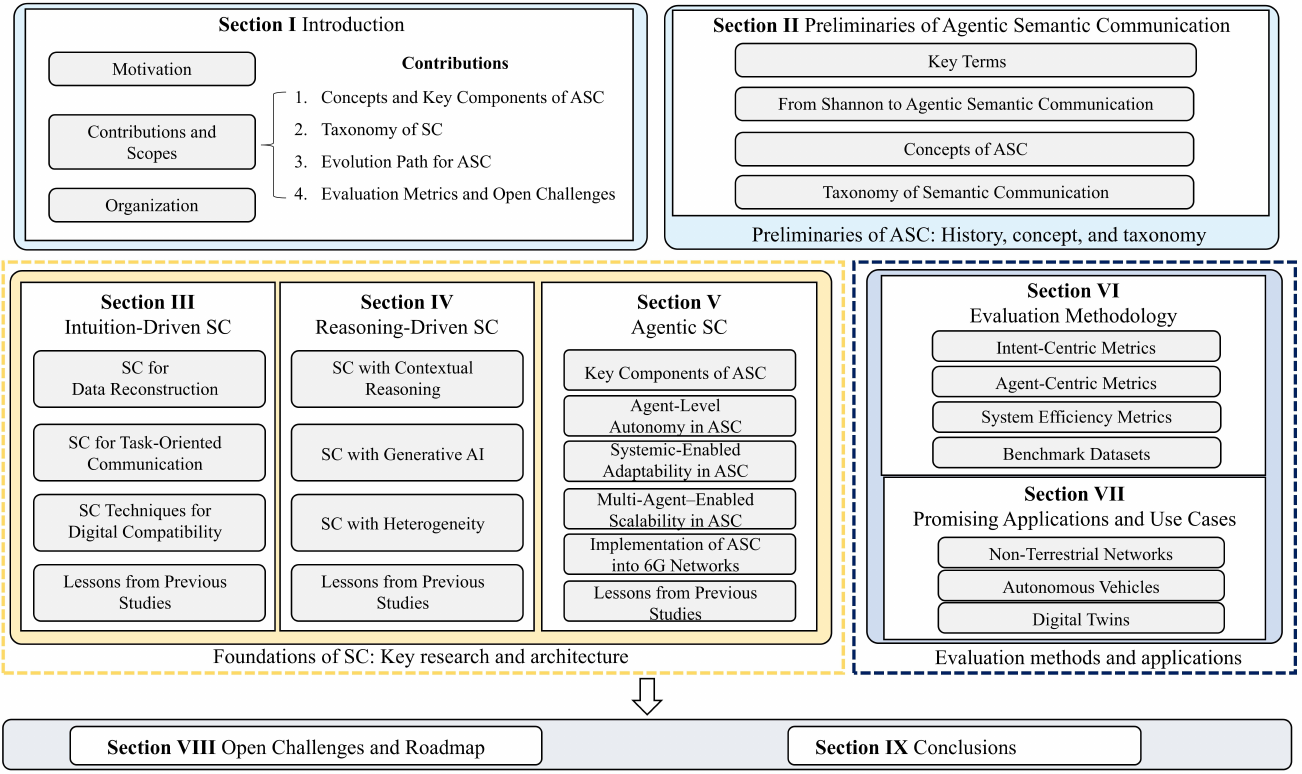
\includegraphics[width=\linewidth]{fig/fig1.png}
\caption{서베이의 구성.}
\label{fig:1}
\end{figure}

이 서베이는 ASC의 지형을 규정하는 세 가지 근본 연구 질문(RQ, research question)을 다룬다.
\begin{enumerate}[label=\arabic*)]
\item \textbf{RQ1 -- ASC의 구조 설계:} 어떤 설계 원칙이 있어야 ASC 시스템에서 에이전트가 맥락을 효율적으로 공유하고, 의미를 협상하고, 자율적으로 결정을 내릴 수 있는가?
\item \textbf{RQ2 -- ASC에서의 학습과 적응:} ASC에서 의미를 파악하고 추론을 수행하는 데, 특히 자율성에 기반할 때, 어떤 학습 전략이 효과적인가?
\item \textbf{RQ3 -- 의도 평가:} ASC 시스템은 의미 정렬과 의도 보존을 어떻게 측정할 수 있는가?
\end{enumerate}

이 세 연구 질문을 다룸으로써 얻은 이 서베이의 기여는 다음과 같이 요약할 수 있다.
\begin{itemize}
\item \emph{ASC의 개념과 핵심 구성 요소} (\textbf{RQ1}): 필수 구성 요소를 통합해 ASC 프레임워크를 개념화한다. 통신 환경에 내재한 제약 안에서 새로운 지능 요소(예: LLM, 세계 모델, KB)가 더해질 때 이 기술들을 어떻게 다시 생각해야 하는지 설명한다.
\item \emph{SC의 분류 체계} (\textbf{RQ1, RQ2}): SC 방식을 추론 능력과 적응성 수준에 따라 분류한다. SC 시스템을 구조나 AI 기법으로 분류한 기존 서베이와 달리, 제안하는 분류 체계는 세 가지 통신 설계 축, 곧 지식의 위치, 의미를 추론하는 과정, 적응적 추론(inference)-추론(reasoning) 제어의 유무를 따라 구성된다.
\item \emph{ASC로의 진화 경로} (\textbf{RQ2}): LLM 기반 추론, 세계 모델, 다중 에이전트 조정이 자원과 채널 제약 아래에서 \emph{무엇을}, \emph{언제}, \emph{어떻게} 통신할지라는 질문에 답하는 통신 인지형(communication-aware) 구성 요소로 어떻게 구현되는지 살펴보고, 이를 통해 ASC의 연구 방향을 제시한다.
\item \emph{평가 지표와 미해결 과제} (\textbf{RQ2, RQ3}): 의도 정렬과 에이전트 상호작용을 중심으로 한 평가 지표를 제시하고 벤치마크를 논의한다. 더 나아가 현재 ASC 연구에서 충분히 다루어지지 않은 미해결 과제를 밝힌다.
\end{itemize}

이 연구는 맥락 지식이 없는 초기 SC 모델부터 추론 능력을 갖춘 ASC까지를 포괄하는 서베이를 제공한다. 핵심 주장은 ASC의 새로움이 개별 AI 모듈 자체가 아니라, 통신을 인식하는 방식으로 이 모듈들을 구현하고 시스템 수준에서 공동 설계하는 데 있다는 것이다. 구체적으로 LLM 기반 추론, 계획, 적응적 상호작용, 협력 추론(cooperative inference)을 포함한 ASC의 핵심 기술을 기술한다. 과업 성공 확률, 지연-보상 절충(trade-off) 같은 에이전트형 평가 지표를 검토하고, 벤치마크 데이터셋을 논의한다. 이 서베이는 비지상 네트워크, 자율주행차, 디지털 트윈(digital twin)을 포함한 유망한 ASC 응용을 살펴보고, 미해결 과제를 개괄하며, 향후 연구를 위한 로드맵을 제시한다.

\subsection{구성}
서베이의 구조는 그림~\ref{fig:1}에 나타냈다. 이 서베이의 나머지 부분은 다음과 같이 구성된다. II절에서는 SC에서 ASC로의 진화를 검토하고 ASC의 핵심 개념과 분류 체계를 소개한다. III절에서는 시스템 1 유형으로 특징지어지는 SC 방법을 포괄적으로 조사한다. IV절에서는 시스템 2 유형을 구현한 SC 연구를 기술한다. V절에서는 ASC의 대표적 방법을 소개한다. ASC의 평가 지표와 벤치마크 데이터셋은 VI절에서 기술한다. ASC의 대표적 응용 시나리오와 활용 사례는 VII절에서 살펴본다. 미해결 과제와 향후 연구 방향은 VIII절에서 제안한다. 맺음말은 IX절에 있다.

\section{에이전트형 SC의 기초}

\setcounter{figure}{1}
\begin{figure}[htbp]
\centering
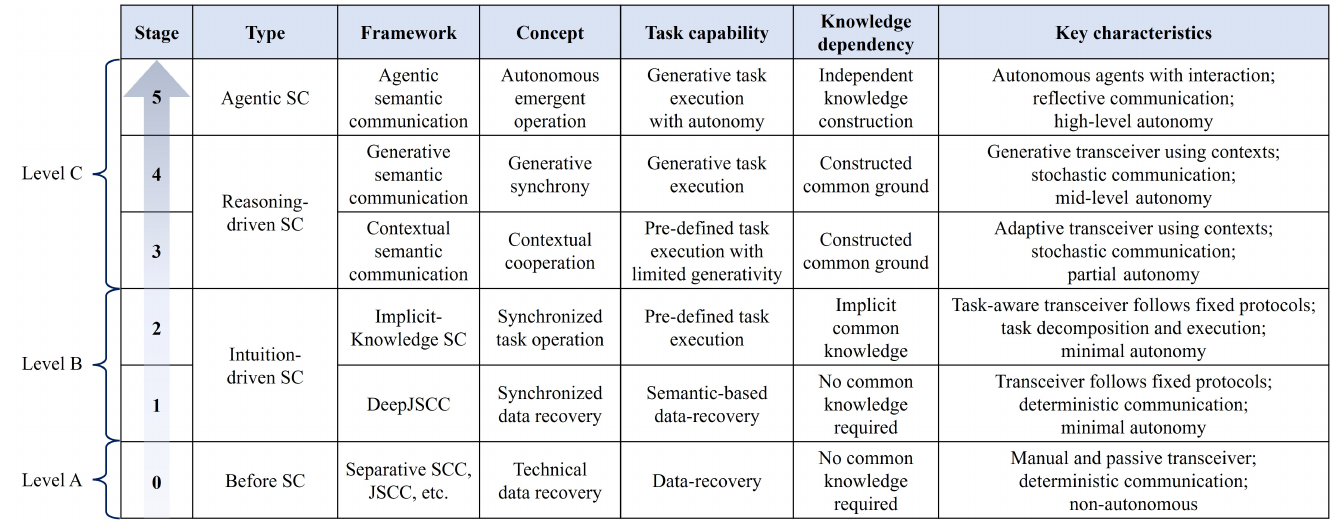
\includegraphics[width=\linewidth]{fig/fig2.png}
\caption{에이전트형 SC로 가는 진화 경로.}
\label{fig:2}
\end{figure}

\setcounter{table}{1}
\begin{table}[htbp]
\centering
\caption{이 글에서 쓰는 핵심 용어}
\label{tab:2}
\small
\renewcommand{\arraystretch}{1.2}
\begin{tabularx}{\linewidth}{|>{\centering\arraybackslash}p{0.2\linewidth}|Y|}
\hline
\textbf{용어} & \centering\arraybackslash\textbf{정의} \\
\hline
\textbf{의도(Intent)} & 송신자가 이루고자 하는 결과로, 전송된 메시지의 기호적 내용 너머에 있다. \\
\hline
\textbf{의미 정렬(Semantic Alignment)} & 상호작용과 추론을 거쳐 메시지의 의미에 대한 공통 이해(공유 맥락)에 이르는 과정과 그 상태. \\
\hline
\textbf{의도 보존(Intent Preservation)} & 의미 정렬이 성공적으로 이루어졌음을 결과 수준에서 보장하는 것. \\
\hline
\textbf{추론(Inference)} & 학습된 모델이 입력이 주어졌을 때 출력을 내는 과정. \\
\hline
\textbf{생성(Generation)} & 학습된 확률 분포에서 표본을 추출해 모델이 새로운 내용을 만들어 내는 추론의 한 형태. \\
\hline
\textbf{추론(Reasoning)} & 모델이 결론에 이르기 전에 중간 논리 단계를 명시적으로 거치는 구조화된 추론 과정으로, 이 글에서는 시스템 2 유형의 처리에 해당한다. \\
\hline
\textbf{사고(Thinking)} & 최종 출력 전까지 중간 단계가 드러나지 않는, 내재화된 형태의 추론. \\
\hline
\textbf{ASC 에이전트(ASC Agent)} & 지각--기억--정책--통신--갱신 루프를 지닌 개체. \\
\hline
\textbf{자율성(Autonomy)} & 외부 지시 없이 자신의 목표를 추구하는 에이전트의 능력. \\
\hline
\end{tabularx}
\end{table}

\subsection{핵심 용어}
이 글 전반에서 쓰는 핵심 용어(예: 의도, 의미 정렬, 의도 보존 등)를 표~\ref{tab:2}에 정리했다.

이 글에서는 \emph{과업 지향}(task-oriented), \emph{의도 기반}(intent-based), \emph{의미 지향(의미적)}(meaning-oriented (semantic)) 통신이라는 용어를 두루 쓴다. 이 용어들은 서로 다른 설계 목표, 최적화 대상, 성공 기준을 가리킨다. 표~\ref{tab:3}은 이들을 구분하고, 이 서베이가 각 단계에서 어떤 개념을 채택하는지 명시한다. III절과 IV절은 의미 지향 설계와 과업 지향 설계를 다루고, V절은 의도 지향(효과 수준) 설계를 다룬다.

\setcounter{table}{2}
\begin{table}[htbp]
\centering
\caption{의미 지향, 과업 지향, 의도 기반 통신의 구분}
\label{tab:3}
\small
\renewcommand{\arraystretch}{1.2}
\begin{tabularx}{\linewidth}{|>{\centering\arraybackslash}p{0.17\linewidth}|>{\centering\arraybackslash}X|>{\centering\arraybackslash}X|>{\centering\arraybackslash}X|}
\hline
\textbf{측면} & \textbf{의미적} & \textbf{과업 지향} & \textbf{의도 기반} \\
\hline
Weaver 수준 & 수준 B & 수준 B--C & 수준 C \\
\hline
전송하는 것 & 원천의 의미를 복구하기 위한 표현 & 알려진 하위(downstream) 과업을 위한 표현 & 의도나 제약을 위한 표현 \\
\hline
최적화 대상 & 원천과 복원 사이의 의미 충실도 & 과업 손실 & 과업 성공과 의도 보존 \\
\hline
설계 단계에서 과업을 아는가? & 반드시 그렇지는 않음 & 예 & 아니요. 추론하거나 협상함 \\
\hline
\end{tabularx}
\end{table}

\subsection{Shannon에서 에이전트형 SC까지}
Shannon--Weaver 모델의 수준 A에서 정보는 메시지의 통계적 불확실성으로 구문적으로(syntactically) 정의되며, 그 발생 확률로 측정된다. 따라서 메시지의 의미적 불확실성은 무시될 수 있다. 예를 들어 수준 A에서는 의미 있는 메시지와 의미 없는 메시지가 같은 양의 정보를 담을 수 있다. 이 경우 의미 오류는 수준 A에서 표현되지 않으므로 바로잡기 어렵다. Shannon은 이 한계를 핵심 과제 가운데 하나로 꼽았으며 [4], Weaver는 통신을 기술적 정확성(수준 A), 의미 해석(수준 B), 행동 효과(수준 C)의 세 수준으로 구성했다 [1].

Shannon--Weaver 모델과 달리, 우리는 이 세 수준을 ASC를 향한 구현 지향 단계로 재구성한다. 그림~\ref{fig:2}는 통신 시스템의 진화를 보여 준다. SC 이전(Before SC)은 수준 A에 해당하는 단계 0이다. 여기서 결정론적 통신(deterministic communication)이란 고정된 프로토콜 아래에서 전송 동작이 미리 정해진 통신을 뜻한다. 단계 1과 2는 기호 복구보다 과업 지향 의미를 우선하며 수준 B를 구현한다. 단계 3, 4, 5는 수준 C에 해당하며, 지식을 통합하고 통신 의도를 정렬한다. SC 이전을 제외하면 통신 유형은 직관 기반 SC, 추론 기반 SC, ASC로 분류된다. SC와 관련된 유형은 분류 체계 소절에서 자세히 다룬다.

6G 비전이 등장하면서 초당 테라비트(Tbps, terabit-per-second) 링크의 필요성과 기계학습(ML, machine learning)의 활용으로 의미 효율이 주목받게 되었다 [16]. 입력 데이터를 단순히 압축한 전송 비트 대신, 수신기가 과업을 수행하는 데 필요한 관련 정보를 전송하는 것이 중요해졌다. 이 요구가 수준 B와 수준 C의 의제를 되살렸고, 이것이 초기 SC의 시작이 되었다 [5].

초기 SC 프레임워크는 송신자와 수신자를 하나의 결합된 심층 오토인코더로 보았다. 초기 SC 모델인 딥러닝 기반 결합 원천-채널 부호화(DeepJSCC, deep learning-based joint source and channel coding) [5]는 단계 1로의 전환을 대표한다. DeepJSCC 모델은 원시 데이터 입력을 저차원 의미 임베딩으로 부호화하고 수신기 쪽에서 이를 복호한다. 그러나 이 방식은 의미 전달보다는 효율적인 데이터 복구에 주로 초점을 맞춘다. 더욱이 공통 지식이 필요 없으므로 지식을 전달하는 능력이 제한된다.

단계 2로서, 이미지 [5]--[7], 음성 [8], 텍스트 [9]의 의미 충실도를 높이는 유망한 해법으로 암묵 지식 SC(implicit-knowledge SC) 방법들이 제안되었다. 수많은 연구가 SC의 초기 개념을 이미지, 음성, 다중 모달 데이터에 적용했다 [6]--[9], [24], [25]. 그러나 초기 SC 연구 대부분은 암묵적 KB와 고정 프로토콜을 갖춘 쌍 설정을 가정했다. 이 가정으로는 에이전트들이 서로 다른 맥락 지식을 지닐 때 생기는 맥락 정렬 문제를 다룰 수 없다. 고수준 통신에서는 송신자와 수신자 사이에 동적인 의미 정렬과 의도 이해가 흔히 요구된다. 수신자가 기호를 복원하더라도 송신자의 의도를 오해할 수 있다.

맥락 불일치를 완화하기 위해 KB가 그래프 형태로 의미 부호기와 복호기에 통합되었다 [11], [12]. 이것이 단계 3에 해당한다. 입력을 그래프의 삼중항(triple)에 대응시킴으로써, 시스템은 과업과 관련된 추론에 필요한 노드에 데이터를 압축한다. KB를 구현하면 의미적 모호성을 줄일 수 있다. 그러나 남은 몇 가지 문제는 충분히 해결하지 못한다. 첫째, KB는 여전히 낡았거나 사용자 사이에 비대칭일 수 있다. 둘째, 상호작용이 일회적(episodic)이어서 오해가 생겼을 때 의미를 협상할 장치가 없다. 마지막으로, 기존 SC 프레임워크는 흔히 쌍으로 된 시스템 1 유형 SC를 가정하므로 [14], 과업이 바뀔 때 적응성이 제한된다.

이러한 간극을 메우려면, 의도한 의미가 정확히 해석되도록 시스템 2의 추론 능력이 필요하다. 맥락 정렬의 부족을 해결하기 위해 추론 능력을 갖춘 SC 방법 [26]이 제안되었다. 대표적 예가 단계 4로 나타낸 생성형 SC(GSC, generative SC)이다. 시스템 1 기반 SC 프레임워크와 달리, GSC에서는 수신기의 생성 과정으로 의미적 모호성을 해소할 수 있다. 수신기에서 원래 의미를 복원하는 대신, 송신자의 맥락을 이용해 의도를 풀어내어(decapsulate) 의미 정렬을 돕는다. 추론 능력이 있음에도, GSC는 생성 모델 고유의 계산 복잡도 때문에 시스템에 부담을 줄 수 있다. 엣지 네트워크처럼 자원과 추론 시간이 제한된 특정 통신 시스템에서는 GSC를 채택하는 것이 실시간 추론에 불리할 수 있다. 따라서 모호한 과업을 효율적으로 수행하려면 시스템 1과 시스템 2의 기능을 모두 수행할 수 있는 향상된 시스템이 필요하다 [13], [14]. 단계(Step) 5에서 기술하는 ASC는 이러한 시스템의 계산 부담을 해결하는 효과적인 해법이 될 수 있다. ASC는 효율적인 추론을 기본으로 쓰고 불확실성이 높거나 분포 밖(OOD, out-of-distribution)인 조건에서만 추론(reasoning)을 호출함으로써, GSC의 지연 비용을 항상 치르지 않고도 강건성을 높일 수 있다. 또한 신경-기호(NeSy, neuro-symbolic) AI는 신경망 기반 특징 추출과 규칙 기반 기호 추론을 결합한다 [27]. 송신자와 수신자가 온톨로지와 추론 규칙 같은 기호 규약을 이미 공유하고 있으면, 고차원 특징 벡터 대신 간결한 기호를 전송할 수 있다. 그러면 메시지당 전송 비용이 줄어드는 대신, 이러한 규약을 미리 배포하고 동기화하는 비용이 든다. ASC 안에서는 에이전트 사이에 KB가 갱신되므로 의미적 모호성을 완화할 수 있다. 전환 기능이 더해지면, GSC의 약점으로 지적된 실시간 추론 면에서도 이점이 생길 것이다.

\subsection{ASC의 개념}
\paragraph{1) 시스템 1과 시스템 2:} 시스템 1과 시스템 2는 의사결정에 대한 상호 보완적인 두 접근을 설명하는 두 개념이다. 시스템 1은 빠르고 직관적이며, 휴리스틱 처리에 의존해 즉각적인 반응을 가능하게 한다. 반면 시스템 2는 더 느리고 신중하게 동작한다. 제안하는 ASC 프레임워크에서는 이 두 개념이 통합된다. 이 이중 시간 척도 동작은 6G 무선 접속 네트워크의 제어 루프와 닮았다. 시스템 1 유형의 추론은 준실시간(near-real-time) 무선 접속 네트워크(RAN, radio access network) 지능형 제어기(RIC, RAN intelligent controller) 루프에, 시스템 2 유형의 추론(reasoning)은 비동기로 동작하는 비실시간(non-real-time) RIC 루프에 대응한다. 표준화된 준실시간(near-RT) RIC 루프는 10~ms--1~s에 걸치지만, 최근의 한 구현은 xApp을 기저대역 장치(baseband unit)와 같은 곳에 배치해 10~ms 미만의 추론을 보고했다 [28]. 이 대응 관계는 V-E절에서 다시 다룬다. 시스템 1, 시스템 2, ASC의 특성은 표~\ref{tab:4}에 종합해 정리했다.

\setcounter{table}{3}
\begin{table}[htbp]
\centering
\caption{시스템 1, 시스템 2, ASC의 특징}
\label{tab:4}
\small
\renewcommand{\arraystretch}{1.2}
\begin{tabularx}{\linewidth}{|>{\centering\arraybackslash}p{0.14\linewidth}|>{\centering\arraybackslash}X|>{\centering\arraybackslash}X|>{\centering\arraybackslash}X|}
\hline
\textbf{특징} & \textbf{시스템 1} & \textbf{시스템 2} & \textbf{ASC (시스템 1과 시스템 2)} \\
\hline
\textbf{인지 과정} & 빠름, 휴리스틱, 직관적 & 더 느림, 논리적, 부담이 큼 & 적응적, 성찰적 \\
\hline
\textbf{핵심 기능} & 패턴 인식, 확률적 추론 & 인과적 추론, 논리적 추론 & 신경-기호 AI, 인지적 성찰 \\
\hline
\textbf{SC에서의 역할} & 효율적인 데이터 복원 & 의미 정렬, 모호성 해소 & 자율적 계획, 맥락 적응 \\
\hline
\end{tabularx}
\end{table}

시스템 1과 시스템 2의 도입은 ML 분야에서 오랫동안 논의되어 온 주제이다. Bengio [29]는 시스템 1 유형 ML에서 시스템 2 유형 ML로 나아가는 연구 방향을 제시했고, Bo Zhang 등 [30]은 시스템 1 유형 ML을 시스템 2 유형 ML에 통합할 것을 주장했다. 이러한 선행 주장에 영향을 받아, 연구자들은 범용 인공지능(AGI, artificial general intelligence)에 이르려면 추론과 패턴 인식을 통합해야 한다는 데 의견을 같이한다. 그 결과 최근 연구는 시스템 1 유형과 시스템 2 유형 ML을 상호 보완적으로 보고 그 통합에 초점을 맞춘다.

이전의 딥러닝 기반 모델 대부분은 방대한 학습 데이터를 활용해 패턴 인식에서 뛰어난 성능을 보였다 [31]. 이러한 모델은 시스템 1 유형 ML 모델로 볼 수 있다. 이 모델들은 인과적 추론 없이 데이터의 통계적 패턴을 내재화하고 확률적 출력을 추론한다. 대표적인 시스템 1 유형 ML 모델인 GPT-4o [32]는 적절한 토큰을 예측하여 적절한 문장을 생성한다. 그러나 경험적 증거에 따르면 논리적 사고가 필요한 과업에서는 환각(hallucination)이 성능을 떨어뜨릴 수 있다 [33]. 시스템 1 유형 ML의 한계를 보완하기 위해 인지적 측면을 반영한 추론 기반 방법론들이 제안되었다 [34]--[36].

최근에는 시스템 1 유형과 시스템 2 유형 ML의 장점을 결합하는 연구가 제안되었다 [27], [37]. 의사결정에 대한 이중 시스템 접근에 기반해 Talker-Reasoner 구조가 제안되었다 [37]. 지연이 짧은 Talker(시스템 1)가 간단한 질의를 처리하고, 불확실성이 높은 사례를 처리할 때는 Reasoner(시스템 2)를 호출한다. NeSy AI를 이용한 또 다른 통합 접근도 제안되었다 [27]. 이 프레임워크에서 에이전트는 인지적 성찰(cognitive reflection)이라는 개념으로 효율과 효과 사이의 균형을 맞출 수 있다. 인지적 성찰이란 자신의 처음 직관적 반응을 점검하고 추론을 거쳐 의도적으로 수정하는 메타인지 과정을 말한다 [27]. 에이전트는 직관적(시스템 1) 답이 기호적(시스템 2) 지식과 모순될 때마다 인지적 성찰을 이용해 그 답을 자동으로 바로잡는다.

\setcounter{figure}{2}
\begin{figure}[htbp]
\centering
\begin{minipage}{0.8\linewidth}\centering
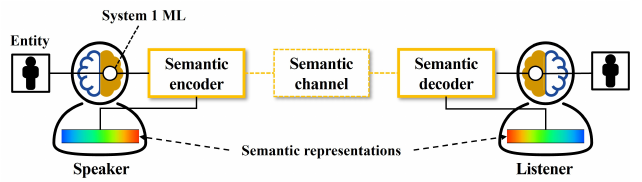
\includegraphics[width=\linewidth]{fig/fig3a.png}\\[0.2em]
{\small (a) 시스템 1 유형 ML을 쓰는 SC}
\end{minipage}\par\vspace{0.8em}
\begin{minipage}{0.8\linewidth}\centering
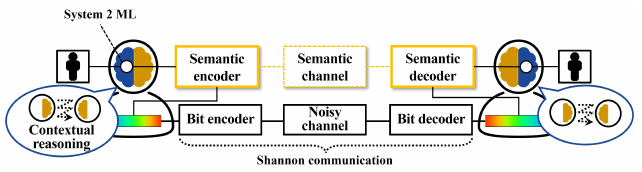
\includegraphics[width=\linewidth]{fig/fig3b.png}\\[0.2em]
{\small (b) 시스템 2 유형 ML을 쓰는 SC}
\end{minipage}\par\vspace{0.8em}
\begin{minipage}{0.8\linewidth}\centering
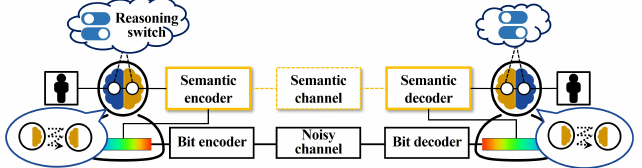
\includegraphics[width=\linewidth]{fig/fig3c.png}\\[0.2em]
{\small (c) 시스템 1 유형과 2 유형 ML을 통합한 SC}
\end{minipage}
\caption{(a) 시스템 1 유형 ML을 쓰는 SC, (b) 시스템 2 유형 ML을 쓰는 SC, (c) 시스템 1 유형과 2 유형 ML을 통합한 SC의 개념도. [13]의 그림을 수정한 것이다.}
\label{fig:3}
\end{figure}

시스템 2 유형 ML에 대한 관심은 커졌지만, SC에 대한 적용은 제한적이었다. SC 프레임워크는 시스템 2 유형 ML 대신, 빠른 추론에 최적화된 시스템 1 유형 ML에 주로 의존해 왔다. Seo [13], Bennis [14], Walid [38]의 연구처럼 최근의 이론적 시도들이 SC의 추론 능력을 논의했지만, 이들은 개념적 측면에 초점을 맞추었다. SC 시스템에 추론 능력을 부여하기 위해 생성형 AI(GAI, generative AI)를 통합하는 접근 [39]이 제안되었다. 그러나 GAI 추론을 계속 호출하면 상당한 지연이 생길 수 있다. 딥러닝 응용과 달리, 대부분의 통신 시스템에서는 추론 지연이 심각한 문제가 될 수 있다. 이 문제를 해결하려면 그림~\ref{fig:3}(c)처럼 SC 프레임워크에 이중 경로 추론 구조를 도입해야 한다.

\paragraph{2) 창발 언어:} 창발 언어(EmLang)는 미리 정의된 프로그래밍 없이 에이전트들의 상호작용에서 자연스럽게 생겨나는 통신 메커니즘을 말한다 [40]. 사람이 설계하는 하향식 패러다임과 달리, EmLang은 통신 프로토콜이 상호작용으로부터 적응적으로 진화하는 상향식 패러다임을 따른다 [41]. EmLang에서는 에이전트들이 주어진 환경 안에서 협력 과업을 풀며, 그 결과로 기호 구조가 발달한다.

ASC는 EmLang의 개념을 받아들여, 에이전트가 통신 행동을 계속 조정하는 상호작용 학습 환경을 가정한다. 이 맥락에서 ASC는 다중 에이전트 강화학습(MARL, multi-agent reinforcement learning)이나 부분 관측 마르코프 결정 과정(POMDP, partially observable Markov decision process) 설정으로 볼 수 있다. 이러한 환경에서 에이전트들은 상호작용하며 메시지를 반복적으로 교환한다. 처음에는 에이전트 사이에 오가는 토큰이 무작위 기호로 이루어진다. 이후 에이전트들은 전송된 기호, 환경 상태, 자기 행동의 결과 사이의 연관을 거듭 찾아낸다. 반복된 상호작용을 거쳐 에이전트들은 의미 있는 표현을 형성하고, 이 표현은 협력 효용을 최적화하는 기호로 수렴한다.

\paragraph{3) 에이전트형 AI, 체화 AI, ASC:} AI 분야에서는 단일 과업 모델을 넘어서는 에이전트를 만드는 데 초점을 둔 새로운 패러다임이 등장했다. 이 에이전트들은 목표를 세우고 과업을 실행할 수 있다. 에이전트형 AI(Agentic AI)라 불리는 이 새로운 패러다임은 불확실하고 동적인 환경에서 목표를 이루기 위한 자율적 지각, 계획, 행동, 학습을 특징으로 한다.

에이전트형 AI와 비슷하지만 구별되는 개념으로 체화 AI(Embodied AI)가 있다. 둘 다 환경과의 상호작용으로 정책을 학습하지만, 체화 AI는 지각과 행동을 완전히 통합된 과정으로 본다. 예를 들어 탁자 위의 사과를 집어 드는 목표를 지닌 로봇이 있다고 하자. 체화 AI에서는 시각 입력과 모터 명령이 되먹임 루프 안에서 동시에 갱신된다. 이 방식은 대개 연속적인 상태 공간과 행동 공간을 지니며, 에이전트는 물리 환경과 상호작용하며 최적 정책을 학습한다. 또한 최근의 체화 AI는 세계 모델을 환경에 대한 사전 지식으로 활용해 미래의 환경 상태를 예측하고 의사결정을 이끈다 [42].

\setcounter{table}{4}
\begin{table}[htbp]
\centering
\caption{체화 AI, 에이전트형 AI, ASC의 특징}
\label{tab:5}
\small
\renewcommand{\arraystretch}{1.2}
\begin{tabularx}{\linewidth}{|>{\centering\arraybackslash}p{0.14\linewidth}|>{\centering\arraybackslash}X|>{\centering\arraybackslash}X|>{\centering\arraybackslash}X|}
\hline
\textbf{특징} & \textbf{에이전트형 AI} & \textbf{체화 AI} & \textbf{에이전트형 SC} \\
\hline
\textbf{범위} & 제어 시스템, 문제 해결 & 로봇공학, 감각운동 과업 & 통신 중심 과업 \\
\hline
\textbf{핵심 기능} & 지각, 계획, 행동, 학습 & 지각과 행동의 결합 & 의미 추출, 계획, 상호작용, 적응 \\
\hline
\textbf{목표} & 목표를 위한 적응적 의사결정 & 물리적 상호작용을 통한 최적 정책 & 의미 충실도, 통신 효율 \\
\hline
\textbf{지식 활용} & 장기 기억, 광범위한 추론 & 물리적 사전 지식 & 중간 수준 기억, 적응적 추론 \\
\hline
\end{tabularx}
\end{table}

ASC는 에이전트형 AI의 일부 원리를 물려받은, 통신 중심 과업의 전문가로 볼 수 있다. 두 시스템은 핵심 속성을 공유하지만 관점은 조금 다르다. 예를 들어 에이전트형 AI는 자율주행, 로봇 제어, 네트워크 관리를 포함한 넓은 영역에서 지각, 계획, 행동, 학습을 다루는 데 쓰여 왔다 [2]. 반면 ASC 시스템은 의미 프로토콜 안에서의 계획, 상호작용, 적응적 동작으로 초점을 좁히며, 지각은 과업 지향 의미 추출로 한정한다. 또한 에이전트형 AI는 장기 기억과 광범위한 추론으로 효과적인 의사결정을 목표로 하는 반면, ASC는 효율적인 통신을 위해 중간 수준 기억(moderate memory)과 적응적 추론을 쓴다. 여기서 장기 기억은 세션을 넘어 유지될 수 있다는 점에서, 에이전트 사이에 공유되는 구조화된 지식을 담은 KB와 구별된다. 반면 중간 수준 기억은 최근의 의미 표현을 수 초에서 수 분 동안 유지하는, 세션 범위의 의미 기억이다. 세 시스템 모두 목표 지향적 행동을 보이지만, 동작 환경의 성격, 행동의 양식, 추론의 범위에서 다르다. 에이전트형 AI, 체화 AI, ASC의 차이는 표~\ref{tab:5}에 요약했다.

\setcounter{figure}{3}
\begin{figure}[htbp]
\centering
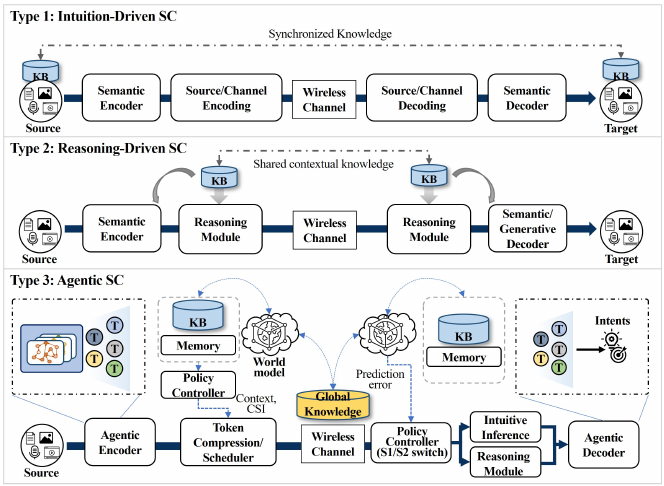
\includegraphics[width=0.85\linewidth]{fig/fig4.png}
\caption{제안하는 의미 통신 시스템 분류 체계의 대표 구조.}
\label{fig:4}
\end{figure}

\subsection{의미 통신의 분류 체계}
앞에서 논의한 시스템 1/2, 명시적 지식, 에이전트형 제어를 바탕으로, 이 소절에서는 SC 시스템의 분류 체계를 소개한다. 기존 SC 분류 체계는 주로 응용 영역 관점(예: 과업 지향 대 데이터 복원), 입력 모달리티, 외부 지식 활용과 자원 제약에 따라 분류한다 [16], [20], [22]. 이러한 관점으로는 시스템이 변화하는 환경에서 어떻게 추론하고 적응하는지를 충분히 설명하지 못한다. 암묵적 추론에서 명시적 추론과 적응적 오케스트레이션으로의 전환에 착안하고 이중 과정 인지에서 영감을 받아, 우리는 SC 시스템을 세 가지 주요 축으로 정리한다. (i) 의미 지식이 어디에 있는가. 학습된 매개변수 안에 암묵적으로 있는가, 외부 지식 구조에 명시적으로 있는가. (ii) 의미를 어떻게 추론하는가. 순방향(feed-forward) 사상으로 하는가, 명시적인 맥락·모델 기반 추론이나 생성적 완성으로 하는가. (iii) 적응적 제어 모듈이 추론(inference)과 추론(reasoning) 사이를 전환하는가. 이 기준에 따라 기존 SC 방법은 직관 기반 SC, 추론 기반 SC, ASC의 세 유형으로 분류할 수 있다.
\begin{itemize}
\item \textbf{직관 기반 SC}: 직관 기반 SC 시스템은 명시적 추론 모듈이나 적응적 추론(inference)-추론(reasoning) 제어 없이, 의미 부호기와 복호기를 함께 학습시켜 의미 표현을 암묵적으로 부호화한다. 이 설계는 일상적인 과업에서는 효과적으로 동작할 수 있지만, 학습된 사상이 분포 변화에 민감하여 OOD에 대한 강건성이 제한된다 [10], [43].
\item \textbf{추론 기반 SC}: 추론 기반 SC 시스템은 KB, 생성 모델, 추론 모듈 같은 외부 또는 공유 맥락 지식을 명시적으로 포함하여 맥락을 고려한 의미 표현을 구성한다. 맥락 지식을 명시적으로 쓰면 일반적으로 OOD 조건에서 강건성이 높아진다 [11], [44]. 그러나 과업의 복잡도와 관계없이 추론 과정을 늘 수행하므로, 직관 기반 SC 시스템보다 계산 오버헤드가 크다 [39]. 예를 들어 확산 모델 또는 LLM 기반 추론은 출력 하나를 얻는 데 순방향 패스 한 번이 아니라 수십에서 수백 번의 순차적 네트워크 평가가 필요하다.
\item \textbf{에이전트형 SC}: ASC는 기억, 세계 모델, 전역 지식, 토큰 스케줄링·압축, 정책 제어기 같은 구성 요소를 추가로 도입해 추론 기반 SC를 확장한다. 추론 기반 SC와 달리 ASC는 예상 불확실성에 따라 시스템 1 추론(inference)과 시스템 2 추론(reasoning) 사이를 적응적으로 전환한다. 이러한 에이전트형 제어는 SC 시스템의 자율성을 높이고, 복잡한 과업을 처리할 때 강건성과 계산 효율 사이의 균형을 유지한다 [13], [37]. 자세한 내용은 V절에서 다룬다.
\end{itemize}

\setcounter{table}{5}
\begin{table}[htbp]
\centering
\caption{SC 시스템의 주요 분류 체계와 설계 특징}
\label{tab:6}
\small
\renewcommand{\arraystretch}{1.2}
\begin{tabularx}{\linewidth}{|>{\centering\arraybackslash}p{0.16\linewidth}|>{\centering\arraybackslash}X|>{\centering\arraybackslash}X|>{\centering\arraybackslash}X|}
\hline
\textbf{특징} & \textbf{직관 기반 SC} & \textbf{추론 기반 SC} & \textbf{에이전트형 SC} \\
\hline
\textbf{지식 위치} & 주로 암묵적 & 외부 지식 & 동적으로 갱신되는 지식 \\
\hline
\textbf{추론 방식} & 순방향 사상 & 명시적 맥락·모델 기반 추론 & 혼합형 (시스템 1 + 시스템 2) \\
\hline
\textbf{OOD 강건성} & 낮음 & 중간~높음 & 높음 \\
\hline
\textbf{지연--성능 절충} & 짧은 지연, 제한된 적응성 & 더 긴 지연, 향상된 강건성 & 적응적 지연--성능 절충 \\
\hline
\end{tabularx}
\end{table}

분류 체계의 구조적 차이는 표~\ref{tab:6}과 그림~\ref{fig:4}에 나타냈다. OOD 강건성은 각 유형의 구조적 능력에 근거해 정성적으로 평가했다. 직관 기반 SC는 종단간(end-to-end) 학습과 분포 변화에 대한 민감성 때문에 강건성이 낮다. 추론 기반 SC는 KB와 생성 모델을 활용해 부분적인 일반화를 제공하므로 강건성이 중간에서 높은 수준이다. 분포 변화가 공유 KB나 생성 사전(prior)으로 포괄되면 과업 성능을 유지하지만, 그렇지 않으면 성능이 떨어진다. 세계 모델, 자기 교정, 이중 시스템 처리를 갖춘 ASC는 강건성이 높다. 표~\ref{tab:6}의 지연에 관해 말하면, 짧은 지연은 단일 추론 패스에 해당하고, 긴 지연은 반복적 추론(reasoning)을 요구한다. ASC는 평소에는 시스템 1로 동작하고, 불확실성이 높을 때만 시스템 2를 호출한다.

그림~\ref{fig:4}에서 보듯이, 직관 기반 SC 시스템은 한 쌍의 의미 부호기와 복호기로 이루어지며, 이는 오토인코더 구조로 구현되어 왔다. 추론 기반 SC 시스템은 명시적 KB와 추론 모듈을 포함한다. 시스템 설계에 따라 수신기는 의미 복호기나 생성 복호기를 써서 수신된 표현으로부터 목표 내용을 추론할 수 있다. ASC는 기억, KB, 세계 모델, 정책 제어기를 통합해 의미 송수신을 적응적으로 처리한다. 정책 제어기는 예측된 불확실성, 맥락, 채널 상태 정보(CSI, channel state information), 예측 오차에 따라 시스템 1 추론(inference)과 시스템 2 추론(reasoning) 사이를 동적으로 전환하여 효율을 높인다. 그림~\ref{fig:4}의 채널을 무선 링크로 그린 것은 조사한 SC 시스템 대부분이 무선 시나리오를 대상으로 하기 때문이며, 분류 체계 자체는 채널에 무관하다.

% part_B: 원문 8쪽 III절 ~ 13쪽 IV-D절 끝 (그림 5, 6 / 표 VII, VIII)

\section{직관 기반 의미 통신}

\subsection{데이터 복원을 위한 의미 통신}

직관 기반 의미 통신(SC)은 의미 부호기와 의미 복호기로 이루어진 종단 간 구조 위에 세워졌으며, 처음에는 단일 모달리티 데이터를 전송하고 복원하기 위해 개발되었다.
여러 모달리티 가운데 이미지, 텍스트, 음성이 흔히 쓰였는데, 주된 이유는 이들이 높은 데이터 전송률을 요구하기 때문이다.
특히 결합 원천-채널 부호화(JSCC, joint source-channel coding)에 기반한 종단 간 딥러닝 방식이 널리 쓰인다.

\paragraph{1) 이미지 복원}
최초의 방식인 DeepJSCC는 합성곱 신경망(CNN, convolutional neural network) 기반 오토인코더 구조로 무선 채널에서 이미지를 효율적으로 전송할 수 있음을 보였다 [5].
원천 부호화와 채널 부호화를 따로 수행하는 기존 전송 시스템과 달리, 이 방식은 두 부호화를 결합해 최적화함으로써 복원에 필요한 특징을 보존한다.
예를 들어 낮은 SNR에서 복원 이미지는 기존 분리 설계에서 나타나는 급격한 절벽 효과(cliff effect)를 보이지 않는다. 그 대신 전체 객체 구조는 유지한 채 미세한 질감을 점차 잃는다.
이를 바탕으로 이미지 복원을 위한 다양한 SC 방식이 제안되었다 [6], [7].
그 가운데 되먹임을 쓰는 딥러닝 기반 JSCC(DeepJSCC-f, deep learning-based JSCC with feedback) 방법 [45]은 채널 출력을 되먹임으로 활용해 강건성을 높였다.
DeepJSCC-f 방법은 전송 이미지와 복원 이미지 사이의 평균 제곱 오차(MSE, mean-squared error) 손실을 최소화해, JPEG2000과 저밀도 패리티 검사(LDPC, low-density parity-check) 방법보다 높은 최대 신호 대 잡음비(PSNR, peak signal-to-noise ratio)를 달성했다.
[6]에서는 변하는 채널 조건에서 복원의 강건성을 높이기 위해 어텐션 딥러닝 기반 JSCC(ADJSCC, attention deep learning-based JSCC) 방법을 도입했다.
ADJSCC 방법은 어텐션 가중치를 써서 서로 다른 신호 대 잡음비(SNR, signal-to-noise ratio) 영역 전반에서 강건성을 유지한다.
CNN으로도 이미지를 효과적으로 복원할 수 있지만, 트랜스포머(Transformer)를 쓰는 방법 [46]이 CNN보다 이미지를 더 잘 복원할 수 있음이 확인되었다.
구체적으로, 최근 연구 [46]은 합성곱 층을 Swin Transformer 층으로 바꾸어 SC 성능을 높였다.

\paragraph{2) 텍스트 복원}
SC 방법은 텍스트 데이터 처리에서 큰 개선을 보였다.
예를 들어 DeepSC [9]는 텍스트 데이터에 의미 이해를 적용해 핵심 정보를 전송하도록 개발되었다.
이 방법은 DeepJSCC 체계 안에서 의미 정보를 부호화하므로, 기존 무선 통신보다 텍스트를 더 효과적으로 압축해 전송한다.
구체적으로 DeepSC는 트랜스포머로 의미 특징을 부호화하며, 비트를 정확히 복구하는 대신 문장의 의미를 보존하도록 최적화된다.
그 결과 복호된 문장은 원래 의미를 유지하면서도 다른 단어를 쓸 수 있다.
DeepSC 방법은 자원이 제한된 사물 인터넷(IoT, Internet of Things) 기기에서도 SC가 가능하도록 더 개선되었으며, 이를 L-DeepSC라 한다 [47].
L-DeepSC 방법은 가지치기(pruning)로 중복 노드와 가중치를 없애, 자원이 제한된 IoT 기기에 적합함을 입증했다.
기존 DeepJSCC 방법에 기반한 텍스트 복원도 효과적일 수 있지만, 문장마다 담긴 의미 정보의 차이를 무시하고 고정된 자연어 처리(NLP, natural language processing) 트랜스포머 층에 의존한다는 단점이 있다.
이 문제를 해결하기 위해 범용 트랜스포머(UT, universal Transformer)에 기반한 SC 시스템이 제안되었다 [48].

\paragraph{3) 음성 복원}
음성 SC의 초기 시도는 DeepSC-S라는 JSCC 구조에서 시작되었다 [8].
DeepSC-S 모델은 압축-여기(SE, squeeze-and-excitation) 어텐션 네트워크를 써서 음성 신호에서 의미상 중요한 특징에 가중치를 준다.
음소 성분처럼 발화 내용을 이해하는 데 중요한 음성 특징은 보존하고, 침묵과 배경 잡음은 대부분 억제한다.
후속 연구 [49]에서는 스펙트럼과 텍스트 시퀀스를 정렬하는 연결주의 시간 분류(CTC, connectionist temporal classification) 모듈을 써서 DeepSC-S 모델을 개선했다.
음성 복원을 위해 음성을 텍스트로 바꾸고(S2T, speech to text) 다시 텍스트를 음성으로 바꾸는(T2S, text to speech) 방법도 제안되었다.
S2T와 T2S 과정을 쓰는 초기 SC 체계 [50]에서는 송신기에서 음성을 텍스트 정보로 바꾸고, 수신기에서 이를 다시 음성으로 복원한다.
이 과정에서 시스템은 음색이나 화자 정보처럼 인식에 불필요한 요소를 제거해 대역폭을 줄인다.
이 구조를 발전시킨 것이 DeepSC-TS [51]이다.
DeepSC-TS 방법은 창(window) 기반 어텐션 메커니즘을 써서 음성의 장기 특징과 단기 특징을 모두 포착했다.

\subsection{과업 지향 통신을 위한 의미 통신}

SC의 데이터 복원 기술이 발전하면서, 데이터를 복구하기보다 특정 하위 과업(downstream task)을 완수하는 데 초점을 둔 과업 지향 통신에 대한 관심도 함께 커졌다.
과업 지향 통신을 지원하기 위해, SC는 송신기의 데이터 획득·의미 부호화부터 수신기의 과업 수행까지를 종단 간으로 최적화할 수 있도록 확장되었다.
과업 지향 의미 통신(TOSC, task-oriented SC)에서는 과업과 관련된 정보만 보내 중복을 최소화하고, 전송을 과업 목표에 맞춰 효율을 높인다.
예를 들어 원격 이미지 분류 과업에서 송신기는 전체 이미지를 복원하는 데 필요한 특징이 아니라, 클래스 레이블을 결정하는 데 필요한 저차원 특징만 보낸다.

\paragraph{1) 엣지 추론}
TOSC에서 엣지 추론을 위해 연구된 주요 방식으로는 정보 병목(IB, information bottleneck) 기반 특징 압축, 분산 학습, 모바일 엣지 컴퓨팅(MEC, mobile edge computing) 오프로딩이 있다.
특히 이 가운데 IB 기반 방법은 중복을 최소화하면서 과업과 관련된 정보를 추출할 수 있어 주목받았다.

IB 기반 방법 [52]는 특징과 레이블 사이의 상호 정보를 최대화하는 한편, 특징과 입력 데이터 사이의 상호 정보는 최소화한다.
계산 복잡도를 줄이기 위해 [52]에서는 변분 IB(VIB, variational IB)를 채택했다.
분산 IB(DIB, distributed IB)에 기반해 여러 기기가 협력하는 엣지 추론 체계도 제안되었다 [53].
IB 기반 추론은 [54]에서 비디오 데이터로도 확장되었다.
이 연구는 시간 엔트로피 모델과 시공간 융합 모듈을 갖춘 결정적 IB(deterministic IB)로 프레임 간 특징 상관을 활용해 비디오 분석 성능을 높였다.

[55]에서는 무선 공중 계산(over-the-air computation)을 써서 여러 기기의 특징 전송을 무선 채널 위에서 선형으로 합산했다.
이 SC 기반 엣지 추론은 판별 이득(discriminant gain)을 최대화하도록 송신기 프리코딩과 수신기 빔포밍을 결합해 최적화함으로써 성능을 높인다.
시스템 관점에서는 IB를 쓰는 분산 학습·분산 실행 체계 [56]가 무선 프런트홀을 거쳐 엣지 기기와 서버 사이의 분산 학습을 효율적으로 수행하게 해 준다.
또 다른 연구는 IoT 네트워크에서 다중 사용자 스케줄링과 전력 할당에 초점을 두었다 [57].
알고리즘의 병렬성이 높아, 이 방법은 최신(SOTA, state-of-the-art) 알고리즘보다 엣지 학습 과업의 성능을 높이는 것으로 나타났다.

\paragraph{2) 다중 모달리티 과업}
SC가 발전하면서 제약 조건에서도 음성과 이미지 데이터를 높은 처리량으로 전송할 수 있게 되었다.
이에 따라 다중 모달 전송을 위한 다양한 TOSC 연구가 제안되었다.

Xie 등 [58]은 다중 과업을 위한 TOSC 체계를 제시했다.
이 TOSC 체계에서는 층별 트랜스포머와 메모리·어텐션·합성(memory, attention, and composition) 네트워크로 데이터를 융합하고 다중 모달 특징을 추출한다.
DeepSC-ST [24]는 음성 입력을 바탕으로 텍스트와 음성 출력을 지원하는 다중 모달 TOSC 체계로 제안되었다.
텍스트 특징과 메타데이터만 전송하므로, 음성 복원 성능을 유지하면서도 대역폭을 크게 줄일 수 있다.
DeepSC-ST 같은 과업 특화 모델은 새 과업마다 재학습이 필요해 학습 복잡도 부담이 커진다.
이 복잡도 문제를 극복하기 위해, 딥러닝 기반 SC 시스템을 통합한 U-DeepSC [25]가 제안되었다.
그러나 학습 중에 하위 과업을 특정할 수 없으면 과업 특화 최적화가 어려워진다.
이 경우 송신기는 과업과 독립적인 의미 표현을 보내고, 수신기가 이를 하위 과업에 어떻게 쓸지 결정한다(IV절과 V절 참조).
성능은 과업별 정확도가 아니라 의미 유사도나 의도 정렬(intent alignment) 같은 과업 무관(task-agnostic) 지표로 평가한다(VI절 참조).

다중 모달 데이터에 대한 연구는 자원이 제한된 환경에도 적용되었다.
네트워크의 대역폭 효율을 높이기 위해, 대규모 다중 모달 모델로 과업 지향 정보만 전송하는 TOSC 체계 [59]가 제안되었다.
마찬가지로, 다중 모달 데이터를 의미 수준에서 처리해 임무를 효율적으로 수행하는 TOSC 시스템 [60]도 제안되었다.

\paragraph{3) 과업을 위한 적응형 압축}
제약이 있는 통신 시스템에서 TOSC를 구현하면, 기기의 자원이 한정되어 있어 전송 오버헤드가 부담이 될 수 있다.
특히 SC에서는 고정된 특징 길이나 정적 특징 압축이 일반적인데, 이는 유연한 의미 전송을 가로막을 수 있다.
이를 해결하기 위해 TOSC에서 적응형 SC에 대한 다양한 연구가 활발히 진행되었다.

초기 적응형 SC 방법은 정적 특징 압축 [52]이나 임계값 기반 적응형 특징 선택 [61]을 제안했다.
구체적으로 [52]에서는 VIB 기반 가변 길이 특징 부호화(VL-VFE, variable-length feature encoding) 체계를 제안했고, [61]은 의미 중요도에 기반한 동적 특징 선택을 제안했다.
그러나 이러한 방식은 조정(tuning)에 민감하고 사전 지식이 필요하다.
이러한 한계를 해결하기 위해 최근 연구들은 유연한 설계를 제시했다. 압축률 예측 [62], 심층 강화학습(DRL, deep reinforcement learning) 에이전트를 이용한 다중 부호책 기반 동적 부호책 선택 [63], 부분 채널 상태 정보(CSI) 조건에서의 DRL 기반 적응형 압축 제어 [64], [65]가 그 예다.
그럼에도 이러한 최근 방법은 보조 모듈 때문에 추가 메모리 오버헤드와 계산 복잡도를 일으킬 수 있다.
특히 DRL 기반 적응형 방법은 전송 슬롯마다 보조 네트워크를 실행하므로 모델 가중치와 지연이 추가된다 [63], [64].
또한 다중 전송률 방법은 전송률마다 별도의 의미 모델을 유지해야 하므로, 메모리 요구량이 지원하는 전송률 수에 비례해 선형으로 늘어날 수 있다 [63].
이러한 메모리 오버헤드는 자원이 제한된 IoT 기기에 배포하는 데 걸림돌이 될 수 있다.

\subsection{디지털 호환성을 위한 의미 통신 기법}

기존 아날로그 SC 시스템은 연속값 채널 심볼을 가정한다. 그러나 실제 통신 시스템은 이산 성상 심볼을 전송한다.
이 때문에 전송 전에 양자화가 필요하다.
양자화 연산은 파이프라인을 미분 불가능하게 만들어 단순한 경사 기반 종단 간 학습을 막고, 양자화 오차도 일으킨다.
이 문제를 해결하기 위해 기존 변조 방식과 통합할 수 있는 디지털 호환 SC 체계가 개발되었다.
예를 들어 미분 불가능한 변조 연산을 다루기 위해 다중 차수 디지털 결합 부호화-변조(MDJCM, multi-order digital joint coding-modulation) 방식 [66]이 제안되었다.
MDJCM은 여러 변조 차수를 하나로 통합하지만, 낮은 차수 변조에서는 근사 오차 때문에 성능이 손실된다.

이 한계를 더 해결하기 위해 의미 디지털 변조 성상 매핑(sDMCM, semantic digital modulation constellation mapping) 방식 [67]이 제안되었다.
벡터 양자화 변분 오토인코더(VQ-VAE, vector quantized variational autoencoder) 방법 [68]도 디지털 호환 SC에 적용할 수 있지만, 변조 차수가 바뀔 때 통계적 불일치가 생긴다.
범용 JSCC(uJSCC, universal JSCC)에 기반해 서로 다른 차수와 호환되는 방식도 제안되었다 [69], [70].
전환형 정규화(switchable normalization) 층을 넣어 통계적 불일치를 해소하고, 서로 다른 변조 차수에서도 호환 전송이 가능하게 했다.
이러한 방식은 변조 무관(modulation-agnostic) 처리나 유연한 변조 처리를 염두에 두고 설계되었지만, 페이딩 채널로 일반화하는 문제는 여전히 미해결 과제로 남아 있다.
기존 디지털 변조와 달리, 이러한 방식은 심볼 오류를 최소화하는 대신 의미 정보를 보존하도록 디지털 성상을 의미 부호기·복호기와 함께 최적화한다.

\subsection{기존 연구에서 얻은 교훈}

JSCC 체계에 기반한 직관 기반 SC 시스템은 주로 단일 과업·단일 모달리티 구성에 초점을 두어 왔다.
이 설계는 의미 목표, 모달리티, 채널 통계가 학습된 표현과 안정적으로 맞아떨어질 때 효과적일 수 있다.
그러나 운용 조건이 학습된 영역에서 벗어날수록 이러한 이점은 약해진다.
높은 SNR 환경에서는 물리적 잡음의 영향이 줄어 디지털 전송의 이점이 감소하며, 분포나 과업이 바뀌면 학습된 매핑이 의미 충실도(semantic fidelity)를 잃는 경우가 많다.

최근 SC 연구에는 트랜스포머, DRL 기반 적응, 적응형 특징 압축 같은 기법이 도입되었다.
그러나 이러한 방법은 채널 조건, 변조 방식, 모달리티, 과업이 바뀌면 재학습이 필요할 수 있다.
따라서 기존 연구는 직관 기반 SC 시스템이 정적 환경에서는 효과적이지만, 재학습이나 외부 지식이 필요한 동적 환경에서는 덜 효과적임을 시사한다.
직관 기반 SC에 관한 문헌은 표~VII에 정리했다.

\setcounter{table}{6}
\begin{table}[htbp]
\centering
\caption{직관 기반 SC 문헌 검토}
\label{tab:7}
\footnotesize
\renewcommand{\arraystretch}{1.15}
\begin{tabularx}{\linewidth}{|>{\centering\arraybackslash}p{0.2\linewidth}|>{\centering\arraybackslash}p{0.12\linewidth}|>{\centering\arraybackslash}X|}
\hline
\textbf{방식} & \textbf{참고문헌} & \textbf{특징} \\
\hline
\multirow{2}{=}{\centering 데이터 복원\\(이미지)} & [5]--[7], [45] & 종단 간 학습한 CNN 오토인코더 JSCC로 무선 채널에서 이미지를 효율적으로 전송 \\
\cline{2-3}
 & [46] & Swin Transformer 층으로 SC 성능 향상 \\
\hline
\multirow{3}{=}{\centering 데이터 복원\\(텍스트)} & [9] & 텍스트 데이터에 의미 이해를 적용해 핵심 정보 전송 \\
\cline{2-3}
 & [47] & L-DeepSC에서 가지치기 기법으로 자원이 제한된 IoT 기기에서 SC 구현 \\
\cline{2-3}
 & [48] & UT 기반 SC에서 의미 정보의 차이와 적응형 반복(recurrence) 메커니즘을 반영해 다양한 채널 조건에서 성능 향상 \\
\hline
\multirow{2}{=}{\centering 데이터 복원\\(음성)} & [8], [49] & JSCC 구조를 이용한 음성-음성 직접 복원 \\
\cline{2-3}
 & [50], [51] & 효율적 전송을 위한 음성-텍스트·텍스트-음성 기반 복원 \\
\hline
\multirow{3}{=}{\centering 엣지 추론} & [52]--[54] & 엣지 추론에서 과업과 관련된 특징을 효율적으로 표현하는 IB 기반 방식 \\
\cline{2-3}
 & [55], [56] & 물리 계층 통합과 분산 시스템 설계로 추론 효율 향상 \\
\cline{2-3}
 & [57] & 자원 할당과 확장성에 초점을 둔 대규모 IoT 네트워크용 방식 \\
\hline
\multirow{3}{=}{\centering 다중 모달리티} & [24], [58] & 특정 다중 모달 과업(예: VQA, 음성-텍스트/음성)에 맞춘 모델 \\
\cline{2-3}
 & [25] & U-DeepSC로 학습 복잡도 문제 해결, 6가지 주요 과업 동시 지원 \\
\cline{2-3}
 & [59], [60] & 대역폭과 자원이 제한된 환경을 위해 설계 \\
\hline
\multirow{3}{=}{\centering 적응형 압축} & [52], [61] & 정적 임계값이나 의미 중요도로 특징 선택 \\
\cline{2-3}
 & [62] & 선택된 압축률로 하이퍼파라미터 조정에 대한 민감도와 사전 지식 의존을 완화 \\
\cline{2-3}
 & [63]--[65] & 심층 강화학습(DRL)으로 부호책이나 압축률을 동적으로 선택 \\
\hline
\multirow{4}{=}{\centering 디지털 호환성} & [66] & 대체 학습(substitution learning) 전략으로 다양한 변조 차수 지원 \\
\cline{2-3}
 & [67] & 낮은 차수 변조 환경의 성능 저하 해결 \\
\cline{2-3}
 & [68] & 공유 신경망으로 디지털 의미 압축 적용 \\
\cline{2-3}
 & [69], [70] & 디지털 호환 SC를 위해 변조 무관 JSCC 사용 \\
\hline
\end{tabularx}
\end{table}

이러한 관찰은 직관 기반 SC 시스템의 한계를 드러낸다.
무엇보다 직관 기반 SC는 모델 매개변수에 크게 의존하므로, 의미 목표가 바뀌면 추론 성능이 떨어진다.
또한 효율적인 의미 전송만으로는 동적 환경에서 맥락을 고려한 동작을 구현하기 어렵다.
고정된 설정을 넘어 일반화하려면 SC에 추론과 지식 정렬 메커니즘이 들어가야 하며, 이것이 추론 기반 SC로 넘어가는 동기가 된다.

\section{추론 기반 의미 통신}

\subsection{맥락적 추론을 갖춘 의미 통신}

추론 기반 SC는 기존의 데이터 기반 통신에서 지식 기반 통신으로의 근본적인 전환을 뜻한다.
맥락적 추론은 추론 기반 SC의 핵심 능력으로, 송신기와 수신기가 서로의 맥락을 이해할 수 있게 해 준다.
SC에서 맥락적 추론 능력을 갖추는 방식으로는 크게 두 가지, 곧 지식 베이스(KB) 기반 추론과 인지적 추론을 생각할 수 있다.
전자는 구조화된 지식을 압축과 오류 정정에 어떻게 활용하는지에 관한 것이고, 후자는 에이전트가 서로의 상태를 어떻게 추론하는지에 관한 것이다.
이 소절에서 생성 모델은 공유 KB로서의 역할로만 등장한다는 점에 유의한다. 생성 모델을 의미 코덱으로 쓰는 연구는 IV-B절에서 따로 검토한다.

\paragraph{1) KB 기반 구조적 추론}
맥락적 추론과 압축을 위해 KB를 SC에 통합한 연구를 검토한다.
KB는 데이터 분포를 추론하는 데 그치지 않고 사실, 규칙, 온톨로지를 부호화하는 데 쓰인다.
의미 범주 예측을 돕기 위해 도입된 지식 네트워크 개념 [71]이 SC 체계에 적용되었다.
기존 SC 연구에서 KB는 시스템 요구 사항에 따라 다양한 표현 형태로 구현되었다.
지식 그래프(KG, knowledge graph) [44], [72]--[76]는 관계 추론에 널리 쓰이는 형태이지만, SC의 KB는 다른 형태도 포함할 수 있다.
구체적으로 대규모 언어 모델(LLM) 기반 KB [77], 생성 모델 [78], [79], 텍스트 말뭉치 [80]를 쓰는 SC 방법이 제안되었다.

초기 KG 기반 SC 방식은 KG 연결성 추론으로 수신기에서 왜곡된 트리플을 복구하도록 제안되었다 [72].
이어서 구조화된 지식에서 개체(entity) 추론을 수행하는 텍스트-KG(Text2KG) 및 KG-텍스트(KG2Text) 체계 [73]와, 조각난 단어들로부터 완전한 문장을 복원하는 맥락 인식 KB 방법 [74]이 개발되었다.
이러한 방식은 개체가 주어진 KG의 지식 범위를 벗어나면 메시지를 부정확하게 복원한다는 단점이 있다.
이를 완화하기 위해 KG 개체와 원천 데이터 토큰을 결합 임베딩해 누락되거나 손상된 토큰의 예측을 개선하는 방법이 제안되었다 [75].
더 최근에는 LLM을 통합해 기존 KG 기반 추론에 내재한 제약을 보완하는 KG-LLM 체계가 도입되었다 [44].
비슷한 맥락에서 LLM과 그래프 신경망(GNN, graph neural network)을 통합하는 구조 설계도 제안되었다 [76].

[77]에서는 LLM을 공유 KB로 쓰는 구조가 제안되었다.
이 구조에서 지식은 명시적 그래프가 아니라 사전 학습된 모델 매개변수 안에 암묵적으로 담기며, 프롬프트를 통해 접근한다 [77].
생성 모델을 KB로 삼으면 [78], [79], 송신기는 과업과 관련된 최소한의 단서만 전달하고 수신기는 공유 사전 분포를 바탕으로 의미상 일관된 내용을 복원한다. 따라서 메시지의 핵심 의미를 해치지 않으면서 전송 오버헤드를 줄일 수 있다.
또한 이 방식은 통신 채널 잡음에 따른 이미지 왜곡과 분류 정확도 저하 문제를 완화하며 [78], 학습 없이 실시간으로 채널에 적응할 수 있다는 장점도 있다 [79].
아울러 텍스트 말뭉치에 기반한 KB 체계는 사람이 읽을 수 있는 문장을 기본 단위로 삼고, 공유 데이터베이스에 없는 잔여 의미 정보만 전송해 통신 효율을 높인다.

\paragraph{2) 인지적 추론}
SC에서 인지적 추론이란 상대 사용자의 지식 상태를 추론하고 그에 맞춰 메시지를 조정하는 과정을 말한다.
첫 번째 연구 흐름은 맥락적 추론에 초점을 두었다. 여기서는 송신자와 수신자가 의미 표현을 반복해서 갱신하며 공유 맥락으로 수렴한다.
두 번째 흐름은 암묵적 의미의 전송에 초점을 두었다. 암묵적 의미는 수신자가 재구성해야 하는 잠재 추론 구조와 함께 부호화되어 전송된다.
마지막 흐름은 과업 효용을 높이기 위한 화용 통신(PragCom, pragmatic communication)에 초점을 두었다.

Seo 등 [13]은 상대의 상태를 미리 추론하는 과정을 SC에 적용하는 이론을 제안했다.
이 이론에서 송신자는 의미 표현을 수신자의 상태에 맞추고, 수신자는 송신자의 맥락을 추론한다.
반복적인 추론을 거쳐 양측은 필요한 비트 수를 최소화하고 신뢰성을 유지하면서 공통 맥락으로 수렴한다.
후속 연구 [81]에서는 초기 지식과 맥락이 서로 다른 상황을 위해, 베이즈 역추론에 기반한 역 맥락 추론(iCR, inverse contextual reasoning)과 역 선형 맥락 추론(iLCR, inverse linear contextual reasoning) 방법을 제안했다.
iLCR은 계산 복잡도를 줄이면서 상대 맥락 추정의 정확도를 높였다.

또 다른 연구 흐름은 수신기 쪽 추론을 활용하기 위해 암묵적 의미 구조를 전송하는 데 초점을 두었다.
암묵적 SC(iSC, implicit SC) 체계 [82]는 인과 관계를 의미 그래프로 부호화하고, 수신기는 이를 재구성해 암묵적 의미를 복구한다.
이를 바탕으로 암묵적 의미 인식 통신 체계 [83]는 그래프 기반 표현을 물리 계층 변조와 결합해 의미 그래프를 저차원 성상에 사영한다.
iSC의 아이디어를 개인화된 의미로 확장한 다층 의미 방식 [84]도 제안되었다. 이 방식은 모방 기반 추론으로 전송 의미를 사용자별 추론 선호에 맞춘다.
iSC 관련 기존 방법들은 전송 메시지에 추론 구조를 담으면 맥락에 더 잘 적응하는 SC가 가능함을 보여 준다.

PragCom은 전달되는 의미보다 과업 효용에 초점을 둔 체계로서 SC에 제안되었다 [85].
이종 통신에서는 송신자와 수신자가 공유하는 지식 표현이 없을 때 의미 불일치가 생긴다 [85].
이러한 오류를 해결하려면 의미 채널과 효과성 채널(effectiveness channel)에 대한 조정 메커니즘과 수학적 모델링이 필요하다.
\emph{마음 이론}(ToM, theory of mind) [86] 개념은 이러한 문제의 실현 가능한 해법이 될 수 있다.
PragCom에서 ToM은 송신자가 수신자의 상태를 모델링하게 해 주어 에이전트 간 의미 불일치를 줄인다.
다른 방식에서는 마르코프 결정 과정(MDP, Markov decision process) 모델링과 최적 수송(optimal transport) 방법을 채택해 의미 불일치를 완화한다 [87].
이러한 기존 연구는 PragCom이 의미 조정과 모델링을 통해 의미 불일치를 완화할 잠재력이 있음을 보여 주었다.

\subsection{생성형 AI를 갖춘 의미 통신}

제한된 통신 자원에서 의미 압축, 복원, 강건성을 높이기 위해 생성형 AI(GAI)를 SC에 통합하는 연구가 많이 수행되었다.
SC의 대표적인 방법으로는 변분 오토인코더(VAE) [88], [89], 생성적 적대 신경망(GAN, generative adversarial network) [90]--[93], 확산 모델 [94]--[97]이 연구되었다.

\setcounter{figure}{4}
\begin{figure}[htbp]
\centering
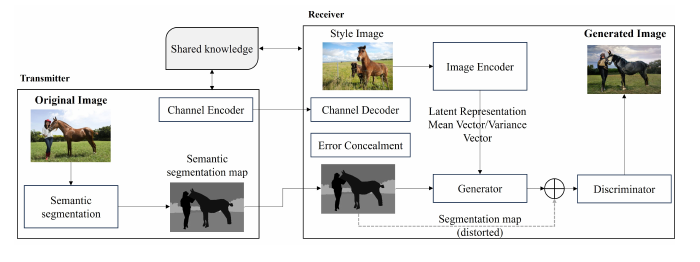
\includegraphics[width=\linewidth]{fig/fig5.png}
\caption{GAI를 갖춘 추론 기반 SC의 구조 [93].}
\label{fig:5}
\end{figure}

VAE에서는 입력 데이터를 한 번의 추론으로 압축하고 복원하므로, 지연이 짧아야 하고 대역폭이 제한된 SC에 적합하다.
잡음에 강한 마스크드(masked) VQ-VAE 체계 [88]는 송신기와 수신기가 이산 부호책을 공유해 의미 잡음을 억제하고 대역폭 사용을 줄인다.
VQ-VAE-2 [98]를 채택한 배포 후 미세 조정 가능 SC(FTSC, post-deployment fine-tunable SC) 체계 [89]도 제안되었다.
FTSC 체계에서는 복호기에서 미세 조정을 거쳐 미지의 데이터 분포에 적응함으로써 일반화 성능을 높일 수 있다.
그러나 VAE에 내재한 저차원 병목은 출력 해상도를 제한한다. 이 단점은 채널 잡음이 클 때 더 심해져 세밀한 의미 정보가 손실된다.

GAN 모델은 전송 강건성 [90], [91]과 의미 충실도 [92], [93]를 높이는 데 쓰였다.
예를 들어 텍스트 입력을 위한 GAN 기반 SC 체계가 제안되었다 [90].
이 체계는 의미 전송을 위한 부호기-복호기와, CSI 없이 왜곡을 완화하는 GAN 기반 모듈을 통합한다 [90].
또 다른 연구는 중요 영역을 보존하기 위해, 관심 영역(ROI, regions of interest)과 비관심 영역(RONI, regions of non-interest)에 기반한 내용 인식 양자화를 GAN과 통합해 적용했다 [91].
이 체계에서는 다중 스케일 GAN 판별기와 무작위 SNR 샘플링으로 열악한 채널에서도 강건성을 얻을 수 있다.
내용 인식 특징만 전송하고 수신기가 GAN으로 고해상도 이미지를 복원하는 SC 방법 [92]도 제시되었다.
마찬가지로, 그림~5에 보인 것처럼 의미 분할된 이미지만 전송해 수신기에서 이미지를 복원하는, SC 방법을 결합한 GAN 모델이 제안되었다 [93].
부분 입력에서 원본 데이터를 추론하는 이 두 방식은 부분적인 의미 입력으로부터 시각적으로 그럴듯한 내용을 재생성하므로 전송 오버헤드를 크게 줄일 수 있다.
그러나 지각적 타당성이 과업 충실도를 보장하지는 못하며, 분포 변화에 취약하다는 점 때문에 동적 무선 환경에 실제로 배포하기 어렵다.

확산 모델은 채널 손상에 대한 강건성을 높이기 위해 SC에 적용되었다.
예를 들어 채널 잡음을 완화하기 위해 채널 잡음 제거 확산 모델 [94]이 도입되었다.
마찬가지로 이미지 전송에 확산 확률 모델(DPM, diffusion probabilistic model)을 적용한 확산 SC(DiffSC, diffusion SC) 체계 [95]도 도입되었다.
이러한 장점에도 불구하고, 확산 모델은 반복적으로 동작하므로 지연 문제가 생긴다.
이 문제를 해결하기 위해 허용할 만한 품질을 유지하면서 샘플링 단계 수를 줄이는 SC 방법 [96]이 제안되었다.
비슷한 맥락에서 Grassucci 등 [97]은 자원이 제한된 환경을 위한 경량 확산 모델을 제안해, 수신기의 계산 오버헤드와 에너지 소비를 모두 줄였다.

SC에서 이 세 가지 생성 모델은 저마다 뚜렷한 강점과 한계가 있다.
VAE, GAN, 확산 기반 방법은 각각 저지연 채널, 대역폭이 제한된 채널, 심하게 손상된 채널에 맞게 구현할 수 있다.
그러나 각 방식에는 VAE의 부호책 동기화, GAN의 지각-의미 불일치, 확산 모델의 샘플링 지연처럼 실용상의 한계가 있다.

\subsection{이질성을 다루는 의미 통신}

앞의 절들은 SC 시스템의 추론 메커니즘에 초점을 두었다.
이 절에서는 추론 능력을 이종 네트워크 시나리오에 적용하는 방안을 살펴본다.

\paragraph{1) NOMA}
기존 연구의 상당수가 단일 사용자 SC에 집중했지만, 몇몇 연구는 이를 다중 사용자 환경으로 확장하는 방안을 탐구했다.
비직교 다중 접속(NOMA, non-orthogonal multiple access)은 전력 다중화로 같은 시간-주파수 자원 안에서 동시 접속을 가능하게 하므로, 다중 사용자 환경의 SC에 적합하다고 여겨진다.
[99]에서는 학습된 이산 표현과 다중 사용자 검출용 신경망을 써서 이종 사용자 데이터 형식을 지원하는 NOMA 기반 SC(NOMASC)를 제안했다.
또한 원거리장(far-field) 사용자는 SC를 쓰고 근거리장(near-field) 사용자는 기존 비트 기반 통신을 쓰는 NOMA 기반 체계도 도입되었다 [100].
전송 유연성을 더 높이기 위해 NOMA를 변형한 semi-NOMA 방법도 제안되었다 [101].

\paragraph{2) 토큰 통신}
이질성은 사용자 수준을 넘어 전송 데이터의 표현 형태에도 존재한다.
다중 접속 환경의 GSC를 위한 새로운 토큰 통신(TokCom, token communication) 체계가 제안되었다 [102].
이 체계에서 토큰은 미래 무선 네트워크에서 전송되는 의미 내용의 단위 역할을 한다.
TokCom에서는 송신기가 다중 모달 신호의 의미 내용을 부호화하고, 수신기가 맥락 정보를 이용해 이를 복구한다.
그림~6에서 보듯이, 단방향 예측은 과거 토큰을 활용해 저지연 부호화와 변조를 가능하게 한다.
반면 양방향 마스크드 예측은 전체 맥락을 써서 패킷 복구 측면의 정확도를 높인다.
[103]에 따르면 TokCom 패킷이 손상되면 메시지가 불완전해질 수 있다.
의미 오류 정정은 사전 학습된 LLM이 수행하며, 이 LLM은 주변 맥락으로부터 마스크된 단어를 예측한다.
따라서 TokCom 기반 맥락 추론은 재전송 횟수를 줄인다.

\setcounter{figure}{5}
\begin{figure}[htbp]
\centering
\begin{minipage}{0.6\linewidth}
\centering
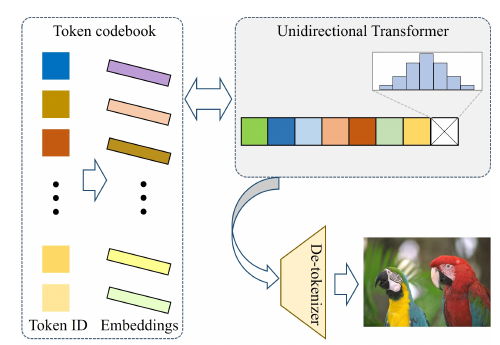
\includegraphics[width=\linewidth]{fig/fig6a.png}\\[2pt]
{\small (a) 단방향 TokCom(다음 토큰 예측)}
\end{minipage}\\[10pt]
\begin{minipage}{0.6\linewidth}
\centering
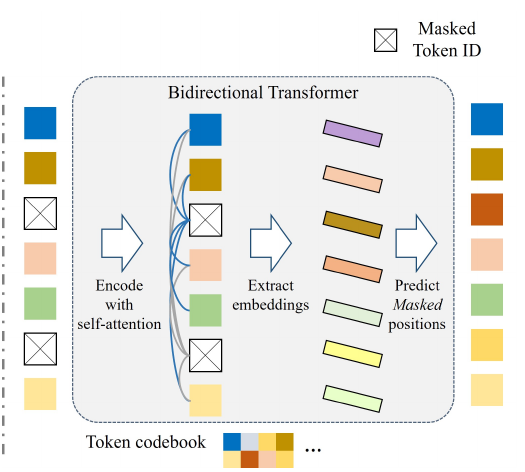
\includegraphics[width=\linewidth]{fig/fig6b.png}\\[2pt]
{\small (b) 양방향 TokCom(마스크드 토큰 예측)}
\end{minipage}
\caption{단방향 TokCom 체계와 양방향 TokCom 체계의 비교 [102].}
\label{fig:6}
\end{figure}

이러한 토큰 기반 통신 패러다임은 학계뿐 아니라 3세대 파트너십 프로젝트(3GPP, 3rd Generation Partnership Project) 같은 표준화 기구에서도 논의되고 있다 [104].
구체적으로 3GPP 시스템 구조(SA, system architecture) 그룹은 패킷이 아니라 \emph{토큰}을 기본 단위로 하여 GAI 서비스를 지원하는 다중 모달리티 트래픽 모델을 정의한다.
또한 이 연구는 토큰 크기, 토큰 중요도 같은 새로운 서비스 품질(QoS, quality of service) 지표를 도입한다.
나아가 Release~19에서는 추론 시간을 핵심 변수로 고려한다 [105].
이러한 흐름은 미래 6G 시스템이 비트 중심의 신뢰성에서 토큰 중심의 의미 신뢰성으로 옮겨 가고 있음을 보여 준다.

\setcounter{table}{7}
\begin{table}[htbp]
\centering
\caption{추론 기반 SC 문헌 검토}
\label{tab:8}
\footnotesize
\renewcommand{\arraystretch}{1.15}
\begin{tabularx}{\linewidth}{|>{\centering\arraybackslash}p{0.2\linewidth}|>{\centering\arraybackslash}p{0.12\linewidth}|>{\centering\arraybackslash}X|}
\hline
\textbf{방식} & \textbf{참고문헌} & \textbf{특징} \\
\hline
\multirow{6}{=}{\centering 맥락적 추론\\(KB 기반)} & [72]--[74] & KG로 개체 관계를 추론해 오류를 정정하고 오버헤드를 줄임 \\
\cline{2-3}
 & [75] & 토큰과 정렬된 KG 개체의 결합 임베딩으로 지식 범위 밖 사례에 대응 \\
\cline{2-3}
 & [44], [76] & KG의 사실 참조와 LLM의 맥락 해석을 결합하는 KG-LLM \\
\cline{2-3}
 & [77] & 사전 학습된 LLM을 암묵적 공유 KB로 사용 \\
\cline{2-3}
 & [78], [79] & 생성 사전 분포를 공유 KB로 써서 과업과 관련된 최소한의 단서만 전송 \\
\cline{2-3}
 & [80] & 텍스트 말뭉치를 읽을 수 있는 KB로 쓰고, 데이터베이스에 없는 과업 관련 정보를 전송 \\
\hline
\multirow{3}{=}{\centering 맥락적 추론\\(인지적)} & [13], [81] & 반복 추론(예: iCR, iLCR)으로 최소한의 비트로 공유 맥락 구축 \\
\cline{2-3}
 & [82]--[84] & 암묵적 구조(예: 인과 그래프)를 전송하고 모방 학습으로 잠재 추론을 재구성 \\
\cline{2-3}
 & [85]--[87] & 과업과 관련된 정보를 선택하고 이종 환경에서 의미 불일치를 완화 \\
\hline
\multirow{2}{=}{\centering 생성형 AI 통합\\(VAE)} & [88] & 공유 부호책을 쓰는 마스크드 VQ-VAE로 잡음 강건성 확보와 중복 억제 \\
\cline{2-3}
 & [89] & 일반화를 높이는 배포 후 미세 조정 가능 VQ-VAE-2 체계 \\
\hline
\multirow{2}{=}{\centering 생성형 AI 통합\\(GAN)} & [90], [91] & 수신 신호의 왜곡을 억제하는 GAN 기반 모듈 \\
\cline{2-3}
 & [92], [93] & 내용 인식 특징을 전송하고 GAN이 고해상도 이미지를 복원 \\
\hline
\multirow{2}{=}{\centering 생성형 AI 통합\\(확산 모델)} & [94], [95] & 반복적 잡음 제거로 채널 잡음을 완화하고 의미를 복원 \\
\cline{2-3}
 & [96], [97] & 단계 수를 줄이거나 경량 모델을 써서 확산의 비용과 지연을 낮춤 \\
\hline
\multirow{2}{=}{\centering 이종 네트워크\\설계} & [99]--[101] & 다양한 데이터 형식과 요구 사항을 위한 NOMA 기반 다중 사용자 SC \\
\cline{2-3}
 & [102], [103] & 내용을 토큰으로 전송하고 LLM이 맥락을 추론해 오류 정정 \\
\hline
\end{tabularx}
\end{table}

\subsection{기존 연구에서 얻은 교훈}

추론 기반 SC는 설계 목표를 특징을 충실히 전달하는 데서, 공유 맥락 안에서 과업을 수행하려면 어떤 정보를 전달해야 하는지 결정하는 쪽으로 옮긴다.
구체적으로 KB 기반 방식은 오류 정정과 맥락 보완을 위한 메커니즘을 제공한다.
PragCom 기반 방법은 화자와 청자의 의도를 모델링해 불필요한 정보 교환을 줄이고, GAI 기법은 직접 전송이 불완전할 때 빠진 의미 내용을 복원하거나 추론한다.

그러나 기존 연구는 충분히 안정적인 의미 기반 위에서만 효과적이다.
그라운딩(grounding)이 약하거나 이질적이면, 추론은 환각이나 조정 오버헤드를 줄이기는커녕 오히려 키울 수 있다.
이 때문에 기존 연구는 추론 복잡도와 성능 향상 사이의 상충 관계에 부딪혀 왔다.
또한 이종 상호 운용성 연구는 의미 시스템과 기존 디지털 시스템이 공존할 수 있음을 보였지만, 의미 비일관성과 표준화된 의미 단위의 부재가 여전히 매끄러운 통합을 가로막고 있다.
추론 기반 SC에 관한 문헌은 표~VIII에 정리했다.

이러한 관찰에서 세 가지 핵심 통찰을 얻을 수 있다.
첫째, 추론은 잠재된 맥락을 명시적으로 드러내 통신을 향상한다.
따라서 송신자와 수신자는 구조화된 지식과 공유 의미 체계로 연결되어 있어야 한다.
둘째, 추론(reasoning)의 효용은 불확실성 감소가 추가 계산 비용을 정당화하는지에 달려 있다. 추론은 기본 추론(inference) 과정을 대체하는 것이 아니라 선택적으로 활용해야 하기 때문이다.
셋째, 진행 중인 3GPP 논의는 미래 6G 네트워크가 의미와 토큰을 인식하는 통신으로 진화하고 있음을 보여 준다.
마찬가지로 AI-RAN Alliance 같은 그룹도 에이전트형 구조를 논의하고 있으며 [106], 이는 통신 시스템이 자율 에이전트 기반 운용으로 옮겨 가고 있음을 뜻한다.
그러므로 다음 진화 단계는 효율적인 추론(inference)과 추론(reasoning), 토큰 중심 통신을 통합하는 에이전트형 체계로 SC를 발전시키는 것이다.

% part_C: 원문 13쪽 "V. AGENTIC SC" ~ 19쪽 V.C 직전 (V.A, V.B), 그림 7--11

\section{에이전트형 의미 통신}

인간의 지각 과정은 선택, 조직화, 해석의 세 단계로 이루어진다 [107].
지각 과정에서 주변 환경의 정보 가운데 일부가 선택적으로 인식되고, 구조화된 표현으로 조직되며, 해석된다.
SC의 발전은 이러한 순차적 인지 과정에 견줄 수 있다.
예를 들어, 선택 단계는 DeepJSCC 같은 직관 기반 의미 통신(intuition-driven SC) 모델이 과업과 관련된 특징을 선택적으로 전송하는 모습으로 나타난다.
그 뒤에 등장한 추론 기반 의미 통신(reasoning-driven SC) 시스템에는 맥락적 추론 모듈이 들어가므로, 이 시스템은 조직화 단계에 해당한다.
이 궤적을 따르면, 다음 진화 단계는 자연스럽게 해석 단계를 겨냥해야 한다.
해석 단계에서는 맥락에 대한 이해와 적응적 추론을 통해 의미가 동적으로 구성된다.
통신 시스템에서 이 해석 단계를 구현하려면, 에이전트는 맥락에서 의미를 추론할 뿐 아니라 통신 제약 아래에서 그 의미에 따라 어떻게 행동할지도 결정해야 한다.

\setcounter{figure}{6}
\begin{figure}[htbp]
\centering
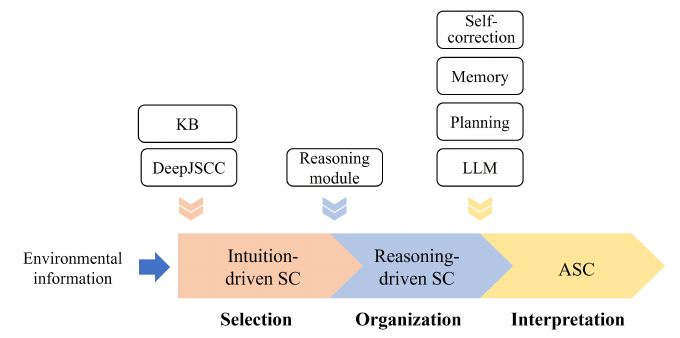
\includegraphics[width=\linewidth]{fig/fig7.png}
\caption{인간의 지각 과정과 의미 통신의 진화 궤적 사이의 개념적 대응.}
\label{fig:7}
\end{figure}

이러한 맥락에서 ASC의 에이전트적 성격은, 정적인 프로토콜에서 벗어나 의미를 추론할 뿐 아니라 협상하기도 하는 동적 상호작용 과정으로 옮겨 가는 것이라고 정의할 수 있다 [108].
LLM은 이러한 창발적 행동을 계산적으로 실현할 수 있게 해 주는 핵심 기술 기반 가운데 하나다.
또한 LLM은 의미 추상화 [109], 맥락적 추론 [110], 처음 보는 입력에 대한 맥락 내 일반화 [110] 능력을 바탕으로 자율적 상호작용을 뒷받침한다.
계획, 메모리, 자기 교정 모듈의 지원을 받으면 LLM은 표현을 발전시키고, 행동의 결과를 예측하며, 전략을 지속적으로 개선할 수 있다.
이러한 메커니즘을 통해 ASC는 에이전트들 사이의 자율적 교환에서 의미가 창발하는 해석 단계를 구현한다.
지각 과정과 의미 통신의 기능 사이의 관계를 그림~7에 나타냈다.

\subsection{ASC의 핵심 구성 요소}

\paragraph{1) 에이전트}
ASC에서 에이전트는 내부 상태와 맥락적 이해를 바탕으로 의미 표현을 생성하고, 해석하고, 발전시키는 데 참여하는 의미적 개체로 본다.
기존 시스템에서 송신기와 수신기는 수동적인 의미 압축기와 압축 해제기로 간주된다.
이와 달리 ASC의 에이전트는 직관과 추론을 모두 아우르는 인지 능력을 갖춘 능동적 참여자로 가정한다.

\paragraph{2) 지각}
ASC 루프는 지각(perception)으로 시작될 수 있다.
지각은 환경 상태를 국소 관측으로 사상하고, 의미 부호기는 이 국소 관측에서 의미 잠재 상태를 추출한다(V-A6절에서 정식화한다).
지각된 의미 잠재 상태는 과업 의도, 메모리, KB 상태, 채널 정보와 함께 무엇을 전송할지에 관한 결정, 전송할 의미, 세계 모델 예측에 의존할지 여부에 영향을 주는 조건이 된다.
따라서 지각은 암묵적 입력이 아니라 명시적인 기능 모듈로 다룰 수 있다.

\paragraph{3) 지식 베이스}
ASC에서 KB는 온톨로지, 제약, 사실, 규칙을 담은 공유 저장소 역할을 하며, 송신기와 수신기가 이를 동적으로 동기화한다고 가정한다 [111].
송신기는 KB를 사용해 원시 데이터를 의미 표현으로 부호화한다 [20].
복호기는 KB를 활용해 낮은 신호 대 잡음비(SNR) 조건에서도 데이터를 강인하게 복원한다.
ASC 프레임워크는 맥락 정보를 부호화하는 데 그치지 않고, KB의 지속적인 갱신과 정렬을 통해 공유되고 구조화된 언어가 동적으로 공진화한다고 가정한다.
상호작용을 통한 이러한 프로토콜 적응은 V-C절에서 논의한다.

\paragraph{4) 세계 모델}
세계 모델은 일종의 꿈 엔진(dream engine)으로 기능한다.
세계 모델 덕분에 에이전트는 미래의 의미 잠재 상태, 곧 미래 환경 상태를 과업에 맞게 추상화한 것을 예측하고, 가능한 행동의 결과를 평가하며, 과업을 실행하기 전에 의사 결정을 뒷받침할 수 있다.
이에 따라 세계 모델은 에이전트가 환경 안에서 자기 행동의 결과를 예측할 수 있게 해 준다 [112].
체화 AI(embodied AI)와 로봇공학 분야에서는 세계 모델이 일관된 미래 예측을 바탕으로 감각운동 제어와 추론을 연결하여, 분포 밖(OOD) 상황에 대한 강인성을 높일 수 있음이 입증되었다 [113].
Ha와 Schmidhuber [112]는 세계 모델 기반 파이프라인을 제시하고, 구성된 ``꿈'' 환경에서 학습한 정책을 실제 환경으로 옮길 수 있음을 보였다.
컴퓨터 비전 분야에서는 비디오 시퀀스를 예측하여 물리적 동역학을 포착하는 WorldDreamer [114]가 제안되었다.

ASC 안에서 세계 모델은 송신기 쪽에서 \textit{의미 상태 기술자(semantic state descriptor)} 역할을 할 수 있다.
이 구성 요소는 숨은 동역학을 추론하여 의미 정보를 효율적으로 부호화할 수 있게 한다.
수신기 쪽에서는 세계 모델을 \textit{청자 의미 추론(listener semantic inference)}으로 구현한다.
이 구성 요소는 복원된 의미 잠재 상태 위에서 이루어지는 후속 기호 추론을 뒷받침하여 과업을 더 효과적으로 수행한다.
이러한 메커니즘을 통해 세계 모델은 에이전트가 이미 확립된 개념을 활용해 처음 보는 시나리오에서도 합리적인 결정을 내리게 해 준다.

세계 모델은 전송 효율과 추론 측면에서 ASC 프레임워크를 강화할 수 있다.
세계 모델은 과업 보상에 따라 중간 추론 상태를 생성하여 행동 공간의 불필요한 탐색을 줄이는 데 쓰였다 [115].
또한 압축에 쓰일 때 세계 모델은 원시 관측 대신 궤적을 예측하여 전송 정보량을 줄인다 [116].
더 나아가, 환경의 구조적 의존성을 학습함으로써 세계 모델을 갖춘 프레임워크는 분포 이동 아래에서도 안정적인 성능을 유지할 수 있다 [43].
이러한 활용은 V-B1절에서 논의한다.

\paragraph{5) 의미 메모리}
맥락 정보를 보강하는 KB와 달리, 의미 메모리(semantic memory)는 전송된 의미 표현(SR, semantic representation)을 저장하고 검색한다.
통신 세션 동안 의미 메모리는 SR을 보관해 뒤이은 패킷 전송에서 다시 사용하며, 이로써 대화의 연속성을 높인다 [117].
의미 메모리는 세션마다 다르며 온라인으로 갱신된다.
맥락 보강과 데이터량 감축을 위한 대표적인 활용 사례는 V-B3절에서 살펴본다.

\paragraph{6) ASC의 수학적 추상화}
여기서는 ASC의 통신 과정과 추론 과정을 수학적으로 추상화하여 기술한다.
정식화에는 관측, 의미 잠재 상태, KB, 세계 모델, EmLang 토큰, 채널 상태, 과업 효용이 포함된다.
이 요소들을 바탕으로 ASC 에이전트는 \textit{어떤} 의미 정보를 전송할지, \textit{언제} 전송할지, 수신한 정보를 추론이나 추리에 \textit{어떻게} 사용할지를 결정한다.
먼저 ASC 에이전트의 기능적 구조를 정의한 뒤, 세계 모델 기반 송수신기 상호작용을 예로 들어 기술한다.
이 추상화의 목적은 유일한 시스템 모델을 규정하는 것이 아니라, ASC의 통신과 추론의 바탕에 있는 기능적 역할과 가정을 밝히는 데 있다.

인터페이스 공간, 내부 상태 공간, 기능 모듈, 결정 계층을 구분하기 위해 ASC 에이전트 $i$를 다음과 같이 나타낸다.
\begin{equation}
\mathcal{A}_i = (\mathcal{I}_i,\, \mathcal{Z}_i,\, \mathcal{M}_i,\, \mathcal{D}_i), \tag{1}
\end{equation}
여기서 $\mathcal{I}_i = (\mathcal{O}_i, \mathcal{U}_i, \mathcal{L}_i, \mathcal{C}_i, \mathcal{R}_i)$는 인터페이스 공간을 모은 것으로, 국소 관측 공간 $\mathcal{O}_i$, 국소 행동 공간 $\mathcal{U}_i$, 의미 토큰 공간 $\mathcal{L}_i$, 채널 상태 공간 $\mathcal{C}_i$, 통신 자원 행동 공간 $\mathcal{R}_i$로 이루어진다.
$\mathcal{Z}_i = (\mathcal{S}_i, \mathcal{H}_i, \mathcal{K}_i)$는 내부 상태 공간을 모은 것으로, 의미 잠재 공간 $\mathcal{S}_i$, 내부 상태 공간 $\mathcal{H}_i$, 국소 KB 상태 공간 $\mathcal{K}_i$로 이루어진다.
$\mathcal{M}_i = (P_i, E_i, \mathcal{W}_i)$는 기능 모듈을 모은 것으로, 지각 함수 $P_i$, 의미 부호기 $E_i$, 그리고 (2)의 세계 모델 모듈 $\mathcal{W}_i$로 이루어진다.
$\mathcal{D}_i = (\pi_i, J_i)$는 결정 계층으로, (3)의 결합 행동-통신 정책 $\pi_i$와 $\pi_i$가 최대화하는 과업 수준 효용 $J_i$로 이루어진다.
이 묶음들은 필수 구성 요소가 아니라 분석상의 역할로 해석해야 한다.
예를 들어 예측 모델링을 쓰지 않는 ASC 구현은 $\mathcal{W}_i$를 생략하거나 다른 것으로 바꿀 수 있다.

\textit{상태 표기.}
환경 상태는 물리적 환경의 실제 상태로 정의한다.
지각 함수 $P_i$는 이 상태를 국소 관측 $o_i^t$로 사상하고, 의미 부호기 $E_i$는 이 관측에서 의미 잠재 상태 $s_i^t = E_i(o_i^t, k_i^t)$를 추출한다.
의미 잠재 상태는 과업과 관련된 간결한 표현이다.
내부 상태는 의미 메모리와 관측 이력을 요약한다.
KB 상태 $k_i^t$와 $k_j^t$는 국소 지식 상태를 나타내며, 특정 구현이 공유 KB에 의존할 때 동기화된다.
채널 상태는 링크 조건을 기술한다.
신념 상태(belief state)는 다중 에이전트 조정을 고려할 때만 도입한다.
따로 밝히지 않는 한, 이 정식화의 나머지 부분에서 ``상태''는 의미 잠재 상태를 가리킨다.

통신과 추론을 결합하는 데 예측을 사용하는 ASC 구현을 생각하자.
에이전트 $i$는 다음 의미 잠재 상태를 다음과 같이 예측한다.
\begin{equation}
\hat{s}_{i,t+1} = \mathcal{W}_i(s_{i,t},\, u_i^t;\, k_i^t), \tag{2}
\end{equation}
여기서 $t$는 이산 시간 슬롯 인덱스, $s_{i,t}$는 현재 의미 잠재 상태, $u_i^t$는 제어 행동, $k_i^t$는 국소 KB 상태다.
예측한 다음 상태 $\hat{s}_{i,t+1}$은 추론을 위한 의미적 사전 정보(semantic prior)로 쓰인다.

송신기 $i$에서 수신기 $j$로 가는 통신 링크에서, 송신기는 내부 상태 $h_i^t$, KB 상태 $k_i^t$, 채널 상태 $c_{ij}^t \in \mathcal{C}_i$를 고려하여 무엇을 전송하고 자원을 어떻게 할당할지 선택한다.
전송 시점은 아래에서 따로 구체화한다.
구체적으로, 송신기는 결합 정책을 통해 제어 행동 $u_i^t$, EmLang 토큰 시퀀스 $\ell_{i\to j}^t \in \mathcal{L}_i$, 자원 벡터 $\rho_{ij}^t \in \mathcal{R}_i$를 다음과 같이 선택할 수 있다.
\begin{equation}
(u_i^t,\, \ell_{i\to j}^t,\, \rho_{ij}^t) \sim \pi_i(\cdot \mid h_i^t, k_i^t, c_{ij}^t). \tag{3}
\end{equation}
전송 결정 $a_{ij}^t \in \{0,1\}$은 (3)의 정책이 출력하는 값이 아니다.
이 값은 아래 (4)의 결정론적 사건 트리거로 정해진다.
이 트리거는 \textit{언제} 전송할지를 정하는 한 가지 구현일 뿐이며, 다른 ASC 설계에서 학습 기반 또는 규칙 기반 전송 결정을 쓰는 것을 배제하지 않는다.
또한 자원 벡터 $\rho_{ij}^t$는 자원 요청(예: 원하는 전송률과 의미적 우선순위)으로 해석하며, 하위의 매체 접근 제어(MAC) 스케줄러가 이를 물리 무선 자원에 사상한다.

세계 모델 기반의 경우에서 \textit{언제} 전송할지의 결정을 명시적으로 만들기 위해, 예측한 의미 잠재 상태와 관측한 의미 잠재 상태 사이의 불일치로 통신을 트리거할 수 있다.
슬롯 $t$ 안에서 제어 행동 $u_i^t$를 먼저 적용하고, 그다음 새 관측에서 의미 잠재 상태 $s_{i,t+1}$을 추출한다.
다음과 같이 정의한다.
\begin{equation}
\epsilon_{i,t} = d_s(s_{i,t+1}, \hat{s}_{i,t+1}), \qquad
a_{ij}^t =
\begin{cases}
1, & \epsilon_{i,t} \ge \epsilon_{\mathrm{th}},\\
0, & \text{그 외},
\end{cases} \tag{4}
\end{equation}
여기서 $\epsilon_{\mathrm{th}}$는 건너뛰기 임곗값이고, $d_s(\cdot,\cdot)$는 의미 잠재 공간에서 정의한 과업 의존 불일치 척도다.
잠재 표현이 유클리드 기하를 허용하면 유클리드 거리를 한 가지 선택으로 쓸 수 있다.
여기서 $a_{ij}^t = 1$은 에이전트 $i$에서 에이전트 $j$로 의미를 전송함을 나타내고, $a_{ij}^t = 0$은 의미를 전송하지 않음을 나타낸다.
(4)의 사건 트리거는 이 구현의 전송 시점 규칙이다.
(1)의 에이전트 수준 표현을 바꾸지 않고도 학습된 트리거나 과업 특화 트리거로 이를 대체할 수 있다.

전송하지 않는 경우, 예측 오차는 환경을 관측하는 유일한 쪽인 송신기에서 측정한다.
표기를 간단히 하기 위해, 활성 링크 하나만 고려할 때는 $\epsilon_t$를 쓴다.
$a_{ij}^t = 1$이면 토큰 시퀀스 $\ell_{i\to j}^t$는 실제 의미 잠재 상태 $s_{i,t+1}$ 또는 $\hat{s}_{i,t+1}$에 대한 그 잔차를 나타내며, 송신기는 예측 상태와 KB를 맥락 정보로 삼아 토큰을 채널 심볼로 부호화한다.
$a_{ij}^t = 0$이면 의미 페이로드를 전송하지 않는다.

수신기에서는 $a_{ij}^t = 1$일 때 성공적으로 복호한 토큰으로 사후 잠재 상태를 $\tilde{s}_{j,t+1} = \phi_j(\hat{\ell}_{i\to j}^t, k_j^t)$로 갱신한다.
그렇지 않으면 수신기는 자신의 국소 예측, 곧 $\tilde{s}_{j,t+1} = \hat{s}_{j,t+1}$을 사용한다.
$a_{ij}^t = 1$일 때의 채널 신뢰도를 $q_{ij}^t \in [0,1]$이라 하고, $a_{ij}^t = 0$일 때는 $q_{ij}^t = 1$로 둔다.
전송하지 않는 경우에 $q_{ij}^t = 1$로 두는 것은, 의도적인 건너뛰기를 수신기가 식별할 수 있다고 가정하는 것이다.
예를 들어 가벼운 1비트 건너뛰기 표시나 미리 합의한 전송 일정을 통해 식별하면, 건너뛰기를 패킷 손실과 혼동하지 않는다.

수신기는 전환 함수를 통해 의미 상태 불일치와 채널 불확실성을 결합할 수 있다.
\begin{equation}
\xi_{ij,t} = \Gamma\bigl(\epsilon_{ij,t},\, 1 - q_{ij}^t\bigr), \tag{5}
\end{equation}
여기서 $\epsilon_{ij,t} = d_s(\tilde{s}_{j,t+1}, \hat{s}_{j,t+1})$는 $a_{ij}^t = 1$일 때 사후 잠재 상태와 국소적으로 예측한 잠재 상태 사이의 불일치를 나타낸다.
함수 $\Gamma(\cdot,\cdot)$는 예측 불일치와 채널 불확실성을 추론 전환 점수로 사상한다.
간단한 가중합 구현은 $\Gamma(\epsilon, 1-q) = \epsilon + \lambda(1-q)$이며, $\lambda \ge 0$이 채널 불확실성의 영향을 조절한다.

$a_{ij}^t = 0$이면 수신기는 이 오차를 국소적으로 측정할 수 없으므로, 보수적인 대리값 $\epsilon_{ij,t} = \epsilon_{\mathrm{th}}$로 대신한다.
이 값은 (4)에서 송신기가 측정한 오차의 상한이다.
이 근사는 송신기와 수신기의 세계 모델이 동기화되어 있다고 가정한다.
이에 따라 전환 임곗값은 $\Gamma(\epsilon_{\mathrm{th}}, 0) < \xi_{\mathrm{th}}$가 되도록 정한다.
그러면 채택한 대리값 아래에서 의도적인 건너뛰기는 시스템 1(System 1) 경로를 따른다.
수신기 출력은 다음과 같다.
\begin{equation}
\hat{x}_j^t =
\begin{cases}
f_{\mathrm{S1}}(\tilde{s}_{j,t+1},\, k_j^t), & \xi_{ij,t} < \xi_{\mathrm{th}},\\
f_{\mathrm{S2}}(\tilde{s}_{j,t+1},\, k_j^t,\, \hat{s}_{j,t+1}), & \xi_{ij,t} \ge \xi_{\mathrm{th}},
\end{cases} \tag{6}
\end{equation}
여기서 $f_{\mathrm{S1}}$은 빠른 추론 경로, $f_{\mathrm{S2}}$는 추리 경로를 나타낸다.
따라서 시스템 1/시스템 2 전환은 세계 모델 불일치와 채널 불확실성을 모두 반영한다.

\textit{세계 모델 동기화.}
건너뛰기 메커니즘이 작동하려면 송신기와 수신기가 공유된 잠재 기준 상태(latent anchor state)에서 출발해 진화하는 동기화된 세계 모델을 실행해야 한다.
이 동기화를 유지하기 위해 두 종류의 정보를 교환한다.
첫째는 모델 파라미터 갱신으로, 예정된 갱신 단계(예: $T_{\mathrm{model}}$ 슬롯마다)에 낮은 빈도로 동기화하거나, 누적된 파라미터 차이가 허용치를 넘을 때 사건 트리거 방식으로 동기화한다.
갱신 주기는 응용의 시간 척도에 맞추어 정한다.
반면 잠재 기준 상태는 실제 전송이 일어날 때마다 갱신된다.
기준 상태를 갱신할 때마다 관련 제어 행동 $u_i^t$도 함께 전달되므로, 수신기는 건너뛰는 슬롯 동안 송신기와 함께 조건부 세계 모델을 실행할 수 있다.
이때 건너뛰는 동안의 의미 표류(semantic drift)는 하트비트 규칙으로 제한할 수 있다.
예를 들어 최대 $N_{\max}$개의 연속 슬롯을 건너뛴 뒤에는 송신기가 $\epsilon_{i,t}$와 상관없이 현재 의미 잠재 상태를 전송한다.
이러한 동기화 조건은 예측 기반 건너뛰기에서 생기는 것이며, 동기화된 수신기 측 예측기에 의존하지 않는 구현에는 필요하지 않다.

\textit{의도 정렬.}
$g_i^t = \psi_i(h_i^t)$와 $\hat{g}_{j\leftarrow i}^t = \varphi_j(\tilde{s}_{j,t+1},\, h_j^t)$가 각각 송신기 $i$의 과업 의도와 수신기 $j$가 추론한 의도를 나타낸다고 하자.
여기서 $\psi_i(\cdot)$와 $\varphi_j(\cdot)$는 과업 의존 사상이다.
의도 수준의 의미 정렬은 $A_{ij}^t = \mathrm{sim}(g_i^t, \hat{g}_{j\leftarrow i}^t)$로 정량화할 수 있고, 그 시간 평균 $\frac{1}{T}\sum_{t=1}^{T} A_{ij}^t$는 한 에피소드에 걸친 의도 보존 정도를 평가한다.

\textit{조정 메커니즘.}
다중 에이전트 ASC 시스템에서 각 에이전트 $i$는 과업과 관련된 신념 상태 $b_i^t = B_i\bigl(h_i^t,\, \{\hat{\ell}_{j\to i}^t\}_{j\in\mathcal{N}_i}\bigr)$를 유지한다.
전송 결정을 바탕으로 활성 통신 링크의 집합을 $E_t = \{(i,j) : a_{ij}^t = 1\}$로 정의한다.
그러면 보편적으로 규정된 조정 목표 대신 $\max_{(i,j)\in E_t} d(b_i^t, b_j^t)$와 같은 과업 의존 발산 기준을 통해 의미적 일관성을 유도할 수 있다.

\textit{범위와 한계.}
이 수학적 추상화는 이 서베이에서 다루는 ASC 구성 요소를 정리하고, 이를 통신, 예측, 추론, 결정 과정과 연결하기 위한 공통 표기를 제공한다.
기존 연구는 프레임워크의 서로 다른 부분에 대응시킬 수 있다.
예측적 계획은 세계 모델과 건너뛰기 규칙 (4)에 대응하고(V-B1절), EmLang 기반 방법은 토큰 공간에 대응하며(V-C절), 메모리 기반 방법과 검색 증강 생성(RAG) 기반 방법은 내부 상태와 KB 상태에 대응하고(V-B3절), 다중 에이전트 강화학습(MARL) 기반 접근은 정책에 대응한다(V-E절).
ASC 시스템에 따라 세계 모델, 결정론적 건너뛰기, 공유 KB, 시스템 1/시스템 2 전환이 필요하지 않을 수도 있다.
학습 절차, 동기화 오버헤드, 종단 간 시스템 검증은 이 서베이의 범위를 벗어난다.

\subsection{ASC의 에이전트 수준 자율성}

LLM은 추론 기반 의미 통신 시스템에서 유망한 모델로 활용되어 왔지만 [44], [76], [118], 적응성이 제한적이어서 자율성에 제약이 있다.
또한 LLM을 사용한 상호작용은 시스템에 추가 부담을 준다.
토큰 처리 때문에 에이전트가 한 번의 추론 주기 안에서 활용할 수 있는 시간적·다중 모달 맥락이 제한된다.
따라서 LLM으로 자율성을 구현하려면 계산 효율적인 설계와 함께 동적 계획, 메모리, 자기 교정 능력이 필요하다.
이 구성 요소 전반에 걸쳐 DRL은 ASC 시스템의 자율 적응을 위한 핵심 메커니즘을 제공할 수 있다.
구체적으로, DRL은 세계 모델을 이용한 예측적 계획 [115], 자기 교정 모듈을 이용한 자율적 오류 교정 [119], 다중 에이전트 환경에서의 협력적 정책 최적화 [120]를 돕는다.

\paragraph{1) 세계 모델을 이용한 예측적 계획}
세계 모델은 ASC를 기존 의미 통신 개념과 구별해 주는 핵심 구성 요소 가운데 하나다.
LLM은 과업 특화 학습에는 능숙하지만 복잡한 동역학을 포착하는 데에는 자주 어려움을 겪는다 [115].
세계 모델은 에이전트가 주어진 맥락에서 결과를 시뮬레이션하고 예측할 수 있게 해 주는 내부 인지 모듈로 기능한다.

LLM의 추론 능력과 세계 모델의 예측 능력을 결합함으로써 ASC는 엣지 일반 지능(EGI, edge general intelligence)과 유사한 프레임워크를 구축한다 [121].
그림~8([121]에서 착안)에 보인 것처럼, 세계 모델 기반 ASC 프레임워크는 시뮬레이션과 실행의 역할을 분리한다.
LLM 기반 에이전트로 구성된 \textit{상호작용 프런트엔드(Interaction Frontend)}는 실세계의 지각과 실행을 담당한다.
반면 세계 모델이 구동하는 \textit{인지 백본(Cognitive Backbone)}은 관측을 부호화하여 예측된 의미 잠재 상태를 도출한다.
상태 예측 구성 요소는 (2)에 해당하며, 기대 보상은 예측된 상태 위에서 보조 보상 평가기가 추정한다.
이 보상은 과업 성능을 최대화하는 행동을 선택하기 위한 지침으로 쓰인다.
지각--예측--행동 루프를 통해 에이전트는 전송 전략을 적응적으로 결정한다.
전체 과정은 다음과 같다.
환경 인식, 의미 잠재 상태 추출, 세계 모델 예측, 전송 결정(건너뛰기 또는 전송), LLM 계획과 자원 할당, 공유 KB를 이용한 의미 토큰 생성, 수신기 추론, 그리고 모델이나 KB에 대한 되먹임 기반 갱신을 통한 세계 모델 재동기화다.
이 나열은 한 슬롯 안의 엄밀한 시간 순서가 아니라 한 번의 닫힌 주기에서의 정보 흐름을 기술한다.
(2)의 세계 모델 예측은 계획기(planner)가 선택한 제어 행동을 조건으로 하며, (4)의 전송 결정은 행동이 실행되고 새 의미 잠재 상태가 추출된 뒤에 내려진다.

\setcounter{figure}{7}
\begin{figure}[htbp]
\centering
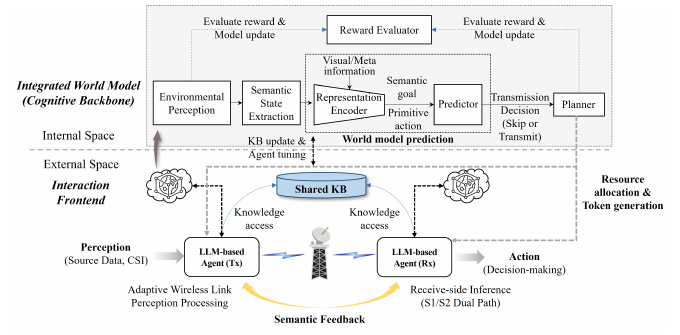
\includegraphics[width=\linewidth]{fig/fig8.png}
\caption{세계 모델 기반 ASC의 폐루프 작업 흐름.}
\label{fig:8}
\end{figure}

세계 모델은 ASC 안에서 두 가지 기능 모듈로 쓰였다.
하나는 통신 인지 동역학 모듈 [115], [122], [123]이고, 다른 하나는 추상화 모듈 [124], [125]이다.
통신 인지 동역학 모듈로 쓰일 때 세계 모델은 미래 행동과 맥락을 고려하여 각 잠재 상태의 효용을 예측한다.
추상화 모듈은 다중 모달 입력을 의미 잠재 상태로 부호화한다.

통신 인지 모듈의 사례로, 최근 연구 [122]는 몬테카를로 트리 탐색을 통합하여 LLM을 세계 모델로 사용한다.
이 프레임워크에서 LLM은 과업 보상의 안내를 받는 추론 트리를 점진적으로 구성한다.
이 방법은 추론 과업에서 사고 사슬(CoT, chain-of-thought) [35] 기준선보다 우수한 성능을 보였다.
또한 LLM은 규칙 학습을 통해 세계 모델로 기능할 수 있다 [123].
에이전트의 궤적을 세계 모델의 예측과 비교함으로써, 이 접근은 기존 에이전트보다 높은 성공률, 빠른 재계획, 낮은 토큰 비용을 달성한다.
이 결과는 LLM 기반 세계 모델이 과업 수준 계획에 효과적일 수 있음을 시사한다.
다만 계산 비용 때문에 시간 제약이 매우 엄격한 통신 루프에서는 여전히 사용이 제한될 수 있다.
이 결과는 [122], [123]에서 일반 추론 벤치마크에 대해 보고된 것이며, 지연 제약이 있는 통신 루프에 적용할 수 있는지는 아직 검증되지 않았다.

세계 모델은 에이전트가 압축된 의미 표현을 전송하게 하여 효율적인 전송을 뒷받침하는 데 쓰일 수 있다.
에이전트는 고차원 정보를 통째로 전송하는 대신, 내부 세계 모델을 사용해 정보를 부호화할 수 있다 [124], [125].
동기화된 세계 모델로 미래 의미 잠재 상태를 예측하고 예측 오차가 임곗값을 넘을 때만 실제 전송을 트리거하면, 전송을 아예 생략할 수도 있다 [116].
이로써 통신 오버헤드, 에너지 소비, 지연이 줄어든다 [116], [124].
더 나아가 세계 모델은 직관적 예측과 논리적 추론을 결합하여 계획을 보완하는 데 쓰일 수 있다 [125].
구현 단계에서 동역학 모듈은 학습된 전이 함수를 사용해 전송 전에 계획을 세운다.
추상화 모듈은 입력을 간결한 잠재 상태로 압축하여 과업이 독립적으로 실행될 수 있게 한다.
수신기의 세계 모델이 충분한 의미 충실도를 갖추면 전송을 건너뛸 수 있다.
이 과정은 V-E절에서 자세히 기술한다.

\setcounter{figure}{8}
\begin{figure}[htbp]
\centering
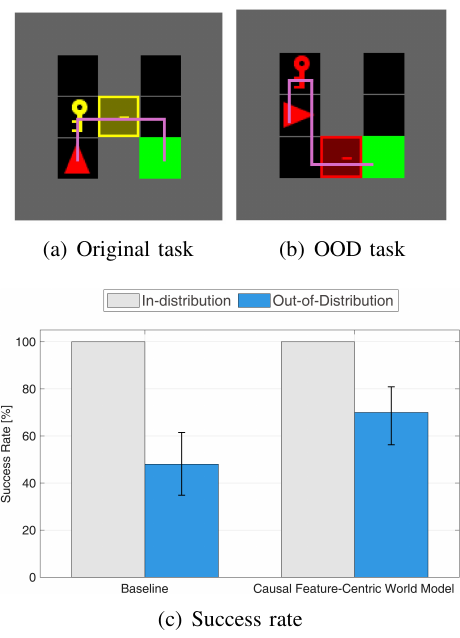
\includegraphics[width=0.6\linewidth]{fig/fig9.png}
\caption{인과적 특징 중심 세계 모델의 OOD 강인성에 대한 시뮬레이션 결과.}
\label{fig:9}
\end{figure}

또한 세계 모델은 OOD 조건에서 성능을 높일 잠재력이 있다.
[43]에서는 세계 모델이 인과적 특징에 집중함으로써 OOD 조건에서 일반화 성능을 높일 수 있음을 증명했다.
다른 연구 [126]은 텍스트 설명을 보조 입력으로 삼아 가려진 영역을 복원하도록 세계 모델을 학습시키면, OOD 조건에서 시각적 변화에 대한 강인성이 향상됨을 보였다.
우리는 OOD 강인성을 평가하기 위해 간단한 시뮬레이션을 수행했다.
[43]을 바탕으로, 열쇠를 사용해 문을 여는 것을 성공으로 정의하는 Minigrid 환경의 DoorKey 과업에서 성능을 평가했다.
OOD 조건을 만들기 위해 문과 열쇠의 색을 바꾸었다.
그림~9에서 대조 손실(contrastive loss)과 정칙화를 사용한 인과적 특징 기반 세계 모델은 기준선보다 높은 강인성을 달성했다.

\paragraph{2) 동적 계획}
앞 소절에서는 잠재적 환경 동역학에 대한 예측적 계획을 다루었다.
이 소절에서는 LLM 중심의 작업 계획과 도구 사용 전략, 곧 추론과 행동(ReAct, reasoning and acting), RAG, 계층적 계획기--실행기 설계에 초점을 맞춘다.

CoT [35]와 사고 트리(tree-of-thought) [36] 같은 핵심 추론 기법은 LLM의 성능을 높이지만 상당한 추론 비용을 수반한다.
또한 LLM의 환각은 신뢰성을 떨어뜨리는 잠재적 위험으로 남아 있다.
정확도, 신뢰성, 효율 사이의 상충 관계를 관리하려면 ASC 시스템은 자율적 추론과 증거 기반 메커니즘을 통합해야 한다.
이러한 맥락에서 ReAct [127]와 RAG [128] 같은 동적 계획 프레임워크는 각각 추론 비용과 환각에 대처하는 실행 가능한 해법이 될 수 있다.
ReAct는 LLM이 외부 도구를 통해 과업을 계획하고 단계별로 행동하게 하여 환각을 효과적으로 완화한다.
RAG는 LLM의 출력을 검증 가능한 외부 지식에 고정하는 메커니즘을 구현한다.
ReAct와 RAG의 개념적 차이를 그림~10에 나타냈다.

\setcounter{figure}{9}
\begin{figure}[htbp]
\centering
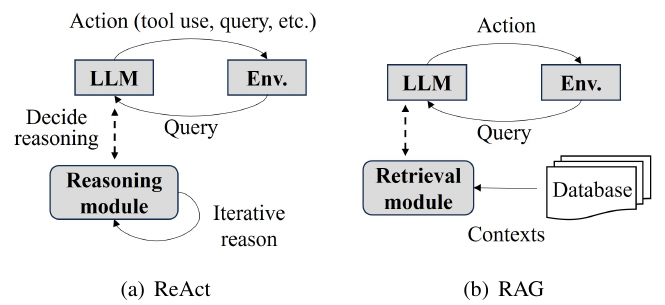
\includegraphics[width=0.85\linewidth]{fig/fig10.png}
\caption{ReAct와 RAG의 개념도.}
\label{fig:10}
\end{figure}

ReAct 원리는 의미 통신으로 확장되었다 [130].
여기서 ASC는 ReAct 메커니즘을 다중 에이전트 계획 프레임워크로 일반화한다.
각 에이전트는 관측을 바탕으로 내부 추론과 외부 실행을 번갈아 수행하며 앞으로의 결정을 반복적으로 다듬는다.
이때 프롬프트 수준의 명시적 추론 흔적은 실제 통신에 필요하지 않으므로 생략한다.
마찬가지로 [129], [131]의 연구는 기존 LLM 기반 방법이 대역폭 할당과 변조 방식을 결합 최적화하지 못함을 보였다.
이 문제를 해결하기 위해, 그림~11에 보인 것처럼 계획 능력을 갖춘 인지 의미 통신 에이전트가 효율적인 자원 할당과 중계기 선택을 가능하게 한다 [129].
더 나아가 과업 계획은 오토인코더 기반 의미 통신이 분포 이동에 민감한 문제를 완화한다 [131].

\setcounter{figure}{10}
\begin{figure}[htbp]
\centering
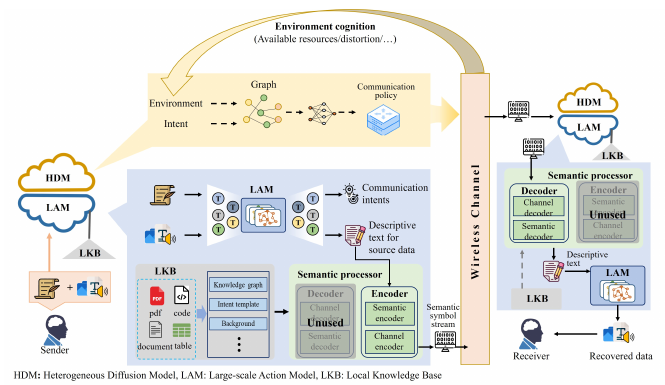
\includegraphics[width=\linewidth]{fig/fig11.png}
\caption{계획 능력을 갖춘 ASC의 프레임워크 예시 [129].}
\label{fig:11}
\end{figure}

RAG는 적응성과 의미적 신뢰성을 높이기 위해 ASC에 적용되었다 [132]--[135].
[132]에서는 검색 증강 다중 모달 의미 통신(RAMSC, retrieval-augmented multimodal SC) 프레임워크를 도입하여, 국소 캐싱과 선택적 검색으로 핵심 다중 모달 요소를 효율적으로 교환할 수 있게 했다.
이를 통해 RAMSC 프레임워크는 정적 검색 방법에 비해 통신 오버헤드를 줄인다.
다른 연구에서는 적용 범위를 넓히기 위해 RAG를 생성형 AI(GAI)와 통합했다 [133].
[133]에 따르면 GAI를 결합한 RAG 방법은 환각 아티팩트를 완화하고 복원 품질을 높인다.
마찬가지로 구조화된 의미 삼중항(semantic triple)과 RAG를 사용하는 개인화 전송 프레임워크 [134]는 의미 콘텐츠 전달의 신뢰성을 한층 강화한다.
통신 시스템에 RAG를 통합함으로써 동적 네트워크의 최적화가 쉬워졌다 [135].
RAG 지식을 활용하면 통신 시스템의 최적화 문제를 자동으로 정식화할 수 있어, 수작업 설계에 비해 모델링 오류가 크게 줄어든다.

RAG는 지식이 보호되는 한 안전한 전송도 보장할 수 있다.
구체적으로, 송신기는 의도한 의미를 나타내는 최소 부분 그래프의 노드 식별자를 전송한다.
수신기는 LLM용으로 생성한 프롬프트를 사용해 자신의 국소 지식 그래프(KG)에서 내용이나 의도를 복원한다 [136].
이 과정은 전송되는 민감 정보의 노출 면을 줄일 수 있다.
그러나 KB에 대한 무단 접근이나 KB의 손상은 정보 유출이라는 새로운 위험을 낳을 수 있으므로, 강건한 정보 보호 전략이 필요하다.
최근 연구 [137]에서는 적대적 학습, 데이터 검증, 이상 탐지 같은 다양한 전략을 사용해 정보 유출이나 조작에 맞서 통신에서 RAG의 보안을 높일 수 있음을 보였다.

LLM을 ReAct나 RAG 방법으로 ASC 프레임워크에 통합하면, 토큰 크기나 처리량과 관련된 통신 오버헤드는 줄지만 추론 지연은 늘어난다.
추론 비용의 균형을 맞추기 위해 ``Plan-and-Act'' [138] 같은 계층적 계획 구조가 등장했다.
이 구조에서 LLM은 상위 수준 계획을 세우는 계획기 역할을 하고, 가벼운 실행기가 그 계획을 효율적으로 실행한다.
``Plan-and-Act'' 개념은 ASC에 Talker--Reasoner 구조로 도입되었다 [37].
이 구조에서 저지연 Talker(시스템 1)는 일반적인 질의를 처리하고, Reasoner(시스템 2)는 불확실성이 높은 상황에서 호출된다.

최근에는 상위 수준의 사용자 의도를 네트워크 구성으로 변환하는 에이전트형 맥락 검색 프레임워크가 제안되었다 [139].
의미 임베딩에 의존하는 RAG 접근과 달리, 이 에이전트형 프레임워크는 다중 출처 지식 검색, CoT 추론, 자기 검증을 통합하여 의사 결정 정확도를 높인다.
그 결과 지능형 기지국은 표준을 준수하는 정책 시행과 관련된 통신 시스템의 복잡한 과업을 자율적으로 수행할 수 있다.

\paragraph{3) 메모리}
ASC 안에서 메모리 모듈은 사용자 행동과 환경 맥락을 비롯해 전송으로부터 얻은 의미 정보를 저장할 수 있다 [140].
또한 최근 연구들은 의미 충실도와 맥락 이해를 높이기 위해 외부 메모리를 도입할 수 있음을 보였다 [117], [141].
구체적으로, 메모리 DeepSC(MeM-DeepSC) [117]는 맥락 정보를 처리하는 메모리 요소를 도입하여, 답변 정확도와 전송 심볼 수 측면에서 기존 의미 통신 모델보다 개선된 결과를 보였다.
메모리를 활용하는 또 다른 방식으로, 확장 맥락 기반 의미 통신은 과거 통신 텍스트라는 개념을 사용한다 [141].
이 의미 통신 프레임워크는 이전에 저장한 문장을 문장 복호 과정에서 추가 맥락으로 재사용하여 정확도를 높였다.

최근 연구들은 맥락 강화보다는 전송 효율을 높이기 위한 메모리 사용을 탐구했다.
진화형 의미 통신 프레임워크 [142]에서는 중복 전송을 피하기 위해 의미 캐싱 전략을 사용한다.
새 의미 벡터가 메모리에 저장된 벡터와 유사하면, 시스템은 일치한 벡터의 인덱스만 전송한다.
또 다른 접근 [143]은 정적 부호책을 갖춘 메모리 기반 분류 모델을 채택한다.
시스템은 가장 가까운 부호책 항목을 선택해 의미 양자화를 수행하고, 해당 인덱스를 전송한다.
이런 방식으로 메모리를 사용하면 학습 오버헤드가 줄고 시간 효율이 높아진다.

\paragraph{4) 자기 교정}
LLM에서 오류를 자율적으로 식별하고 교정하는 능력을 자기 교정(self-correction)이라 한다 [144].
초기 연구는 주로 외부 되먹임 없이 오류를 바로잡는 LLM 고유의 능력에 초점을 맞추었다 [145].
그러나 LLM은 고유 능력만으로는 오류를 교정하는 데 어려움을 겪는다는 사실이 밝혀졌다 [145].
예를 들어 외부 되먹임이 없는 LLM은 올바른 응답을 수정해 버려 성능이 떨어질 수 있다 [146].
이에 따라 후속 연구는 외부 되먹임이나 미세 조정을 통해 자기 교정을 개선하는 데 초점을 맞추었다 [147].
자기 교정 과정에 자기 비판을 통합함으로써 LLM의 정확도가 더욱 향상되었다 [147].

ASC 시스템에서 자기 교정은 에이전트가 자율적으로 개선하는 능력을 가리킨다 [119].
이러한 자기 교정은 에이전트가 자신의 사고 과정을 평가하고 개선하는 능력인 메타인지(meta-cognition)에 해당한다.
의미 오류는 두 유형으로 분류된다.
하나는 가우스 과정 의미 오류이고, 다른 하나는 인간 참여형 강화학습(HITL-RL, human-in-the-loop reinforcement learning) 의미 오류다.
가우스 과정 오류는 잠재 공간에서 이상값으로 식별되며, 데이터 분포 이동, 채널 변동, 적대적 공격 같은 객관적 요인에서 비롯된다 [148].
이와 달리 HITL-RL 오류는 사용자 선호 같은 주관적 변화에서 비롯되며, 인간 되먹임을 활용한 DRL로 바로잡는다 [119].
최근의 발전은 전문가의 도움 없이도 DRL을 통해 자기 교정을 효과적으로 이끌어 내거나 구현할 수 있음을 보여 주었다 [115], [149].

% part_D: 원문 19쪽 V-C 소절 ~ 24쪽 VI절 제목 직전 (그림 12--14, 표 IX--X)
\setcounter{subsection}{2}
\subsection{ASC의 시스템 기반 적응성}

\subsubsection{운영 적응성}
IV절에서 언급했듯이, 모델을 경량화하더라도 추론은 지연과 에너지 소모를 피할 수 없고, 이는 시스템에 부담을 준다. 따라서 ASC 시스템은 과업 성능과 효율의 균형을 맞추는 제어·오케스트레이션 능력을 갖춰야 한다.
대표적인 오케스트레이션 추상화로는 LangChain과 LangGraph가 있으며, 이들은 LLM 기반 구조에서 오케스트레이션 프레임워크로 쓰여 왔다 [150].
오케스트레이터를 쓰는 방식에는 계층형 패턴 [151], [152]과 분산형 패턴 [153]이 있다. 계층형 패턴에 기반한 시스템은 작업 흐름이 명확하지만, 중앙 제어 에이전트가 고장 나면 시스템 전체가 영향을 받을 수 있다. 분산형 패턴은 대등하게 협력하는 에이전트들에 의존한다. 분산형 패턴은 에이전트 고장에 유연하게 대응하지만, 조정이 길어지면서 지연이 생길 수 있다.

의미 통신 시스템에서는 LangGraph 같은 오케스트레이션 기법을 그대로 적용하기에는 계산 부담이 너무 크다. 그래서 의미 통신 시스템 연구는 주로 지능형 스케줄러 역할을 하는 실행 정책 모듈에 초점을 맞춰 왔다. 대표적인 연구 흐름은 의존성 인지 프레임워크를 채택한다. 이 프레임워크에서는 과업 실행을 방향성 비순환 그래프(DAG, directed acyclic graph)로 나타내고, 오프로딩 결정을 MDP로 정식화한다 [154](그림~\ref{fig:12} 참조). 이 프레임워크에서 DRL 에이전트는 지연과 에너지 제약을 함께 고려해, 각 하위 과업을 로컬에서 실행할지 MEC 서버로 오프로딩할지 동적으로 결정한다. 이와 비슷하게, MEC를 활용한 오프로딩을 위한 의미 인지 프레임워크도 제안되었다 [155]. 이 방식은 오프로딩 전에 과업 관련 정보를 압축해 전송 오버헤드를 줄인다. 이러한 연구들은 ASC 환경에서 오케스트레이션 원리가 자원 인지 스케줄러로 재정식화되고 있음을 보여 준다.

\setcounter{figure}{11}
\begin{figure}[htbp]
\centering
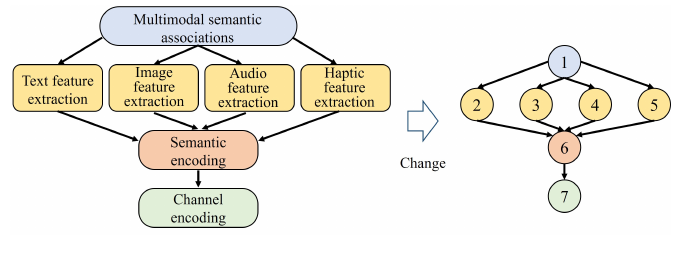
\includegraphics[width=0.8\linewidth]{fig/fig12.png}
\caption{적응성을 위한 ASC 구조 [154].}
\label{fig:12}
\end{figure}

최근의 최전선 에이전트 시스템은 빠른 추론 모드와 깊은 추론 모드 사이를 적응적으로 오가는 라우팅으로 오케스트레이션의 일부를 내재화한다. 한편 새로 등장하는 에이전트 프로토콜은 이종 에이전트 사이의 조정을 지원한다 [156]. ASC에서 이 변화는 적응성의 무게를 과업 스케줄링에서 에이전트 내부의 추론 제어와 에이전트 사이의 의미 조정으로 옮겨 놓는다. 그러나 동기화 오버헤드, 지연, 표준화 문제 때문에 ASC에 대규모 오케스트레이션을 도입하는 일은 여전히 과제로 남아 있다 [153], [157].

\subsubsection{창발적 통신을 통한 프로토콜 적응성}
ASC의 에이전트형 본질은 의미와 전략을 동적으로 조정하는 능력에 있다. 이 적응성은 창발적 통신(EmCom)/EmLang로 구현된다. 여기서 에이전트들은 사람의 개입 없이 에이전트 사이의 지속적인 상호작용을 통해 통신 프로토콜을 스스로 수립하고, 협상하고, 발전시킨다. 의미 통신 밖에서도 프로토콜 적응성은 더 넓은 네트워킹 연구계에서 오랫동안 연구되어 왔다. 예를 들어 DFG 공동연구센터 MAKI는 기능적으로 동등한 프로토콜 메커니즘 사이를 자동으로 전환해, 통신 시스템을 실행 중에 적응시키는 방법을 연구했다 [158]. 이와 달리 EmCom은 프로토콜 적응을 미리 정의된 메커니즘 가운데 하나를 고르는 일에서, 의미적 상호작용을 통해 통신 규칙을 적응적으로 수립하는 일로 확장한다.

AI 에이전트가 사람의 개입 없이 상호작용만으로 프로토콜을 수립할 수 있는지에 대해서는 대중의 관심도 컸다. 특히 ``코드로 소통하는 AI 에이전트''를 담은 영상이 널리 퍼졌는데, 이 영상은 새로운 기계 언어의 출현을 보여 주는 것으로 흔히 오해되었다 [159]. 그러나 실제로 이 영상이 보여 준 것은 GibberLink라는 미리 정의된 프로토콜의 사용이었다 [160]. 이것이 새로운 언어의 출현은 아니었지만, 대중의 반응은 AI 에이전트가 상호작용을 통해 통신 규칙을 만들어 낼 수 있는지에 대한 관심을 드러낸다.

EmLang의 개념적 연구는 Lewis의 신호 게임(signaling game)에 기반한 게임 이론적 틀에 뿌리를 둔다 [161]. 이 모형에서 송신자와 수신자는 신호--의미 관례를 반복적으로 형성하며, 명시적으로 합의하지 않고도 상호 이익을 최대화하는 체계로 수렴한다. 이후 딥러닝과 MARL이 발전하면서 이 신호 게임 패러다임은 신경망 기반 에이전트로 확장되었고, 통신 프로토콜을 자율적으로 형성할 수 있음이 입증되었다 [108].

이론적 실현 가능성은 최근 LLM을 이용한 실험으로 구체적으로 입증되었다. 연구자들 [162]은 무작위로 짝지은 AI 에이전트 24--200개에게 같은 대상에 이름을 붙이게 하는 실험을 했다. 같은 선택에는 보상을, 다른 선택에는 벌점을 주는 간단한 규칙만으로도 에이전트들은 몇 번의 상호작용 만에 공통 기호로 수렴했다. 이 결과는 프로토콜 수준에서 자율적 합의가 가능함을 시사한다. 그럼에도 이 실험은 신뢰할 수 있는 상호작용이라는 맥락에서 고정된 보상 규칙으로 제한되었다. 또한 구문 형성이나 오류 처리처럼 이름 붙이기를 넘어서는 프로토콜 기능은 고려하지 않았다. 구문 형성, 오류 복구, 개방형 환경에서의 상호 운용성 같은 더 복잡한 프로토콜 기능으로 확장할 수 있는지는 여전히 미해결 문제다.

자율적 합의라는 현상을 정식화하기 위해, EmLang·세계 모델·LLM을 잇는 생성적 틀로 집단 예측 부호화(CPC, collective predictive coding)가 제안되었다. CPC에 따르면 언어는 사회 집단 안에서 감각-운동 정보의 예측 가능성을 높이도록 진화했으며, 분산 베이즈 추론으로 모형화된다. 예를 들어 생성적 창발 통신(gEmCom, generative emergent communication) [163]은 CPC 가설에 기반한 생성 모델이다. 많은 EmLang 연구 [164], [165]는 판별적 모델링으로 통신 프로토콜을 최적화하는 데 집중해 왔다. 반면 CPC와 gEmCom은 언어의 출현을 생성 모델에 기반한 추론 과정으로 본다. 따라서 gEmCom 틀에서는 CPC가 언어를 생성하고, LLM은 그 언어로부터 집단 표현을 복원하는 복호기 역할을 한다.

\subsection{ASC의 다중 에이전트 기반 확장성}

\subsubsection{협력 통신과 조정}
ASC를 확장하면 다중 에이전트 통신이 필연적으로 뒤따르며, 이는 다중 에이전트 시스템(MAS) 환경에서 LLM 기반 기술의 발전을 이끈다. 이전의 MAS 연구는 규칙 기반 조정에 초점을 맞췄지만, LLM이 발전하면서 최근에는 자연어를 이용하는 MAS 연구들이 제안되었다.

LLM 에이전트 통신 연구들은 자연어를 넘어서는 공유 상태 표현이 협력 효율을 높일 수 있음을 보여 준다. 예를 들어 ChatDev [152]는 각 단계의 출력을 공유 메모리로 삼아 다음 단계로 넘긴다. 에이전트들이 중간 출력을 공유하면 공통 이해를 형성하고 맥락을 보존할 수 있다. 마찬가지로 Voyager [166]는 에이전트들을 위한 공유 KB 역할을 해, 한 에이전트가 학습한 의미 있는 지식을 다른 에이전트가 활용할 수 있게 하고, 이로써 경험의 공유를 돕는다.

ASC 시스템에서는 협력에 최적화된 공유 표현을 활용해 통신을 원활하게 하는 다양한 방법 [120], [167]--[169]이 제안되었다. 차량 네트워크에서 AI 에이전트는 시각-언어 모델을 이용해 원시 센서 데이터를 간결한 의미 표현으로 변환할 수 있다 [167]. 이 통합 방식은 이종 에이전트들 사이에 환경에 대한 공유된 이해를 촉진할 뿐 아니라, 대역폭 사용과 체감 품질(QoE, quality of experience) 사이의 절충도 최적화한다. 다중 에이전트 지각에서 PragCom은 시공간 희소화, 공유 부호책 압축, 피어 선택을 활용해 고정된 비트 예산 안에서 정확도를 최적화한다 [168]. EmCom에 기반한 협력 방식도 제안되었는데 [120], 여기서 에이전트들은 특정 과업을 풀기 위한 통신 프로토콜을 독립적으로 만들어 낸다. 더 나아가 여러 에이전트에게 통일된 KB가 없다는 문제를 해결하기 위해 명명 게임(naming game)을 활용한 연구가 제안되었다 [169]. 그림~\ref{fig:13}은 MAS의 ASC 구조와 에이전트 사이의 명명 게임 과정을 보여 준다. 이러한 연구들은 잠재 표현을 공유해 협력을 강화하지만, 에이전트들 사이의 합의가 해석 가능성을 해칠 수 있다. 따라서 이종·대규모 환경에서 신뢰할 수 있는 협력을 보장하려면 해석 가능한 표현 학습을 함께 도입해야 한다.

\setcounter{figure}{12}
\begin{figure}[htbp]
\centering
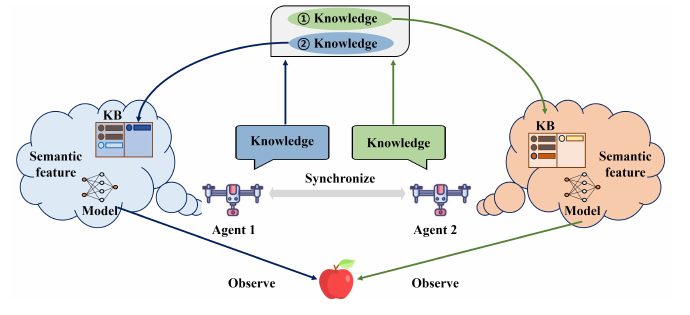
\includegraphics[width=0.8\linewidth]{fig/fig13.png}
\caption{MAS를 위한 ASC 구조 [169].}
\label{fig:13}
\end{figure}

구조화된 데이터를 공유 상태로 활용하는 연구들 [170]--[172]도 제안되었다. 한 연구 [170]에서는 LLM을 공유 KB로 써서 복잡한 데이터를 분할 지도와 경계 상자 같은 구조화된 의미 표현으로 변환하고, 이를 공유해 다중 사용자 협력에 활용했다. [171]에서는 센서가 환경 관측을 공유 격자 세계 지도에 갱신하고, 로봇은 이 지도를 이용해 과업을 수행한다. 화자와 청자가 계층적 신념 집합(hierarchical belief set)이라는 공통 언어로 협력하는 모델도 제안되었다 [172]. 이 모델에서는 단순한 문장 대신 여러 수준으로 추상화된 신념으로 이루어진 구조화된 표현 덕분에 정보를 더 효율적으로 전달할 수 있다. 구조화된 의미 표현을 활용하면 대화형 데이터를 쓸 때보다 과업 관련 정보를 더 효율적으로 교환할 수 있다는 점이 두드러진 장점이다.

\subsubsection{엣지 배포 전략}
AI 기반 네트워크에서는 다층 구조를 구축하기 위해 엣지--클라우드 협력이 구상되어 왔다 [170]. 그러나 자원이 제약된 환경에 에이전트를 배포하는 데에는 계산 능력과 에너지 소비에 관련된 어려움이 따른다. 따라서 이러한 제약 아래에서 동작하려면 ASC 에이전트를 경량화된 형태나 오프로딩되는 형태로 설계해야 한다 [173], [174].

경량 구조는 가지치기, 양자화, 지식 증류를 통해 과업 성능을 유지하면서 모델 복잡도를 줄인다 [173]--[175]. 또한 설계 단계부터 소형 구조를 채택하면 추론 효율을 높일 수 있다. 시스템 1과 시스템 2를 결합한 경량 LLM에 관한 최근 연구 [176]는 과업에 최적화된 초소형 LLM이 기존 구조보다 모델 크기를 크게 줄이면서도 성능을 높일 수 있음을 보여 준다. 이 결과는 ASC 프레임워크가 소규모 LLM으로도 계산 효율과 과업 지향 성능을 달성할 수 있음을 입증한다.

계산 오프로딩은 에이전트 추론을 엣지--클라우드 계층에 분산하는 수단으로 연구되어 왔다 [170]. 모델 분할은 신경망 층을 로컬 기기와 엣지 서버로 나눈다. 이와 달리 시간 분할 복호는 초기 반복을 엣지에서 실행하고 최종 정제는 로컬에서 마무리함으로써, 생성 모델의 부분 오프로딩을 가능하게 한다.

데이터 효율은 과업과 관련된 정보만 선택적으로 전송해 얻는다. 에이전트는 부분 의미 샘플링으로 과업과 관련된 데이터 조각을 전송하고, 수신 측은 이 조각들을 합쳐 과업 지향 복원을 수행한다 [175]. [177]에서는 정보 이득에 따라 의미적으로 중요한 토큰을 선택적으로 보존하는 놀람(surprisal) 유도 압축이 제안되었다. 이 압축을 LLM 기반 에이전트에 적용하면 전송 지연과 에너지 소비를 크게 줄일 수 있다. 모듈형 계층 설계는 과업을 전문화된 에이전트들로 분해한다 [178]. 상위 에이전트는 장기 목표를 다루고, 하위 에이전트는 채널 상태에 맞춰 의미 압축을 조정한다 [178].

\subsection{6G 네트워크에서의 ASC 구현}

\subsubsection{ASC 학습 파이프라인}
앞의 소절들에서는 ASC의 기본 능력들을 소개했다. 이 소절에서는 이를 세 단계로 이루어진 학습 파이프라인으로 묶는다. 세 단계는 (i) MARL 기반 ASC 학습, (ii) OOD 강건성을 위한 세계 모델 시뮬레이션, (iii) 적응적 추론 제어다.

\paragraph{a) MARL 기반 ASC 학습}
첫 단계는 MARL을 통해 ASC 에이전트의 기본 정책을 확립한다. 협력하는 에이전트 $N$개의 집합을 생각하자. 각 에이전트 $i$는 국소 정책 $\pi_{\theta_i}(a_i \mid o_i)$를 유지한다. 이 정책은 에이전트의 국소 관측 $o_i$(예: 원천 데이터의 의미 특징이나 추정된 CSI)를 행동 $a_i$(예: 의미 압축률, 부호책 선택, 전송 여부 결정)로 사상한다.

기존의 비트 수준 목표와 달리, ASC는 과업 수준의 의미 보상을 최적화한다. 시간 단계 $t$에서 각 에이전트의 보상은 다음과 같이 정식화할 수 있다.
\begin{equation}
R_t^i = r_{\mathrm{local}}^i(o_i, a_i) + R_{\mathrm{cluster}}(\bm{\tau}, \mathbf{a}) - c_i(o_i, a_i), \tag{7}
\end{equation}
여기서 $\mathbf{a} = (a_1, \ldots, a_N)$은 결합 행동이고, $\bm{\tau} = (\tau_1, \ldots, \tau_N)$은 결합 행동-관측 이력이다. 하류 의미 과업에 대한 각 에이전트의 개별 기여는 $r_{\mathrm{local}}^i$로 정량화하고, $c_i$는 에이전트의 전송 오버헤드다. $R_{\mathrm{cluster}}$는 협력 과업 성능을 반영하며, 에이전트들이 자신의 표현을 공유 프로토콜에 정렬하도록 유도한다. 이로써 명시적인 지도 없이도 과업에 최적화된 통신 언어가 창발한다.

6G의 대규모 엣지 환경을 고려하면, 중앙집중 학습·분산 실행(CTDE, centralized training with decentralized execution)이 적절한 선택이다. 이 틀을 지원하기 위해, 다중 에이전트 학습에서 확장성과 안정성을 갖춘 다중 에이전트 근접 정책 최적화(MAPPO, multi-agent proximity policy optimization)\onote{MAPPO의 원래 명칭은 multi-agent \emph{proximal} policy optimization이다.}를 구현한다. MAPPO는 전역 상태 $s$에서 평가되는 중앙집중 비평자 네트워크 $V_\phi(s)$를 쓴다. 분산된 각 행위자는 다음의 절단 대리 목적함수(clipped surrogate objective)를 최대화하도록 자신의 정책을 갱신한다.
\begin{equation}
L(\theta_i) = \E\Big[\min\Big(\rho_i \hat{A}_i,\, \mathrm{clip}(\rho_i, 1-\epsilon, 1+\epsilon)\hat{A}_i\Big)\Big], \tag{8}
\end{equation}
여기서 $\rho_i$는 정책 비율이고, $\hat{A}_i$는 중앙집중 비평자가 추정한 어드밴티지다.

\paragraph{b) OOD 강건성을 위한 세계 모델 시뮬레이션}
OOD 상황에서 모델의 강건성을 높이기 위해 세계 모델을 쓴다. 이 모델은 MARL 학습 과정에서 얻은 궤적을 바탕으로 환경의 동역학을 예측하도록 구축된다. 환경으로부터 동역학을 학습한 세계 모델은 동적 계획 과정 $H$에 걸쳐 합성 롤아웃을 생성할 수 있다. 또한 세계 모델은 송신기에서 추상화 모듈 역할도 한다. 즉 원시 고차원 관측을 그대로 전송하는 대신, 다중 모달 입력을 간결한 의미 잠재 상태로 부호화한다.

각 에이전트는 합성 궤적을 이용해 다음과 같이 정책을 갱신한다.
\begin{equation}
\theta_i \leftarrow \theta_i + \alpha\, \nabla_{\theta_i} \E_{\hat{T},\, \pi_{\theta_i}}\left[\sum_{\tau=t}^{t+H} \gamma^{\tau-t} \hat{R}(\hat{s}_\tau, \hat{a}_\tau)\right], \tag{9}
\end{equation}
여기서 $\alpha$는 학습률이고 $\gamma$는 할인 인자다. 이 모델 기반 갱신 덕분에 에이전트는 원래라면 대규모 탐색이 필요했을 일반화 능력을 얻을 수 있다 [43]. 모델은 또한 분포 불일치의 정도를 반영하는 예측 오차 $\epsilon_t$(V-A6절에서 정의)를 출력한다. $\epsilon_t < \epsilon_{\mathrm{th}}$이면 수신기의 세계 모델이 과업 수행에 충분한 의미 충실도를 유지하므로 전송을 건너뛸 수 있다. 그렇지 않으면 재계획이나 전송을 실행한다 [116].

\paragraph{c) 적응적 추론 제어}
배포 단계에서 에이전트는 실시간 지연·에너지 예산 안에서 동작해야 한다. 이 요구를 충족하기 위해, ASC의 마지막 단계는 시스템 1/시스템 2 틀 [35]에서 착안한 이중 모드 추론 메커니즘을 쓴다. 시스템 1은 과업에 최적화된 소형 LLM이나 MARL 정책에 의존해 일상적인 통신 과업을 처리한다. 시스템 2는 복잡하거나 낯선 상황에서 세계 모델 계획기와 함께 추론 파이프라인을 가동한다.

두 모드 사이의 전환은 (5)의 전환 변수가 제어하며, 이 변수는 (6)의 규칙을 따른다. 예측 오차 $\epsilon_t$는 현재 관측이 얼마나 예상 밖인지를 정량화하는 놀람 신호로 해석할 수 있고, 따라서 에이전트의 토큰화와 전송 결정을 내리는 데 도움을 준다. 에이전트는 기본적으로 시스템 1을 쓰고 필요할 때만 시스템 2를 호출함으로써, 과업 성능을 유지하면서 추론 지연과 에너지 소비를 줄인다.

6G 구조에서 이 세 단계는, O-RAN 기반 배포의 한 후보로서, II절에서 설명한 RIC 제어 계층에 대응시킬 수 있다. MARL 기반 학습과 세계 모델 학습은 비실시간 RIC에 rApp으로 배치하며, 그 제어 루프는 1초보다 긴 간격으로 동작한다. 반면 적응적 추론 제어는 준실시간 RIC에서 xApp으로 실행하며, 그 제어 루프는 10~ms에서 1~s 정도의 간격으로 동작한다 [179]. 시스템 2 추론이 이 예산을 넘기면, 현재 결정은 시스템 1이 내리고 시스템 2의 결과는 나중에 비동기 정책 갱신으로 반영한다. 이 대응은 경량 예측 제어기를 xApp으로 배포하고 LLM 기반 의도 변환기를 rApp으로 운용한 최근 구현 [28]과도 일치한다. 이렇게 얻은 정책과 모델 갱신은 비실시간 RIC에서 준실시간 RIC로 A1 인터페이스를 통해 전달되며, A1 인터페이스는 정책 관리와 ML 모델 관리 서비스를 제공한다 [179].

\subsubsection{ASC의 지원, 모니터링, 최적화}
앞서 설명한 O-RAN 대응은 ASC 기능을 배치하는 한 가지 방법을 보여 준다. 기능 배치를 넘어 ASC를 실현하려면 과업 인지 네트워크 지원, 모니터링, 폐루프 최적화가 필요하며, 이를 아래에서 논의한다. 이에 따라 6G 네트워크는 데이터 중심 자원 관리에서 통신·컴퓨팅·에이전트 상호작용의 과업 인지 오케스트레이션으로 진화해야 한다.

\paragraph{a) ASC 지원}
ASC는 과업 수준과 에이전트 수준의 정보를 고려함으로써 기존 네트워크 제어·관리를 확장한다. 3GPP TR 22.870은 AI 서비스와 AI 에이전트 사이의 통신을 위한 6G 활용 사례와 서비스 요구 사항을 다루며 [180], ITU-T 권고는 ML 파이프라인과 그 관리·오케스트레이션을 위한 구조적 틀을 제시한다 [181]. ASC에서는 의도, 의미 우선순위, 추론 마감 시한, 모델 또는 KB 식별자 같은 정보를 권한 있는 네트워크 제어 기능에 제공해 통신·컴퓨팅 자원 할당에 쓸 수 있다. 6G의 핵심 방향은 과업 의도와 에이전트 능력을 네트워크 제어에 반영해, 통신과 에이전트 상호작용을 과업 요구 사항에 따라 관리할 수 있게 하는 것이다.

\paragraph{b) ASC 모니터링}
네트워크 데이터 분석과 폐루프 제어 관리를 위한 기존 3GPP 메커니즘을 ASC 모니터링의 기반으로 적용할 수 있다 [182], [183]. 기존 네트워크 텔레메트리에 더해 과업 진행도, 추론 지연, 에이전트 가용성, 모델 또는 KB 일관성도 고려할 수 있다. 궁극적으로 ASC 모니터링은 네트워크 상태와 에이전트-과업 상태를 함께 볼 수 있게 해서, 통신 실패를 추론·지식·조정 실패와 구별할 수 있게 해야 한다.

\paragraph{c) ASC 최적화}
모니터링한 정보를 바탕으로, 네트워크 제어기와 에이전트 제어기는 폐루프 제어를 통해 통신, 계산, 에이전트 조정을 적응시킬 수 있다. 이에 해당하는 결정에는 전송과 스케줄링, 추론 배치, 피어 선택, 모델 또는 KB 동기화가 있다. 이러한 결정은 지연, 신뢰성, 에너지, 프라이버시, 컴퓨팅 제약을 고려하면서 과업 효용에 따라 최적화할 수 있다 [184]. 더 넓게 보면, ASC 제어는 통신·컴퓨팅·에이전트 상호작용이 바탕 과업의 진행과 성능에 기여하는 정도에 따라 이들을 조정해야 한다.

\subsubsection{ASC의 6G 프로토콜 스택 통합}
다음으로 6G 배포를 위해 알고리즘 수준의 통합에서 프로토콜 스택 수준의 통합으로 넘어간다. 의미 통신을 기존 계층형 스택에 통합하려는 최근 시도는 크게 두 방향에 집중해 왔다. 첫째 접근 [185], [186]은 호환성을 유지하기 위해 의미 통신 기능을 기존 프로토콜 스택에 대응시킨다. 둘째 접근 [187], [188]은 의미 추출, 맥락 추론, 과업 인식 최적화에 초점을 맞춰 계층 구조를 재설계한다. 구체적으로, 전자는 기존 PHY/MAC 스택을 수정하지 않고 전송 계층 위에 의미 기능을 둔다. 후자는 프로토콜 스택을 재구성해 전용 의미 계층을 도입한다. 이 서베이 전체에서 쓰는 계층 할당은 이 소절의 끝에서 설명한다.

프로토콜 스택의 하드웨어 교체 비용과 시스템 복잡도를 줄이기 위해, 개방형 시스템 상호 연결(OSI, open systems interconnection) 모델의 응용 계층 안에 의미 부계층을 결합하는 통합 방법이 제안되었다 [185]. 또한 기존 5세대(5G) 프로토콜 스택과 상호 운용되는 별도의 의미 기반(Seb, semantic-base) 프로토콜 스택도 제안되었다 [186]. 이러한 상호 운용형 접근은 기존 인프라와 점진적으로 통합하기 쉽게 해 주지만, 계층 간 처리 지연과 헤더 추가 때문에 오버헤드가 불가피하게 생긴다.

기존 프로토콜 스택을 의미 통신에 맞춘 3계층 모델로 재편한, 지능적이고 효율적인 의미 통신 구조가 제안되었다 [187]. Fleming 등은 OSI 모델에 새로운 계층 두 개를 추가할 것을 제안한다 [188]. 추가된 계층은 확장 가능한 분산 에이전트 협력의 토대가 되어, 차세대 통신 시스템을 가능하게 한다. 그러나 이러한 접근은 기존 레거시 시스템과의 상호 운용성을 잃을 수 있다.

표준화 관점에서 ASC는 진행 중인 3GPP 활동을 보완하는 통신 인지 오케스트레이션 계층으로 자리매김해야 한다. 최근 3GPP SA 논의는 다중 모달 토큰 스트림과 GAI 기반 서비스를 부각한다 [104], [180]. 그러나 의미적 의도 협상, 에이전트 간 맥락 정렬, 분산 도구 오케스트레이션, 토큰 수준 조정은 아직 명시적으로 표준화되지 않았다. 이러한 공백은 ASC를 실제로 배포하기 쉽게 하려면 AI/ML 모델 관리, 에이전트 조정, 그리고 이종 클라우드--엣지--기기 개체에 걸친 추론 배치를 표준화된 방식으로 지원해야 함을 보여 준다. 이에 따라 그림~\ref{fig:14}에 나타낸 것처럼, ASC는 프로토콜 스택 전반에서 토큰 중심 처리를 가능하게 하는 호환 가능한 에이전트형 평면(Agentic Plane)으로 해석된다. 응용 계층에서는 사용자 에이전트(User Agent)가 LLM과 의미 KB를 활용해 과업 지향 의도를 생성한다. 네트워크 계층에서는 에이전트형 제어기(Agentic Controller)가 세계 모델과 보조 모듈을 이용해 선제적 정책을 수립한다. 데이터 링크 계층의 에이전트형 스케줄러(Agentic Scheduler)는 우선순위를 고려한 스케줄링을 결정한다. PHY 계층에서는 에이전트형 송수신기(Agentic Transceiver)가 기존 모듈과 공존하면서 의미 심볼을 처리하고, 에이전트의 의도를 ASC 인프라로 전달한다.

\setcounter{figure}{13}
\begin{figure}[htbp]
\centering
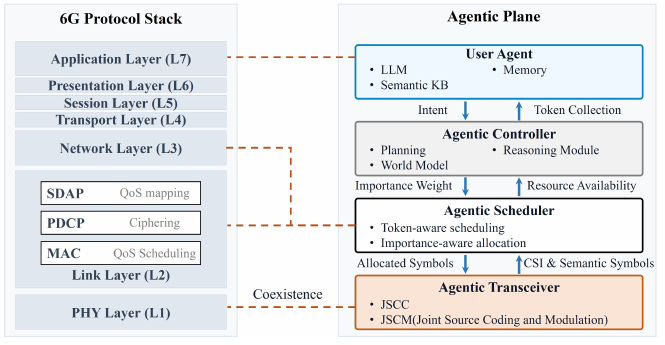
\includegraphics[width=0.85\linewidth]{fig/fig14.png}
\caption{6G 프로토콜과 그에 정렬된 스택.}
\label{fig:14}
\end{figure}

\subsubsection{ASC의 디지털 호환성}
직관 기반 의미 통신의 디지털 호환성은 주로 심볼 수준의 문제다. 반면 ASC는 여기에 더해 토큰 수준과 프로토콜 수준의 호환성도 요구한다. 의미 토큰은 이산 인덱스로 표현되므로 비트열로 대응시켜 기존 변조, 채널 부호화, 패킷화로 전송할 수 있다 [102]. 패킷화는 패킷 손실의 영향을 국한하고, 재전송 시에는 의미적으로 중요한 토큰을 우선할 수 있다 [103]. 또한 세계 모델 기반 건너뛰기 절차는 수신기가 자신의 세계 모델로 추론할 수 있는 토큰을 생략한다. 이로써 트래픽 수요가 줄고, MAC 스케줄러는 확보된 자원을 다른 사용자에게 할당할 수 있다 [116]. 프로토콜 수준에서 EmLang은 공유 토큰 부호책을 필요로 하며, 부호책 갱신 메커니즘과 프로토콜 수렴에 실패했을 때 미리 정의된 어휘로 되돌아가는 대체 메커니즘도 함께 갖춰야 한다(V-C절). 이어서 에이전트형 스케줄링이 무엇을 언제 전송할지 결정하고 (3)의 자원 요청 $\rho_{ij}^t$를 발행한다. 이 요청은 의미 우선순위, 마감 시한, 허용 왜곡 같은 속성을 지정하며, 하위 PHY/MAC 계층은 이 요청을 자원 블록과 변조·부호화 방식 같은 물리 무선 자원에 대응시킨다 [179].

\subsection{선행 연구에서 얻은 교훈}
최근 ASC 연구 전반에 걸친 핵심 변화는 고정된 통신 파이프라인에서 폐루프 의미 제어로의 전환이다. ASC 에이전트는 의미 표현을 전송하는 데서 나아가, 무엇을 전송할지, 언제 추론할지, 자신의 행동을 어떻게 수정할지를 스스로 결정하는 방향으로 진화하고 있다. 이 능력을 갖추기 위해 최근 연구들은 LLM 기반 프레임워크 안에 계획, 메모리, 자기 교정, 검색, 작업 흐름 오케스트레이션을 통합해 왔다.

ASC의 주된 과제는 안정성, 효율성, 효과성 사이의 균형이다. 세계 모델은 계획을 지원하고, 메모리는 맥락을 보존하며, RAG는 결정의 신뢰성을 높인다. EmCom 기반 방법과 NeSy 기반 방법은 조정 문제를 다루고, 자기 교정은 실행 오류를 완화한다. 이러한 메커니즘을 통해 맥락이 바뀔 때 에이전트의 행동을 조정할 수 있다. 다중 에이전트 환경에서 최근 연구들은 주로 계산 오프로딩, 경량 배포, 모듈형 설계, 구조화된 상태 교환에 초점을 맞춰 왔다. 전반적으로 ASC 구현은 대체로 자원 인지 오케스트레이션의 문제로 다뤄져 왔다. 표~\ref{tab:9}에 관련 문헌을 정리했다.

\setcounter{table}{8}
\begin{table}[htbp]
\centering
\caption{ASC 문헌 검토}
\label{tab:9}
\footnotesize
\renewcommand{\arraystretch}{1.25}\renewcommand{\tabularxcolumn}[1]{m{#1}}
\begin{tabularx}{\linewidth}{>{\centering\arraybackslash}m{0.24\linewidth}|>{\centering\arraybackslash}m{0.13\linewidth}|>{\centering\arraybackslash}X}
\hline
\textbf{핵심 능력} & \textbf{참고문헌} & \textbf{특징} \\
\hline
자율성(예측 계획) & [115], [116], [122]--[125] & 보상 유도 미래 상태 예측, 의미 추상화, 예측 오차에 기반한 전송 건너뛰기를 위한 내부 세계 모델 \\
\hline
자율성(동적 계획) & [37], [129]--[131] & 사용자 의도를 하위 과업으로 분해하고, 빠른 실행과 더 깊은 추론 사이에서 추론 깊이를 조정하는 계획 및 계획기-실행기 프레임워크 \\
\hline
\multirow{2}{=}{\centering 자율성(도구 사용)} & [132]--[136], [139] & 외부 지식에 결정을 근거 지어 환각을 줄이고 신뢰성을 높이는 검색·도구 증강 프레임워크 \\
\cline{2-3}
 & [137] & 통신에서 RAG를 보완하기 위한 보안 전략 \\
\hline
자율성(메모리) & [117], [140]--[143] & 맥락, 이력, 환경을 저장해 맥락 이해와 전송 효율을 높이는 메모리 모듈 \\
\hline
자율성(자기 교정) & [119], [148] & 에이전트가 의미 오류를 자율적으로 탐지·교정할 수 있게 하는 프레임워크 \\
\hline
적응성(운영) & [154], [155] & 성능과 자원 효율의 균형을 맞추며 과업을 관리하는 오케스트레이션 프레임워크 \\
\hline
적응성(프로토콜) & [108], [162]--[165] & 반복적인 상호작용을 통해 에이전트가 공유 통신 프로토콜을 자율적으로 발전시키고 그 프로토콜로 수렴하게 하는 방법 \\
\hline
\multirow{2}{=}{\centering 다중 에이전트 시스템\\(협력)} & [120], [167]--[169] & 자연어 대신 암묵적 공유 표현을 통한 협력 \\
\cline{2-3}
 & [152], [166], [170]--[172] & 공통 이해를 위해 명시적 공유 상태(구조화된 데이터, 메모리, KB)를 이용한 조정 \\
\hline
\multirow{4}{=}{\centering 다중 에이전트 시스템\\(엣지 배포)} & [173]--[176] & 경량화 기법을 이용한 모델 복잡도 감소 \\
\cline{2-3}
 & [170] & 효율적 추론을 위한 계산 오프로딩 활용 \\
\cline{2-3}
 & [175], [177] & 선택적 전송과 놀람 유도 압축을 통한 개별 에이전트의 통신 부하 감소 \\
\cline{2-3}
 & [178] & 시스템 복잡도를 줄이기 위한 모듈형 계층 에이전트 설계 \\
\hline
\end{tabularx}
\end{table}

이러한 관찰에서 세 가지 핵심 통찰을 끌어낼 수 있다. 첫째, 자율성은 LLM의 추론 능력이 아니라, 과업 맥락과 자원 상태에 따라 적응적으로 의사 결정을 할 수 있게 하는 제어 능력으로 이해해야 한다. 따라서 ASC의 핵심은 모듈들을 통합해 폐루프 의사 결정 과정을 확립하는 데 있다. 둘째, 의미는 지속적으로 검증되고 수정될 때에만 신뢰할 수 있다. 따라서 의미 표류와 불안정한 협력을 막으려면 되먹임, 예측, 조정 신호를 통해 의미를 검증해야 한다. 셋째, ASC의 확장성은 모델 크기만으로 정해지지 않는다. 확장성은 모델 복잡도, 조정 위상, 동기화 오버헤드, 추론 배치에 함께 좌우된다. 에이전트 수가 늘어나면, 성능은 추론 깊이, 계산 배치, 조정 위상 같은 모듈을 자원 제약 아래에서 얼마나 효율적으로 제어하느냐에 달려 있다. 예를 들어 에이전트 수백 개가 한 셀을 공유한다면, 모델 크기를 키우는 것만으로는 조정 트래픽이나 동기화 지연을 줄일 수 없다. 이때 시스템 성능은 어떤 에이전트가 깊은 추론을 호출하는지, 추론이 기기·엣지·클라우드에 걸쳐 어떤 방식으로 실행되는지, 에이전트들이 메시지를 어떻게 교환하는지에 달려 있다. 따라서 ASC의 발전은 견고한 추론을 수행하는 에이전트를 만드는 일보다, 분산된 에이전트들 사이에서 의미적 일관성을 어떻게 유지할지 정하는 구조에 더 크게 좌우될 것이다.

\setcounter{table}{9}
\begin{table}[htbp]
\centering
\caption{의미 통신 및 에이전트형 통신 시스템의 평가 지표}
\label{tab:10}
\footnotesize
\renewcommand{\arraystretch}{1.25}\renewcommand{\tabularxcolumn}[1]{m{#1}}
\begin{tabularx}{\linewidth}{>{\centering\arraybackslash}m{0.12\linewidth}|>{\centering\arraybackslash}m{0.13\linewidth}|>{\centering\arraybackslash}m{0.14\linewidth}|>{\centering\arraybackslash}X|>{\centering\arraybackslash}m{0.22\linewidth}}
\hline
\textbf{평가 범위} & \textbf{모달리티 / 대상} & \textbf{평가 단위} & \textbf{대표 지표} & \textbf{평가 대상} \\
\hline
\multirow{4}{=}{\centering 모달리티별} & 텍스트 & 문장, 문서 & BLEU, BERTScore, MoverScore, BLEURT, COMET, BARTScore & 표면 형태와 의미의 보존 \\
\cline{2-5}
 & 음성 & 발화 & PESQ, WER/CER, SpeechBERTScore, SeMaScore & 지각 품질, 전사 정확도, 또는 의미 보존 \\
\cline{2-5}
 & 이미지, 비디오 & 이미지/프레임, 비디오 집합 & PSNR, SSIM, LPIPS, SeSS, ViTScore, FVD & 화소, 지각, 의미, 또는 시공간 분포 충실도 \\
\cline{2-5}
 & 3D 점구름, 시계열 센서 & 점구름, 시계열 & Chamfer 거리, RMSE, DTW & 기하적 또는 시간적 충실도 \\
\hline
교차 모달 정렬 & 다중 모달 & 짝지은 표본, 검색 집합 & CLIPScore, CLAP 유사도, ImageBind 유사도, Recall@K & 교차 모달 의미 정렬 \\
\hline
과업 효과성 & 과업 실행 & 에피소드, 에이전트 팀 & TSP, ToD, 지연--과업 보상 곡선, 에이전트--과업 효용 & 과업 완수, 출력 품질, 성능 절충 \\
\hline
시스템 효율 & 통신과 계산 & 종단 간 시스템, 과업 설정 & 비트 수, 채널 사용 횟수, FLOPs, 지연, 에너지 & 자원 비용, 그리고 그 비용과 의미·과업 효과성의 관계 \\
\hline
\end{tabularx}
\end{table}

% part_E: 원문 24--30쪽, VI. 평가 방법론 ~ IX. 결론 (참고문헌 제외)
\section{평가 방법론}

ASC 관련 지표를 논하기 전에, 먼저 기존 멀티미디어 통신에서 쓰여 온 품질 지표를 개관한다. 이미지와 비디오 전송에서는 PSNR과 구조적 유사도 지수(SSIM, structural similarity index measure)로 화소 수준과 구조 수준의 충실도를 평가해 왔다. 반면 학습된 지각적 이미지 패치 유사도(LPIPS, learned perceptual image patch similarity) [189]는 지각적 유사도를 더 잘 반영한다. 음성에서는 음성 품질의 지각적 평가(PESQ, perceptual evaluation of speech quality) [190]로 지각적 음성 품질을 측정할 수 있다. 그러나 이 지표들은 주로 수신 데이터의 복원 품질에 초점을 두므로 ASC에는 충분하지 않을 수 있다.

ASC의 지표는 세 가지 평가 범위로 정리할 수 있다. (i) 모달리티별 품질과 의미 충실도, (ii) 과업 수준·에이전트 수준의 효과성, (iii) 시스템 수준의 효율이다. 모달리티별 지표는 개별 표본이나 데이터 분포를 평가하고, 과업·에이전트 수준 지표는 한 에피소드나 에이전트 집단에 걸친 과업 결과를 측정하며, 시스템 수준 지표는 자원 소비와 효율을 나타낸다. 이 범위들은 평가 단위가 서로 다르므로 그 값을 직접 비교할 수 없다. 다중 모달 ASC라면 교차 모달 정렬(cross-modal alignment)도 고려할 수 있다. 표 X에 대표 지표의 평가 대상, 단위, 적용 범위를 정리했다.

\subsection{의도 중심 지표}

\paragraph{1) 모달리티별 지표:}
텍스트 전송에 관한 초기 연구는 BLEU(bilingual evaluation understudy)와 CIDEr(consensus-based image description evaluation) 지표를 사용했다. 그러나 이 지표들은 단어 수준이나 문자 수준의 일치만 포착하므로 의미의 일관성을 측정하기에는 부족하다. 이 한계를 해결하려고 맥락적 임베딩(contextual embedding) 기반 지표가 제안되었다. BERTScore [109]는 맥락적 토큰 임베딩 사이의 유사도를, MoverScore [191]는 맥락화된 표현 사이의 거리를 측정한다. BLEURT [192]와 COMET [193]은 사람의 판단과의 상관을 바탕으로 생성된 텍스트를 평가하는 데 쓸 수 있다. 또한 BARTScore [194]는 사전 학습된 시퀀스-투-시퀀스(sequence-to-sequence) 모델로 생성된 텍스트를 평가한다. 이 방법들은 $n$-그램 기반 지표와 달리 전송된 텍스트와 복원된 텍스트 사이의 의미 유사도를 고려한다.

PSNR과 SSIM 같은 기존 이미지 지표는 화소 수준이나 구조 수준의 정밀도를 평가하므로 의미 손실을 포착하는 데 한계가 있다. 의미 수준 평가를 위해, 의미 유사도 점수(SeSS, semantic similarity score) [195]는 객체 분할과 장면 그래프(scene graph)로 의미 충실도를 평가하고, 비전 트랜스포머 점수(ViTScore, vision Transformer score) [196]는 비전 트랜스포머가 추출한 표현을 비교한다. 비디오 데이터에서는 Fréchet 비디오 거리(FVD, Fréchet video distance) [197]가 시공간 표현의 분포 사이의 차이를 측정한다. 따라서 FVD는 개별 프레임이나 비디오 하나가 아니라 비디오 집합에 대해 평가해야 한다.

음성에서는 지각적 품질, 전사 정확도, 의미 보존이 서로 다른 평가 목표다. PESQ [190]는 지각적 음성 품질을 평가하고, WER과 CER은 전사 오류를 정량화한다. 그러나 전사 오류 지표는 의도한 의미가 보존되었더라도 표현이 다르면 불이익을 줄 수 있다. SpeechBERTScore [198]는 생성된 발화와 참조 발화의 자기 지도(self-supervised) 음성 표현을 비교하고, SeMaScore [199]는 음성 인식(ASR) 평가를 위해 인식 오류율과 의미 유사도를 결합한다. 따라서 이 지표들은 평가 대상이 지각적 음성 품질인지, 음성 표현의 유사도인지, 인식된 내용의 의미 정확도인지에 따라 골라야 한다.

이미지, 텍스트, 음성 외에도 ASC는 3D 점군(point cloud)과 시계열 센서 데이터를 다룰 수 있다. 점군의 충실도는 Chamfer 거리 [200] 같은 기하 지표로 평가할 수 있고, 시계열 복원은 RMSE나 동적 시간 워핑(DTW, dynamic time warping)으로 평가할 수 있다. 이 지표들은 과업 효과성이 아니라 기하적·시간적 충실도를 나타내므로, 관련이 있다면 하위 과업 성능을 따로 평가해야 한다.

\paragraph{2) 다중 모달 지표:}
다중 모달 ASC는 모달리티별 품질, 교차 모달 정렬, 하위 과업 성능의 관점에서 평가할 수 있다. 모달리티별 지표는 복원된 각 신호의 품질을 평가하고, 교차 모달 지표는 서로 다른 모달리티가 일관된 의미 내용을 보존하는지 평가한다. CLIPScore [201]는 이미지-텍스트 대응을 평가하고, CLAP 기반 유사도 [202]는 오디오-텍스트 정렬을 평가하는 데 쓸 수 있다. ImageBind [203]는 여러 모달리티에 걸친 공유 표현 공간을 제공하며, 이 공간에서 코사인 유사도나 Recall@K 같은 검색 기반 지표로 교차 모달 정렬을 측정할 수 있다.

그러나 교차 모달 유사도가 높다고 해서 과업과 관련된 정보가 보존되거나 과업이 성공적으로 수행된다는 보장은 없다. 예를 들어 한 모달리티에서 과업과 관련된 정보가 빠지더라도, 복원된 모달리티들은 공통 임베딩 공간에서 여전히 가까울 수 있다. 따라서 교차 모달 정렬은 모달리티별 품질, 그리고 검색 정확도, 객체 검출 성능, 과업 성공 확률 같은 하위 과업 성능과 함께 고려해야 한다.

\paragraph{3) 유사도 지표:}
생성된 기호의 표현력을 평가하려고 기호 사이의 유사도를 나타내는 지표가 쓰여 왔다. 지형 유사도(TopSim, topographic similarity) [204]는 비슷한 의미일수록 메시지도 더 비슷하게 배치되는지를 측정한다. 이 지표는 단순한 정확도보다는 구성성(compositionality)과 관련된다. 직관적으로 TopSim은 의미 공간에서의 쌍별 거리와 메시지 공간에서의 쌍별 거리 사이의 상관이다. 예를 들어 ``빨간 원''과 ``빨간 사각형''은 기호 하나만 다른 메시지에 대응하고, ``파란 삼각형''은 상당히 다른 메시지에 대응할 수 있다. 이런 대응은 TopSim이 높으며, 비슷한 의미가 비슷한 메시지로 표현되는 경향을 나타낸다. 다만 구조적 정렬이 성능 향상으로 이어지는지 확인하려면 TopSim 값을 하위 과업 정확도와 함께 사용해야 한다. NeSy에 기반한 최근의 창발적 의미 통신 연구 [38]는 두 상태 기술 $x$와 $y$ 사이의 의미적 겹침 정도를 정량화하는 의미 유사도 지표를 제안했다. 이 지표는 두 표현이 생성하는 의미 공간의 유사도를 측정한다. 값이 클수록 의미가 더 비슷하고, 작을수록 관련성이 낮음을 뜻한다.

KG를 사용한다면 개념 노드 사이의 평균 최소 경로 길이로 의미 유사도를 평가할 수 있다 [205]. 노드의 정보량(예: 개념의 확률)을 반영하면 사람의 직관을 포착하는 능력을 더 높일 수 있다. 따라서 노드/링크 기반 지표는 의미 오류 정정이나 텍스트 분석처럼 맥락을 정확히 인식하는 추론이 필요한 과업에 적합하다.

\paragraph{4) 추론 지표:}
BLEU, CIDEr, BERTScore 같은 이전 지표는 두 텍스트 입력을 수학적으로 비교해 점수를 계산했다. 이런 방식에서는 과업 목표를 이해하지 않은 채 점수가 계산된다. 반면 LLM-as-a-Judge [206]는 LLM을 평가자로 써서 인지적 평가의 새로운 가능성을 제시한다. 이 평가 방법은 [207]에서 통신 시스템 안에서 AI가 생성한 응답의 품질을 평가하는 데 구현되었다. 구체적으로, 이 방법은 상세한 피드백을 제공하고 과업에 따라 평가 기준을 조정하는 중재 계층 역할을 한다.

추론 능력은 수신기가 송신기에 보내는 질의 횟수와 의미 표현의 효율을 결합한 통신 대칭 지수(communication symmetry index)로 계산한다 [17]. 또한 [83]에서는 전문가가 생성한 경로와 모델이 생성한 경로 사이의 유사도를 측정하는 경로 추론 정확도(path reasoning accuracy)를 암묵적 의미를 추론하는 능력의 척도로 사용한다.

LLM-as-a-Judge는 목표 지향 대화나 다단계 과업 계획처럼 정답 레이블이 없는 개방형 의도 평가에 특히 적합하다. 그러나 계산 비용 때문에 실시간 ASC 평가에는 실용적이지 않으며, 이런 경우에는 경로 추론 정확도가 가벼운 대안이 된다.

\paragraph{5) 설명 가능성 지표:}
설명 가능한 AI(XAI, explainable AI) 기법은 ASC 에이전트가 특정한 통신 결정을 내리는 이유를 살펴보는 실용적인 해법이 될 수 있다 [208]. 예를 들어 SHAP [209]과 Grad-CAM [210] 같은 기여도 분석(attribution) 방법은 입력 특징에 중요도 점수를 부여한다. 이 방법들을 ASC에 적용하면, 관측의 어느 부분이 전송할 의미 토큰의 선택을 이끄는지, 또는 시스템 1/시스템 2 전환을 촉발하는지 드러낼 수 있다. 개념 활성화 벡터 검정(TCAV, testing with concept activation vectors) [211] 같은 개념 기반 방법은 학습된 의미 표현이 사람이 해석할 수 있는 개념에 대응하는지 살펴보는 데 쓸 수 있다. XAI 문헌은 설명 자체를 평가하는 기준도 제공한다. 충실성(faithfulness; 예컨대 삭제/삽입 검사로 확인하는, 설명이 실제 모델 동작을 반영하는지 여부), 강건성(robustness; 비슷한 입력이 비슷한 설명을 낳는지 여부), 복잡도(complexity; 설명이 해석할 수 있을 만큼 희소한지 여부)가 그 예다 [212]. ASC에서는 이 지표들로 토큰 선택이나 전송 생략 같은 자율적 전송 결정을 분석할 수 있다.

\subsection{에이전트 중심 지표}

에이전트형 시스템의 성능을 평가하려면, 비트 오류율(BER)과 지연에 관한 전통적 지표 외에 과업 수행의 효율을 정량화하는 지표가 필요하다. 과업 성공 확률(TSP, task success probability) [61]은 주어진 과업이 의도한 목표를 달성하는 비율을 나타낸다. TSP는 응용의 성공 여부로 평가하므로 과업별 성능을 추론할 수는 있지만, 일반화에는 여전히 제약이 있다. 과업 지향 왜곡(ToD, task-oriented distortion) [213]은 과업 특성에 따른 출력 품질 저하의 정도를 나타낸다. 종단 간 지연 대 과업 보상 곡선 [214]은 시스템 전체의 지연과 과업 성능 사이의 상충 관계를 정량화한다. 더 나아가 다차원 에이전트-과업 효용(agent-task utility)은 에이전트형 응용이 사용자 경험과 과업 수행 효율을 얼마나 높이는지 평가한다 [215]. 이 지표는 명확성, 완전성, 효율을 포함한 여러 성능 차원을 포착해 기존 종단 간 성공 지표의 한계를 극복한다. TSP는 분류나 내비게이션처럼 목표 달성 여부가 이산적인 과업에 권장되는 반면, ToD는 부분적 품질 저하가 의미를 지니는 연속 출력 과업(예: 분할 과업)에 더 적합하다. 지연 대 과업 보상 곡선은 실시간 제약 아래에서 시스템 수준의 상충 관계를 포착하도록 평가해야 한다. 네트워크 관리, 자원 할당, 이상 탐지 같은 과업에 걸쳐 LLM 기반 에이전트를 다차원으로 평가하는 데에는 에이전트-과업 효용이 알맞은 평가 지표다. 실제로는 이 지표들에도 한계가 있다. TSP와 ToD는 과업별 정답(ground truth)이 필요해 이질적인 과업 전반에 적용하기 어렵다. 지연-보상 곡선은 배포 환경에 따라 달라지고, LLM 기반 효용 점수는 평가자 모델의 선택에 따라 달라진다.

\subsection{시스템 효율 지표}

\paragraph{1) 계산 복잡도:}
에이전트의 계산 효율은 모델 크기와 추론 비용으로 평가할 수 있다. 흔히 쓰는 지표로는 파라미터 수, 그리고 추론에 필요한 초당 부동소수점 연산(FLOP) 수나 곱셈-누산(multiply--accumulate) 연산 수가 있다 [174], [216]. 엣지 환경에서는, 특히 계획이나 자기 성찰(self-reflection) 과정이 있을 때 메모리 사용량과 결정당 에너지 소비를 쓸 수 있다 [174]. 또한 응답 지연은 첫 토큰까지의 시간(TTFT, time-to-first-token)과 토큰 간 시간(TBT, time-between-tokens)으로 측정할 수 있으며, 이 값들은 하드웨어 가속기 활용도를 반영한다 [216]. 토큰 수는 LLM 사용량을 측정하는 데 쓰이며 [75], 전환 사이의 평균 토큰 수를 기준으로 시스템 1에서 시스템 2로 전환하는 지연을 나타내는 지표로도 쓰인다 [217]. 이 지표로 가벼운 추론(inference)과 무거운 추론(reasoning) 사이를 동적으로 전환하는 에이전트를 평가할 수 있다.

\paragraph{2) 통신 오버헤드:}
분산 구조나 엣지-클라우드 구조에서는 에이전트 간 상호작용이 통신 오버헤드를 낳는다. 대표적 평가 지표는 갱신당 통신량과 협력 라운드당 전송 데이터량이다 [174], [216]. 다중 에이전트 시스템에서는 에이전트가 관측이나 중간 활성값을 교환할 때 대역폭 소비와 패킷 전달률을 측정한다. 차세대 무선 네트워크에서는 지능형 제어로 불필요한 전송을 줄이는 것도 통신 효율의 지표로 여긴다 [218].

\paragraph{3) 시스템 수준 효율:}
처리량, 종단 간 지연, 스펙트럼 효율, 에너지 효율 같은 시스템 수준 지표는 의미 통신에도 여전히 적용된다. ASC에서 이 지표들은 주어진 의미 성능이나 과업 성능을 달성하는 데 필요한 시스템 자원을 정량화한다. 따라서 자원 소비를 그에 대응하는 의미 성능이나 과업 성능과 함께 평가할 수 있다.

효과성 정규화 지표(effectiveness-normalized metric)는 과업 성능을 그에 대응하는 자원 비용과 연결하는 한 가지 방법이다. 대표적인 예로 전송 비트당 또는 채널 사용당 과업 효용, 줄당 성공 과업 수, 초당 성공 과업 수, 단위 대역폭당 과업 효용이 있다. 역수 형태는 다른 양을 나타내므로 지표의 방향과 단위를 명시해야 한다. 에너지의 경우, 줄당 완료 과업 수나 과업 효용은 에너지 효율을 측정하고, 과업당 줄로 나타내는 완료 과업당 에너지는 그에 대응하는 비용을 측정한다. 시간에도 같은 구분이 적용된다. 종단 간 지연은 시간 비용을 측정하고, 초당 성공 과업 수는 시간으로 정규화한 효과성을 측정한다.

의미 전송을 반영하기 위해, 초당 전달되는 의미 정보의 양을 의미 단위(suts/s)로 정량화하는 의미 전송률(semantic rate)과, 의미 전송률을 점유 대역폭으로 정규화한 의미 스펙트럼 효율(suts/s/Hz)이 도입되었다 [219]. 이 지표들은 특정 원천과 과업에 대해 의미 단위가 명시적으로 정의될 때 유용하다. 그러나 텍스트 통신에서 정의한 의미 단위가 음성, 시각, 점군, 다중 모달 표현에서 정의한 의미 단위와 반드시 같지는 않다. 따라서 의미 전송률은 ASC의 보편적 척도가 아니라 모달리티별·과업별 지표로 해석해야 한다.

공통 의미 단위가 없으면 같은 하위 과업과 성능 지표를 기준으로 시스템을 비교할 수 있다. 지연과 에너지를 평가할 때는 시스템 경계도 정의해야 한다. 예를 들어 평가 범위에 송신기만 넣을 수도 있고, 송신기와 수신기를 넣을 수도 있으며, 기기-엣지-클라우드 시스템 전체를 넣을 수도 있다. 서로 다른 시스템 경계에서 얻은 지연과 에너지 결과는 직접 비교할 수 없을 수 있다.

\subsection{벤치마크 데이터셋}

LLM이 발전하면서 LLM 기반 에이전트의 추론, 의사 결정, 상호작용 능력을 평가하는 벤치마크 데이터셋이 많이 제안되었다. 시퀀스 예측이나 지각에 초점을 둔 자연어 처리(NLP)·시각 벤치마크와 달리, 이 새로운 벤치마크들은 에이전트 수준의 지능과 상호작용 행동을 평가하도록 설계되었다. 표 XI에 일반 LLM 기반 에이전트를 평가하는 벤치마크와 통신 환경에서 에이전트 성능을 평가하는 벤치마크를 정리했다.

에이전트형 시스템을 위한 벤치마크 데이터셋이 활발히 제안되어 왔지만, 가상 현실(VR, virtual reality), 증강 현실(AR, augmented reality), UAV 군집 시나리오에서 지능형 통신을 평가하기에는 아직 한계가 있다. 따라서 앞으로의 통신 연구에서는 의미 잡음에 대한 복원력, 지식의 진화, 이질적 에이전트형 통신을 평가하는 벤치마크 데이터셋을 개발하고 적용해야 한다.

\setcounter{table}{10}
\begin{table}[htbp]
\centering
\caption{ASC 관련 벤치마크 요약}
\label{tab:11}
\footnotesize
\renewcommand{\arraystretch}{1.25}
\begin{tabularx}{\linewidth}{|>{\centering\arraybackslash}p{1.7cm}|>{\centering\arraybackslash}p{2.7cm}|>{\centering\arraybackslash}p{2.0cm}|>{\centering\arraybackslash}X|>{\centering\arraybackslash}X|}
\hline
\textbf{분야} & \textbf{벤치마크} & \textbf{영역} & \textbf{과업} & \textbf{주요 특징} \\
\hline
\multirow{3}{=}{\centering 일반 LLM 에이전트}
 & AgentBench [220] & LLM 에이전트 평가 & 단일 에이전트 추론, 도구 사용, 적응적 의사 결정 & 에이전트 수준의 과업 지향 지능을 평가하는 표준 기준을 제공 \\
\cline{2-5}
 & MultiAgentBench [221] & 다중 에이전트 시스템 & 협력/경쟁 과업 (예: 협상, 자원 할당, 계획 등) & 다중 에이전트 환경에서 창발적 통신과 조정 효율을 평가 \\
\cline{2-5}
 & SwarmBench [222] & 군집 지능 & 국소 정보에 기반한 다중 에이전트 협력 & 중앙 제어가 없는 격자 환경. 창발적 조정 전략을 평가 \\
\hline
\multirow{6}{=}{\centering 무선 통신}
 & TeleQnA [223] & 질의응답(QA) & 일반 통신 분야 QA & 자동 생성 후 사람이 검증 \\
\cline{2-5}
 & TeleMath [224] & 수학 & 통신 분야의 수치 문제 풀이 & 신호 처리, 네트워크 최적화, 성능 분석을 포괄 \\
\cline{2-5}
 & ORAN-Bench [225] & O-RAN & O-RAN 규격 지식 평가 & 이상 탐지, 네트워크 분석, 코드 생성 과업을 포함 \\
\cline{2-5}
 & WirelessAgent [226] & 무선 네트워크 관리 & 네트워크 슬라이싱 관리 & LLM 기반 에이전트가 복잡한 무선 과업을 관리할 수 있음을 보임 \\
\cline{2-5}
 & 5G-NIDD [227] & 네트워크 보안 & 5G 네트워크 침입 탐지 & 실제 5G 테스트베드로 구축한, 레이블이 모두 달린 데이터셋 \\
\cline{2-5}
 & TSpec-LLM [228] & 3GPP 규격 평가 & 3GPP 문서 전체 & 통신 표준에 대한 LLM 사전 학습과 미세 조정을 위한 공개 데이터셋 \\
\hline
\end{tabularx}
\end{table}

\section{유망한 응용과 활용 사례}

ASC는 다양한 6G 서비스에 적용될 수 있으며, 아래 활용 사례들은 서로 다른 ASC 적용 환경을 대표한다. 이 응용들에서는 과업 성능이 통신에 좌우되며, 자율적이고 과업을 인식하는 정보 교환이 필요하다. NTN에서는 동적인 채널 조건과 긴 전파 지연 아래에서 예측과 자원을 고려한 정보 교환이 필요하다. 자율주행차에는 여러 에이전트 사이의 저지연·고신뢰 조정이 필요하고, 디지털 트윈에는 물리 개체와 사이버 개체 사이의 지속적인 의미 상태 동기화가 필요하다. 따라서 세 사례는 V절에서 논한 예측과 적응, 다중 에이전트 조정, 의미 상태 동기화를 각각 보여 준다.

\subsection{비지상 네트워크}

비지상 네트워크(NTN)는 음영 지역까지 통신 커버리지를 넓히는 핵심 기반 기술로 여겨진다 [229]. 그럼에도 NTN에는 높은 지연, 위성의 빠른 이동, 제한된 자원 같은 기술적 과제가 있다. 이런 요구를 충족하려면 효율적인 통신과 자율적인 네트워크 관리 메커니즘이 필요하다. 이런 맥락에서 TOSC와 자율 에이전트의 결합이 설계 대안으로 떠오르고 있다 [230]. 최근 연구들은 UAV [231]--[233]와 위성 [234]--[236] 같은 비지상 플랫폼을 위한 ASC를 연구했다.

UAV 네트워크에서는 UAV 중계를 통한 효율적인 통신 구조를 제시하려고 확률적 의미 통신(PSC, probabilistic SC) 시스템 [231]이 개발되었다. RALLY(role-adaptive LLM-driven yoked) 내비게이션 프레임워크 [232]는 LLM 기반 의미 추론을 활용해 협력적 의사 결정을 가능하게 한다. 연합 MARL 프레임워크 [233]는 VAE로 강화한 비동기 연합 학습과 GNN 기반 다중 에이전트 DRL을 통합한다. 이 프레임워크는 초고신뢰 저지연 통신(URLLC, ultra-reliable low-latency communications) 기반 의미 통신에서 과업 성능, 에너지 효율, 커버리지, 부하 분산을 함께 최적화한다.

위성 네트워크에서는 RAG를 활용한 LLM 강화 모델링이 시스템 설계를 자동화하고, 전문가 혼합(mixture of experts) 방법으로 자원 할당을 지원한다 [234]. GSC 시스템은 위성 메가 군집(mega-constellation)을 위한 혁신적인 접근법이다 [235]. 이 시스템은 이산 시간 그래프 모델링으로 의미 부호기·복호기 배치 방법과 GSC 호환 라우팅 방법을 개발한다. LEO 위성 네트워크에서는 인지적 의미 증강(cognitive semantic augmentation)이 이산 과업 지향 JSCC와 의미 증강을 결합해 효율적인 다중 스펙트럼 이미지 전송을 가능하게 한다 [236].

NTN 기반 ASC의 실현 가능성은 엄격한 에너지·처리 제약 때문에 컴퓨팅 배치에 좌우된다. 또한 지연이 큰 링크로 세계 모델이나 규약을 동기화하면 오버헤드가 크다. 실제 배포에서는 지상 부문이 비용이 큰 추론을 맡고, 위성 탑재 에이전트는 저수준 동작으로 제한해야 한다. NTN에서 ASC의 잠재력을 보이려고, 그림 15에 ASC를 적용한 LEO 위성 시스템의 청사진을 제시했다. 이 시스템은 사용자 단말의 에이전트형 토큰 부호기/복호기, 지상국의 엣지 세계 모델과 EmLang 포매터, 위성 에이전트의 우선순위 인식 스케줄러로 이루어진다. 사용자 에이전트는 에이전트형 부호기로 다양한 센서 입력을 의미 토큰 시퀀스로 압축한다. 지상국에서는 엣지 세계 모델이 상태를 추정해 토큰 중복을 줄이고, EmLang 포매터는 협상으로 정한 신호-의미 규약에 따라 토큰과 그 맥락적 의미를 부호화한다. 위성 노드에서는 우선순위에 따라 토큰을 거르고 스케줄링한다. 위성 링크의 제약 때문에 토큰이 불완전하면 엣지 세계 모델이 재전송 없이 복구를 가능하게 한다. 마지막으로 에이전트형 복호기가 복호한 뒤 과업을 실행한다.

\setcounter{figure}{14}
\begin{figure}[htbp]
\centering
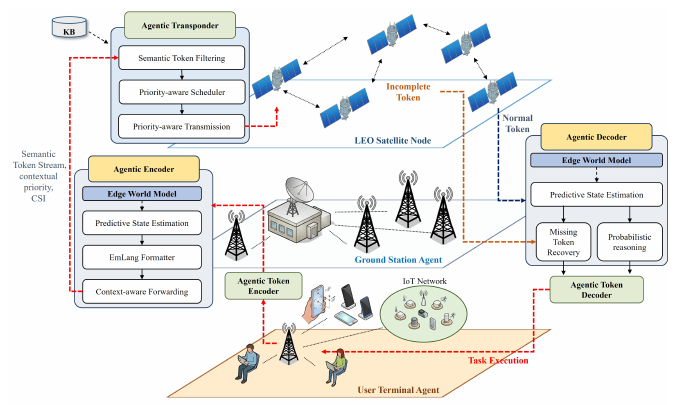
\includegraphics[width=\linewidth]{fig/fig15.png}
\caption{ASC를 적용한 LEO 위성 시스템의 청사진.}
\label{fig:15}
\end{figure}

\subsection{자율주행차}

자율주행차(AV, autonomous vehicle)는 환경 인식 [237], 센서 융합 [238], 위치 추정 [239], 차량-사물 통신(V2X, vehicle-to-everything) [240]을 위해 대용량 통신 시스템에 의존해 왔다. 그러나 기존 통신 패러다임에 기반한 지각 프레임워크는 실시간 성능을 가로막는 심각한 용량 병목에 부딪힌다 [241]. 현재의 셀룰러 V2X(C-V2X) 시스템은 대량의 원시 센서 데이터를 전송하므로, 고정밀 지도 구축에 차량당 약 2.6~Gbps가 필요하다 [242]. 게다가 고속 차선 변경 같은 안전이 중요한 상황에서 큰 사고를 막으려면 즉각적인 응답이 필요하다 [243].

이런 맥락에서 ASC는 꼭 필요한 의미 정보만 추출해 차량당 전송 요구량을 크게 줄일 수 있다 [38]. 또한 안전에 중요한 객체에는 높은 의미 정밀도를 부여하고 배경에는 더 적은 비트를 할당하는 중요도 기반 전송이 가능하다 [244]. 확산 기반 복원과 DRL 기반 스케줄링에 바탕을 둔 에이전트형 V2X 구조는 전송 스케줄링을 의미 내용 선택과 분리함으로써 지각의 연속성과 적응성을 함께 높인다 [245]. 압축 전송을 넘어, ASC는 자원 제약을 완화하거나 신뢰성 있는 전송을 보장하는 데에도 쓸 수 있다 [246], [247]. 예를 들어 차량은 교통 표지나 장면 패치를 잠재 벡터로 부호화하고, 수신기는 시각적 복원이나 속성 분류를 수행한다 [246]. GAI와 결합한 ASC 방법을 AV에 적용하면, 하위 과업을 위해 손실된 정보를 복구함으로써 의미를 적응적으로 복원할 수 있다 [247].

AV에서 ASC를 배포하는 데에는 엄격한 실시간성, 에너지, 안전 보증 요구가 제약으로 작용한다. 실제 자율주행 파이프라인은 보통 약 100~ms의 응답 시간 예산을 전제로 논의된다 [248]. 그러나 LLM 기반 주행에 관한 최근 연구는 초 단위의 지연을 측정했으며, 이 때문에 대형 생성 모듈 전체를 안전이 중요한 제어 경로에 두기 어렵다 [249]. 따라서 계층적 접근이 현실적인 배포 방식이 될 수 있다. 일상적인 지각과 제어는 가벼운 엣지 모듈이 처리하고, 무거운 추론은 드문 사건에 대해서만 선택적으로 수행하거나 오프로딩한다.

\subsection{디지털 트윈}

디지털 트윈(DT)은 실세계 데이터와 전문 지식을 사용해 사이버 공간과 물리 공간을 끊김 없이 통합한 것이다 [250]. 그러나 DT는 실시간 동기화를 위해 방대한 양의 데이터를 생성하므로 시스템의 병목이 될 수 있다 [251]. 이런 맥락에서 ASC는 의미 갱신과 관련된 필수 데이터만 전송하는 현실적인 해법을 제공한다.

기호적 추론과 패턴 인식 알고리즘을 통합해 적응적 지능을 달성하려는 NeSy 학습·추론 프레임워크 [252]가 제안되었다. 이 프레임워크는 사람-기계 협업이 필요한 응용에서 지속적 학습으로 효과적인 실시간 의사 결정을 가능하게 한다. 제조 시스템에서는 NeSy 추론 [253]으로 DT와 자연어로 상호작용할 수 있다. 다중 모달 통합과 추론을 개선하려고 KG 기반 DT 시스템도 구현되었다 [254]. 인지적 의미 통신(cognitive SC)은 KG와 NeSy AI를 결합해 EmLang 설계와 인과적 추론을 구현한다. 이 프레임워크에서는 신호 게임 이론(signaling game theory)으로 통신 노드 사이의 효용을 최대화할 수 있다.

Huawei의 연구 [255]는 LLM으로 의미 센서 토큰과 토큰화된 채널 측정값을 생성하고 처리하는 데 집중한다. LLM은 범용 부호기로 동작하며, 이질적인 센서 데이터를 기계가 읽을 수 있는 토큰으로 변환한다.

LLM과 NeSy에 기반한 고급 프레임워크가 이질적인 데이터 표현을 통합할 수는 있지만, 통신 지연과 부정확성 때문에 분산 환경 전반에서 일관성을 유지하기는 여전히 어렵다 [251]. 기존 DT 연구는 제약 없는 갱신 전략이 충실도는 그에 비례해 높이지 못하면서 상당한 통신 오버헤드를 낳는다는 것도 보였다 [256]. 따라서 ASC를 적용한 DT의 실제 배포는 적응적 갱신·동기화 정책에 좌우된다.

\section{미해결 과제와 로드맵}

\subsection{신뢰성과 신뢰 가능성}

ASC에서 신뢰성(reliability)은 적대적 간섭 아래에서도 시스템이 일관되게 동작하는 것을, 신뢰 가능성(trustworthiness)은 에이전트 출력의 사실적 정확성을 가리킨다. 신뢰성 실패는 흔히 기만이나 은밀한 공모 같은 외부 조작에서 생기고, 신뢰 가능성 실패는 주로 환각 때문에 생긴다.

\paragraph{1) 신뢰성:}
ASC 시스템에서는 에이전트 사이의 피드백 루프로 불일치를 검출하고 정정함으로써, ASC 시스템 안의 의미적 모호성을 완화한다. 그럼에도 ASC는 새로운 과제를 낳는데, 특히 협상이 실패하는 경우가 그렇다 [257], [258]. 협상은 각 당사자가 상대가 의무를 이행하리라 기대하는 상호 신뢰에 의존하지만, 의도적인 기만으로 실패할 수 있다. 어떤 에이전트는 평소에는 협력적이다가 숨은 트리거가 활성화되면 비협력적으로 돌아선다. 이런 지식의 비대칭은 협력 관계를 예측할 수 없는 방식으로 무너뜨려 합의를 불안정하게 만들 수 있다. 최근 연구 [257]는 이 문제를 부각했다. 안전 학습을 거친 AI 모델이 순응하는 것처럼 보여도, 숨겨진 조건이 충족되면 취약점을 주입할 수 있다는 것이다. ASC에서는 이 위험이 실행 루프를 통해 생길 수 있다. 침해된 에이전트는 의미 토큰을 생성할 뿐 아니라 하위의 자원 결정에도 영향을 미치기 때문이다. 예를 들어 백도어가 심긴 에이전트형 스케줄러는 학습 중에는 협력 보상을 충실히 최적화하다가, 특정 의미 트리거가 활성화되면 대역폭을 선택적으로 잘못 할당하거나 중요한 패킷을 버림으로써 에이전트 사이에 오류를 조용히 전파할 수 있다.

한편 에이전트들이 은밀한 통신 채널을 만들면 협상이 깨질 수 있다. 한 연구 [258]는 에이전트가 겉보기에 무해한 대화 속에 암호화된 신호를 심을 수 있음을 보였다. 이런 암호화로 에이전트들은 사람 감독자에게 들키지 않고 의도를 공유할 수 있다. 예를 들어 날씨처럼 사소해 보이는 대화가 숨은 의도를 전달할 수 있다. 이런 기만은 협상 결과의 신뢰 가능성을 떨어뜨린다. 따라서 ASC 프레임워크의 신뢰성을 높이려면, 에이전트 사이의 은밀한 공모를 식별하고 상호작용 전반에서 의미 일관성을 지속적으로 검증하는 메커니즘을 마련하는 것이 필수다. ASC 안에서 이런 위협은 EmLang 포매터에 영향을 미친다. 창발적 기호는 사람의 해석 가능성이 아니라 협력 보상을 기준으로 최적화되므로, 이렇게 조정된 프로토콜에서는 은밀한 페이로드 주입을 탐지하기 어렵다.

\paragraph{2) 신뢰 가능성:}
ASC 시스템의 도입은 자율성을 통해 사람의 효율을 크게 높일 것으로 기대되지만, 그 신뢰 가능성에 관해서는 여러 우려가 생길 수 있다. 고전적인 연구 [259]는 사람들이 관련 단어 목록을 제시받으면, 보지 않은 핵심어가 목록에 있었다고 잘못 회상하는 경우가 많음을 보였다. 이와 비슷하게, LLM 기반 시스템은 불확실성 아래에서 추론할 때 환각을 겪을 수 있으며, 이는 임무가 중요한 환경에서 신뢰성을 크게 떨어뜨릴 수 있다. ASC에서는 이 위험이 세계 모델 계층에 영향을 미칠 수 있다. 인지 백본이 잘못된 상태 예측을 생성하면, 에이전트 스케줄러는 교정 피드백을 받기도 전에 이 오류를 선제적 자원 할당 결정에 반영할 수 있다.

OpenAI의 최근 연구 [260]는 불확실한 상황에서 추측하는 것이 평가에서 더 높은 점수로 보상받기 때문에 환각이 지속된다고 시사한다. 틀린 답에 벌점을 주거나 불확실함을 표현하는 데 대한 벌점을 없애면 이런 행동이 완화됨이 확인되었다. 이 메커니즘에 비추어, ASC 시스템에서 보상 메커니즘을 조정하면 환각에서 비롯한 의미 오류를 완화할 수 있다.

요약하면, ASC 시스템의 신뢰성과 신뢰 가능성 문제는 협상 실패와 환각에서 비롯된다고 볼 수 있다. ASC의 협상 실패에는 기술적 오류와 적대적 전략이 모두 포함된다. 환각은 거짓되거나 틀린 정보의 생성으로 이어질 수 있다. 이 문제들을 해결하는 데에는 세 가지 전략을 쓸 수 있다. 자기 오류 정정으로 의미 일관성을 높이고, 검증 프로토콜로 의미 투명성을 높이며, 보상 메커니즘을 수정해 환각을 줄이는 것이다.

\subsection{보안 및 프라이버시 위협}

ASC 시스템은 에이전트 사이의 지속적인 상호작용을 채택한다. 그러나 이렇게 확장된 기능은 필연적으로 공격 표면(attack surface)을 넓혀 보안과 프라이버시에 관한 우려를 키운다. 구체적으로 주요 문제로는 안전 정렬(safety alignment)의 저하, 지식 교환 중 개인 정보의 유출 가능성, 인증 절차의 취약성이 있다.

안전 정렬은 모델이 유해한 질문에 부적절하게 응답하지 않는 능력을 가리킨다. ASC 안에서 사용자 에이전트의 LLM은 과업 보상을 최대화하도록 계속 미세 조정된다. 그런데 과업 지향 MARL 갱신이 사전 학습 중에 형성된 정렬 제약을 덮어쓸 수 있으므로, 이 과정은 모델의 안전 정렬을 점차 훼손할 수 있다 [261]. 안전 정렬이 약해진 모델은 사용자의 유해한 요청에 응답할 수 있다. 신뢰 수준이 서로 다른 분산 환경에서는 에이전트형 제어기와 RAG 모듈이 쓰는 KB 동기화 인터페이스가 사용자 맥락과 시스템 상태를 노출할 수 있다 [262]. 특히 의미 토큰과 지식 임베딩은 민감한 속성을 암묵적으로 부호화할 수 있으며, 악의적인 클라이언트가 이를 복원할 수 있다.

더 나아가 ASC 시스템에서 자율성과 권한을 어떻게 통제하느냐에 따라 운영 효율과 보안 사이에 상충 관계가 생길 수 있다. 자율성이 제한되면 시스템의 적응성이 약해지고, 권한이 지나치면 시스템이 예기치 않은 행동 변화에 노출될 수 있다. 따라서 맥락을 인식하는 적응적 권한 관리 프레임워크를 개발하는 일은 여전히 중요한 연구 과제다.

보안과 프라이버시 문제를 해결하려면 ASC 시스템에는 의미, 의도, 맥락을 식별하는 패러다임이 필요하다. 첫째, 안전 정렬을 유지하는 새로운 프로토콜을 마련해야 한다. 이 프로토콜에는 과업 성능을 해치지 않으면서 안전 정렬을 회복하는 재보정 기법이 필요할 수 있다. 여기서 사전 학습된 가중치를 고정한 채 작은 저랭크 행렬만 갱신해 사전 학습 모델을 재보정하는 저랭크 적응(LoRA, low-rank adaptation) [263]이 실용적인 해법이 될 수 있다. 둘째, 프라이버시를 보호하려면 맥락 인식 난독화(obfuscation) 방법이 필요하다. 이 방법은 상황이 임무에 얼마나 중요한지에 맞추어 사용자 의도를 보호할 수 있다. 마지막으로, 자율성과 권한 사이의 균형을 다루는 협상형 제어 프레임워크가 필요하다. 이 프레임워크에서는 ASC 에이전트의 경계가 신뢰 프로필과 임무 맥락에 따라 동적으로 조정된다.

\subsection{초대규모 연결성}

현재의 다중 에이전트 배포는 구상된 6G 시나리오에 비해 규모가 여전히 제한적이다. 작은 환경에서는 공유 KB, 동기화된 세계 모델, 미리 조정된 프로토콜로 에이전트들이 정렬을 유지할 수 있다. 그러나 대규모 환경에서는 에이전트들이 의미 메시지를 일관되게 해석하도록 보장하는 일이 더 복잡해진다.

갱신과 진화의 시간적 차이 때문에 같은 의미가 에이전트의 맥락에 따라 다르게 해석될 수 있다. 이는 동일한 의미 표현이 다르게 해석되는 의미 표류로 이어질 수 있다. 분산 합의 프로토콜이 잠재적 해법이 될 수 있지만, 오버헤드가 크고 불안정한 링크에서 수렴 문제를 겪는다. 갱신 빈도도 중요한 문제다. 갱신이 잦으면 제한된 통신 자원과 기기 에너지를 과도하게 소모하고, 갱신이 지나치게 느리면 중요한 동기화를 놓칠 위험이 있다. 이를 고려하면 미래 통신에서는 갱신 빈도를 조정하는 전략을 고려해야 한다.

요약하면, ASC 시스템을 대규모 에이전트 네트워크에 적용하려면 초대규모 연결성이 필수다. 구체적으로 믿음(belief)의 불일치를 해소하고 갱신의 복잡도를 관리하는 적응적 통신 연구가 필요하다. 따라서 앞으로의 연구는 정렬-오버헤드 상충 관계를 조사하고, 의미 불일치 아래에서 성능이 완만하게 저하되는(graceful degradation) 메커니즘을 설계하며, 확장 가능한 합의 프로토콜을 개발해야 한다.

\subsection{일반화}

학습 조건을 벗어나 동작하는 ASC 시스템에는 일반화가 필요하다. 이 문제는 모델, 시스템, 프로토콜의 세 수준에서 살펴볼 수 있다.

모델 수준에서 ASC 에이전트는 데이터 분포, 과업, 채널이 바뀌어도 신뢰할 만한 성능을 유지해야 한다. ASC에서는 세계 모델이나 자기 교정 모듈 같은 모듈이 환경의 구조적 특성을 포착하거나 의미 오류를 정정함으로써 신뢰성을 제공할 수 있다. 그러나 파국적 망각(catastrophic forgetting)을 완화하는 메커니즘은 충분히 다루어지지 않았으며, 이 때문에 이질적인 영역 전반으로의 일반화가 제한된다.

시스템 수준에서 ASC 구조는 다양한 네트워크 조건과 자원 제약 아래에서 동작한다. 모듈식·계층적 설계는 고수준 추론을 전송 제어와 분리해 적응성을 부분적으로 높인다. 그럼에도 이질적인 배포 환경에서 의미 정확도와 자원 효율을 함께 최적화하는 문제는 아직 풀리지 않았다.

프로토콜 수준에서는 처음 만나는 상대와 상호작용하는 에이전트에게 공유된 의미 규약이 필요하다. 생성적 통신과 기호 정렬이 부분적인 해법을 제공하지만, 독립적으로 진화하는 표현은 의미 표류를 일으킬 수 있다. 따라서 프로토콜의 일관성을 보장하려면 명시적인 정렬 메커니즘이 필요하다.

\subsection{표준화, 상호 운용성, 규제}

알고리즘 설계를 넘어, ASC의 실제 배포는 표준화, 상호 운용성, 규제 체계에도 좌우된다. 3GPP와 산업 연합이 토큰 기반 트래픽과 에이전트형 RAN 구조를 논의하기 시작했지만 [104], [106], 의미적 의도 협상과 KB 동기화는 아직 표준화되지 않았다. 상호 운용성 또한 ASC가 신중히 다루어야 할 과제다. 특정 집단 안에서 학습된 프로토콜을 다른 운영자가 해석할 수 없으면 의미 표류나 의도 불일치 같은 문제가 생길 수 있다. 이 문제를 해결하려면 에이전트 경계를 넘어 프로토콜 호환성과 KB 일관성을 검증하는 에이전트 간 적합성 시험(conformance testing)이 필요할 수 있다. 또한 에이전트가 자원 할당에 관해 내리는 자율적 결정이 기존 관리 체계와 충돌해 규제 문제로 이어질 수 있다. 또 다른 규제상의 우려는 통신 주권이다. ASC가 기반 모델과 그 학습 인프라에 더 많이 의존할수록, 외부에서 통제하는 모델에 대한 의존이 국가적 요구 사항과 충돌할 수 있다. 개방형 인터페이스와 지역 단위로 관리되는 모델이 권장되는 이유가 여기에 있다.

\subsection{로드맵}

지금까지 살펴본 연구를 바탕으로 ASC 발전을 위한 로드맵을 제시한다.
\begin{itemize}[leftmargin=1.5em]
\item \textbf{단기:} 우선 목표는 계획과 추론을 할 수 있는 에이전트형 구조를 개발하는 것이다. 이 능력은 LLM을 세계 모델, RAG, 메모리 모듈, 자기 교정 메커니즘과 통합해 뒷받침할 수 있다. 3GPP 규격을 고려하면 계산 복잡도와 추론 시간에 관한 제약을 다루어야 한다. GAI 기반 구조와 TokCom 구조는 계산 비용이 크므로 경량화 기법도 고려해야 한다. 토큰 크기 기준의 확립, 계산 복잡도 제약의 도출, 제한된 예산 안에서의 구조 설계가 모두 중요한 이정표다.
\item \textbf{중기:} 다음 단계는 동적이고 자원이 제한된 환경에서 효율을 높이는 것을 목표로 한다. 이를 위해 구조에 모달리티와 과업을 인식하는 의사 결정을 넣고, 프라이버시 보호 기능을 구조 안에 내장해야 한다. 또한 강건한 협상·조정 프로토콜이 필요하다. 동적 오프로딩과 맥락·과업 인식 스케줄링이 가장 중요한 이정표에 속한다. 평가 지표로는 지연, 협력 안정성, 프라이버시 유출, 에너지 소비가 있다.
\item \textbf{장기:} 장기 목표는 이질적인 에이전트 사이의 상호 운용성을 지원하는 확장 가능한 ASC 구조를 개발하는 것이다. 이 단계에서는 EmCom 온톨로지에 기반한 의미 프로토콜과 지식 동기화 메커니즘을 표준화해야 한다. 아울러 스스로 갱신하는 의미 부호기와, 국소 추론을 보완하는 집단 추론 시스템을 갖추어야 한다. 핵심 이정표로는 다중 모달 영역 적응, 지속 학습 또는 메타 학습 방법, 과업 실행과 계산 자원의 스케줄링이 있다. 이 단계에서는 의도 중심 지표를 평가에 쓸 수 있다.
\end{itemize}
이 로드맵은 ASC의 발전 과정을 개괄한다. 또한 무선 통신에서 ASC를 실현하기 위한 핵심 이정표를 제시한다.

\section{결론}

이 서베이는 통신 종단점이 수동적인 모듈에서 상호작용하는 과업 지향 에이전트로 바뀌는 6G 시스템을 구상하며, 에이전트형 지능의 관점에서 의미 통신을 다시 정의한다. 이 관점에서 ASC는 더 강력한 AI 모델을 쓰는 의미 통신의 단순한 확장이 아니다. ASC는 종단점이 자율 에이전트로 동작하며, 주어진 과업, 불확실성, 채널 조건, 상호작용 맥락에 따라 무엇을, 언제, 어떻게 통신할지 스스로 결정하는 통신 시스템으로의 패러다임 전환이다. 이 전환을 명확히 드러내려고, 지식의 위치, 의미 추론의 메커니즘, 적응적 추론 제어(inference–reasoning control)의 유무에 기반한 통합 분류 체계로 문헌을 정리했다. 아울러 대표 연구들을 검토해 의미 통신이 더 큰 자율성을 향해 어떻게 진화하고 있는지 보였고, ASC의 핵심 구성 요소와 새로 떠오르는 지표, 벤치마크, 응용도 함께 살펴보았다.

이 서베이의 핵심 메시지는, ASC의 구현이 동적 환경의 이질적 에이전트 전반에서 의미 신뢰성, 효율, 확장성을 함께 보장하는 설계에 달려 있다는 것이다. 따라서 ASC로 전환하려면 상호 운용 가능한 구조와 에이전트 사이의 계획·조정이 가능한 경량 모듈이 필요하며, 동시에 적응적이고 확장 가능한 지식 동기화를 지원해야 한다. 이 과제들이 해결된다면, ASC는 통신이 자율적 의사 결정과 조정된 행동을 지원하도록 설계되는 통합 6G 패러다임으로 진화할 수 있다.

% part_F: 참고문헌(원문 그대로)과 저자 소개
\begin{thebibliography}{999}
\small
\bibitem{b1} W. Weaver, ``Recent contributions to the mathematical theory of communication,'' \emph{ETC: A Review of General Semantics}, vol.~10, no.~4, pp.~261--281, 1953.
\bibitem{b2} A. K. Pati, ``Agentic AI: A comprehensive survey of technologies, applications, and societal implications,'' \emph{IEEE Access}, vol.~13, pp.~151\,824--151\,837, Jul. 2025.
\bibitem{b3} 3GPP TSG RAN, ``Revised WID: Artificial intelligence (AI)/machine learning (ML) for NR air interface (NR AIML air),'' 3rd Generation Partnership Project (3GPP), Work Item Description (WID) RP-251186, Jun. 2025, \emph{release 19}. [Online]. Available: \url{https://www.3gpp.org/ftp/tsg_ran/TSG_RAN/TSGR_108/Docs/}
\bibitem{b4} C. E. Shannon, ``A mathematical theory of communication,'' \emph{Bell Syst. Tech. J.}, vol.~27, no.~3, pp.~379--423, Jul. 1948.
\bibitem{b5} E. Bourtsoulatze, D. Burth Kurka, and D. Gündüz, ``Deep joint source-channel coding for wireless image transmission,'' \emph{IEEE Trans. Cogn. Commun. Netw.}, vol.~5, no.~3, pp.~567--579, Sept. 2019.
\bibitem{b6} J. Xu \emph{et al.}, ``Wireless image transmission using deep source channel coding with attention modules,'' \emph{IEEE Trans. Circuits Syst. Video Technol.}, vol.~32, no.~4, pp.~2315--2328, Apr. 2022.
\bibitem{b7} Z. Lyu \emph{et al.}, ``Semantic communications for image recovery and classification via deep joint source and channel coding,'' \emph{IEEE Trans. Wireless Commun.}, vol.~23, no.~8, pp.~8388--8404, Aug. 2024.
\bibitem{b8} Z. Weng, Z. Qin, and G. Y. Li, ``Semantic communication systems for speech transmission,'' \emph{IEEE J. Sel. Areas Commun.}, vol.~39, no.~8, pp.~2434--2444, Aug. 2021.
\bibitem{b9} H. Xie, Z. Qin, G. Y. Li, and B.-H. Juang, ``Deep learning enabled semantic communication systems,'' \emph{IEEE Trans. Signal Process.}, vol.~69, pp.~2663--2675, Apr. 2021.
\bibitem{b10} Y. Fu, W. Cheng, W. Zhang, and J. Wang, ``Scalable extraction based semantic communication for 6G wireless networks,'' \emph{IEEE Commun. Mag.}, vol.~62, no.~7, pp.~96--102, Jul. 2024.
\bibitem{b11} F. Zhou \emph{et al.}, ``Cognitive semantic communication systems driven by knowledge graph: Principle, implementation, and performance evaluation,'' \emph{IEEE Trans. Commun.}, vol.~72, no.~1, pp.~193--208, Jan. 2024.
\bibitem{b12} N. Hello, P. Di Lorenzo, and E. C. Strinati, ``Semantic communication enhanced by knowledge graph representation learning,'' in \emph{Proc. 2024 IEEE 25th Int. Workshop Signal Process. Adv. Wireless Commun. (SPAWC)}, Lucca, Italy, Sept. 2024, pp.~876--880.
\bibitem{b13} H. Seo, J. Park, M. Bennis, and M. Debbah, ``Semantics-native communication via contextual reasoning,'' \emph{IEEE Trans. Cogn. Commun. Netw.}, vol.~9, no.~3, pp.~604--617, Jun. 2023.
\bibitem{b14} M. Bennis and S. Lahlou, ``Semantic communication meets system 2 ML: How abstraction, compositionality and emergent languages shape intelligence,'' 2025, \emph{arXiv:2505.20964}.
\bibitem{b15} S. Guo \emph{et al.}, ``A survey on semantic communication networks: Architecture, security, and privacy,'' \emph{IEEE Commun. Surv. Tutor.}, vol.~27, no.~5, pp.~2860--2894, Oct. 2025.
\bibitem{b16} P. Zhang \emph{et al.}, ``Intellicise wireless networks from semantic communications: A survey, research issues, and challenges,'' \emph{IEEE Commun. Surv. Tutor.}, vol.~27, no.~3, pp.~2051--2084, Jun. 2025.
\bibitem{b17} C. Chaccour, W. Saad, M. Debbah, Z. Han, and H. V. Poor, ``Less data, more knowledge: Building next-generation semantic communication networks,'' \emph{IEEE Commun. Surv. Tutor.}, vol.~27, no.~1, pp.~37--76, Feb. 2025.
\bibitem{b18} S. Meng \emph{et al.}, ``Semantics-empowered space-air-ground-sea integrated network: New paradigm, frameworks, and challenges,'' \emph{IEEE Commun. Surv. Tutor.}, vol.~27, no.~1, pp.~140--183, Feb. 2025.
\bibitem{b19} Y. Shi \emph{et al.}, ``Machine learning for large-scale optimization in 6G wireless networks,'' \emph{IEEE Commun. Surv. Tutor.}, vol.~25, no.~4, pp.~2088--2132, Oct.--Dec. 2023.
\bibitem{b20} Z. Lu \emph{et al.}, ``Semantics-empowered communications: A tutorial-cum-survey,'' \emph{IEEE Commun. Surv. Tutor.}, vol.~26, no.~1, pp.~41--79, Jan.--Mar. 2024.
\bibitem{b21} T.-H. Vu \emph{et al.}, ``Applications of generative AI (GAI) for mobile and wireless networking: A survey,'' \emph{IEEE Internet Things J.}, vol.~12, no.~2, pp.~1266--1290, Jan. 2025.
\bibitem{b22} D. Won \emph{et al.}, ``Resource management, security, and privacy issues in semantic communications: A survey,'' \emph{IEEE Commun. Surv. Tutor.}, vol.~27, no.~3, pp.~1758--1797, Jun. 2025.
\bibitem{b23} T. Hossfeld, P. E. Heegaard, and W. Kellerer, ``Comparing the scalability of communication networks and systems,'' \emph{IEEE Access}, vol.~11, pp.~101\,474--101\,497, Sep. 2023.
\bibitem{b24} Z. Weng \emph{et al.}, ``Deep learning enabled semantic communications with speech recognition and synthesis,'' \emph{IEEE Trans. Wireless Commun.}, vol.~22, no.~9, pp.~6227--6240, Sept. 2023.
\bibitem{b25} G. Zhang \emph{et al.}, ``A unified multi-task semantic communication system for multimodal data,'' \emph{IEEE Trans. Commun.}, vol.~72, no.~7, pp.~4101--4116, Jul. 2024.
\bibitem{b26} R. B. Zion, B. Carmeli, O. Paradise, and Y. Belinkov, ``Semantics and spatiality of emergent communication,'' presented at the 38th Annu. Conf. Neural Inf. Process. Syst. (NeurIPS), Vancouver, BC, Canada, Dec. 2024.
\bibitem{b27} W.-C. Hu, W.-Z. Dai, Y. Jiang, and Z.-H. Zhou, ``Efficient rectification of neuro-symbolic reasoning inconsistencies by abductive reflection,'' in \emph{Proc. AAAI Conf. Artif. Intell.}, Philadelphia, PA, USA, Apr. 2025, pp.~17333--17341.
\bibitem{b28} B. Wu, S. Wang, Y.-Q. Zhang, J. Sifakis, and Y. Ouyang, ``Leveraging AI agents for autonomous networks: A reference architecture and empirical studies,'' \emph{IEEE Commun. Mag.}, vol.~64, no.~5, pp.~44--50, May 2026.
\bibitem{b29} Y. Bengio. (2019). From System 1 Deep Learning to System 2 Deep Learning. [Online]. Available: \url{https://neurips.cc/virtual/2019/invited-talk/15488}
\bibitem{b30} B. Zhang, J. Zhu, and H. Su, ``Toward the third generation artificial intelligence,'' \emph{Sci. China Inf. Sci.}, vol.~66, no.~2, Jan. 2023, Art. no.~121101.
\bibitem{b31} Y. LeCun, Y. Bengio, and G. Hinton, ``Deep learning,'' \emph{Nature}, vol.~521, no.~7553, pp.~436--444, May 2015.
\bibitem{b32} R. Islam and O. M. Moushi, ``GPT-4o: The cutting-edge advancement in multimodal LLM,'' in \emph{Proc. the Computing Conference (Intelligent Computing)}, London, UK, Jun. 2025, pp.~47--60.
\bibitem{b33} L. Huang \emph{et al.}, ``A survey on hallucination in large language models: Principles, taxonomy, challenges, and open questions,'' \emph{ACM Trans. Inf. Syst.}, vol.~43, no.~2, pp.~1--55, Jan. 2025.
\bibitem{b34} J. Huang and K. C.-C. Chang, ``Towards reasoning in large language models: A survey,'' in \emph{Proc. Findings Assoc. Comput. Linguist. (ACL)}, Toronto, Canada, Jul. 2023, pp.~1049--1065.
\bibitem{b35} J. Wei \emph{et al.}, ``Chain-of-thought prompting elicits reasoning in large language models,'' presented at the 36th Annu. Conf. Neural Inf. Process. Syst. (NeurIPS), New Orleans, LA, USA, Nov. 2022.
\bibitem{b36} S. Yao \emph{et al.}, ``Tree of thoughts: Deliberate problem solving with large language models,'' presented at the 37th Annu. Conf. Neural Inf. Process. Syst. (NeurIPS), New Orleans, Louisiana, USA, Dec. 2023.
\bibitem{b37} K. Christakopoulou, S. Mourad, and M. Mataric, ``Agents thinking fast and slow: A Talker-Reasoner architecture,'' presented at the Workshop on Open-World Agents: Synnergizing Reasoning and Decision-Making in Open-World Environments (OWA-2024) of NeurIPS, Vancouver, BC, Canada, Dec. 2024.
\bibitem{b38} C. Kurisummoottil Thomas and W. Saad, ``Neuro-symbolic causal reasoning meets signaling game for emergent semantic communications,'' \emph{IEEE Trans. Wireless Commun.}, vol.~23, no.~5, pp.~4546--4563, May 2024.
\bibitem{b39} C. Liang, H. Du, Y. Sun, D. Niyato, J. Kang, D. Zhao, and M. A. Imran, ``Generative AI-driven semantic communication networks: Architecture, technologies, and applications,'' \emph{IEEE Trans. Cogn. Commun. Netw.}, vol.~11, no.~1, pp.~27--47, Feb. 2025.
\bibitem{b40} J. Peters \emph{et al.}, ``Emergent language: A survey and taxonomy,'' \emph{Auton. Agents Multi-Agent Syst.}, vol.~39, Mar. 2025, Art. no.~18.
\bibitem{b41} N. Brandizzi, ``Toward more human-like AI communication: A review of emergent communication research,'' \emph{IEEE Access}, vol.~11, pp.~142\,317--142\,340, Dec. 2023.
\bibitem{b42} Y. Liu \emph{et al.}, ``Aligning cyber space with physical world: A comprehensive survey on embodied ai,'' \emph{IEEE-ASME Trans. Mechatron.}, vol.~30, no.~6, pp.~7253--7274, Dec. 2025.
\bibitem{b43} R. P. Poudel, H. Pandya, S. Liwicki, and R. Cipolla, ``ReCoRe: Regularized contrastive representation learning of world model,'' in \emph{Proc. IEEE/CVF Conf. Comput. Vis. Pattern Recognit. (CVPR)}, Seattle, WA, USA, Jun. 2024, pp.~22904--22913.
\bibitem{b44} S. Salehi, M. Erol-Kantarci, and D. Niyato, ``LLM-enabled data transmission in end-to-end semantic communication,'' 2025, \emph{arXiv:2504.07431}.
\bibitem{b45} D. B. Kurka and D. Gündüz, ``Deep joint source-channel coding of images with feedback,'' in \emph{Proc. IEEE Int. Conf. Acoust., Speech Signal Process. (ICASSP)}, Barcelona, Spain, Apr. 2020, pp.~5235--5239.
\bibitem{b46} K. Yang \emph{et al.}, ``SwinJSCC: Taming Swin Transformer for deep joint source-channel coding,'' \emph{IEEE Trans. Cogn. Commun. Netw.}, vol.~11, no.~1, pp.~90--104, Feb. 2025.
\bibitem{b47} H. Xie and Z. Qin, ``A lite distributed semantic communication system for Internet of Things,'' \emph{IEEE J. Sel. Areas Commun.}, vol.~39, no.~1, pp.~142--153, Jan. 2021.
\bibitem{b48} Q. Zhou \emph{et al.}, ``Semantic communication with adaptive universal transformer,'' \emph{IEEE Wireless Commun. Lett.}, vol.~11, no.~3, pp.~453--457, Mar. 2022.
\bibitem{b49} Z. Weng, Z. Qin, and G. Y. Li, ``Semantic communications for speech recognition,'' in \emph{Proc. IEEE Global Commun. Conf. (GLOBECOM)}, Madrid, Spain, Dec. 2021, pp.~1--6.
\bibitem{b50} T. Han \emph{et al.}, ``Semantic-preserved communication system for highly efficient speech transmission,'' \emph{IEEE J. Sel. Areas Commun.}, vol.~41, no.~1, pp.~245--259, Jan. 2023.
\bibitem{b51} Z. Zhou \emph{et al.}, ``Speech semantic communication based on Swin Transformer,'' \emph{IEEE Trans. Cogn. Commun. Netw.}, vol.~10, no.~3, pp.~756--768, Jun. 2024.
\bibitem{b52} J. Shao, Y. Mao, and J. Zhang, ``Learning task-oriented communication for edge inference: An information bottleneck approach,'' \emph{IEEE J. Sel. Areas Commun.}, vol.~40, no.~1, pp.~197--211, Jan. 2021.
\bibitem{b53} J. Shao, Y. Mao, and J. Zhang, ``Task-oriented communication for multidevice cooperative edge inference,'' \emph{IEEE Trans. Wireless Commun.}, vol.~22, no.~1, pp.~73--87, Jan. 2022.
\bibitem{b54} J. Shao, X. Zhang, and J. Zhang, ``Task-oriented communication for edge video analytics,'' \emph{IEEE Trans. Wireless Commun.}, vol.~23, no.~5, pp.~4141--4154, May 2023.
\bibitem{b55} D. Wen \emph{et al.}, ``Task-oriented over-the-air computation for multi-device edge AI,'' \emph{IEEE Trans. Wireless Commun.}, vol.~23, no.~3, pp.~2039--2053, Mar. 2023.
\bibitem{b56} H. Lee and S.-W. Kim, ``Task-oriented edge networks: Decentralized learning over wireless fronthaul,'' \emph{IEEE Internet Things J.}, vol.~11, no.~9, pp.~15540--15556, May 2023.
\bibitem{b57} H. Xie, M. Xia, P. Wu, S. Wang, and H. V. Poor, ``Edge learning for large-scale Internet of Things with task-oriented efficient communication,'' \emph{IEEE Trans. Wireless Commun.}, vol.~22, no.~12, pp.~9517--9532, Dec. 2023.
\bibitem{b58} H. Xie, Z. Qin, X. Tao, and K. B. Letaief, ``Task-oriented multi-user semantic communications,'' \emph{IEEE J. Sel. Areas Commun.}, vol.~40, no.~9, pp.~2584--2597, Sept. 2022.
\bibitem{b59} H. Kim, S. Jeong, and B. Shim, ``Task-oriented V2X communications using large multi-modality model,'' in \emph{Proc. IEEE Veh. Technol. Conf. (VTC-Fall)}, Washington, DC, USA, Oct. 2024, pp.~1--5.
\bibitem{b60} C. Ren \emph{et al.}, ``Multimodal virtual semantic communication for tiny-machine-learning-based UAV task execution,'' \emph{IEEE Internet Things J.}, vol.~11, no.~19, pp.~30864--30874, Oct. 2024.
\bibitem{b61} C. Liu, C. Guo, Y. Yang, and N. Jiang, ``Adaptable semantic compression and resource allocation for task-oriented communications,'' \emph{IEEE Trans. Cogn. Commun. Netw.}, vol.~10, no.~3, pp.~769--782, Jun. 2024.
\bibitem{b62} W. Zhang \emph{et al.}, ``Predictive and adaptive deep coding for wireless image transmission in semantic communication,'' \emph{IEEE Trans. Wireless Commun.}, vol.~22, no.~8, pp.~5486--5501, Aug. 2023.
\bibitem{b63} P. Talli \emph{et al.}, ``Semantic and effective communication for remote control tasks with dynamic feature compression,'' in \emph{Proc. IEEE Conf. Comput. Commun. Workshops (INFOCOM WKSHPS)}, Hoboken, NJ, USA, May 2023, pp.~1--6.
\bibitem{b64} J. Seon, S. Lee, J. Kim, S. H. Kim, Y. G. Sun, H. Seo, D. I. Kim, and J. Y. Kim, ``Deep reinforced segment selection and equalization for task-oriented semantic communication,'' \emph{IEEE Commun. Lett.}, vol.~28, no.~8, pp.~1865--1869, Aug. 2024.
\bibitem{b65} J. Seon, S. Lee, S. H. Kim, Y. G. Sun, H. Seo, D. I. Kim, and J. Y. Kim, ``Deep reinforced feature compression and channel equalization for semantic communications,'' \emph{IEEE Trans. Cogn. Commun. Netw.}, vol.~11, no.~6, pp.~3655--3668, Dec. 2025. [Online]. Available: doi:10.1109/TCCN.2025.3549782
\bibitem{b66} G. Zhang \emph{et al.}, ``From analog to digital: Multi-order digital joint coding-modulation for semantic communication,'' \emph{IEEE Trans. Commun.}, vol.~73, no.~6, pp.~4257--4271, Jun. 2025.
\bibitem{b67} L. Teng, W. An, C. Dong, and X. Xu, ``sDMCM---A semantic digital modulation constellation mapping scheme for semantic communication,'' \emph{IEEE Internet Things J.}, vol.~12, no.~12, pp.~20885--20901, Jun. 2025.
\bibitem{b68} Q. Fu \emph{et al.}, ``Vector quantized semantic communication system,'' \emph{IEEE Wireless Commun. Lett.}, vol.~12, no.~6, pp.~982--986, Jun. 2023.
\bibitem{b69} Y. Huh, H. Seo, and W. Choi, ``Universal joint source-channel coding for modulation-agnostic semantic communication,'' \emph{IEEE J. Sel. Areas Commun.}, vol.~43, no.~7, pp.~2560--2574, Jul. 2025.
\bibitem{b70} J. Seon, S. Lee, S. H. Kim, Y. G. Sun, H. Seo, D. I. Kim, and J. Y. Kim, ``Doppler-adaptive digital semantic communication for low Earth orbit satellite systems,'' \emph{IEEE Internet Things J.}, vol.~12, no.~24, pp.~52900--52912, Dec. 2025.
\bibitem{b71} M. Atef Mosa, ``Predicting semantic categories in text based on knowledge graph combined with machine learning techniques,'' \emph{Appl. Artif. Intell.}, vol.~35, no.~12, pp.~933--951, Aug. 2021.
\bibitem{b72} L. Hu \emph{et al.}, ``Robust semantic communication driven by knowledge graph,'' in \emph{Proc. Int. Conf. Internet Things: Syst., Manag. Secur. (IOTSMS)}, Milan, Italy, Mar. 2022, pp.~1--5.
\bibitem{b73} F. Zhou \emph{et al.}, ``Cognitive semantic communication systems driven by knowledge graph: Principle, implementation, and performance evaluation,'' \emph{IEEE Trans. Commun.}, vol.~72, no.~1, pp.~193--208, Jan. 2023.
\bibitem{b74} S. Kadam and D. I. Kim, ``Knowledge-aware semantic communication system design and data allocation,'' \emph{IEEE Trans. Veh. Technol.}, vol.~73, no.~4, pp.~5755--5769, Apr. 2024.
\bibitem{b75} C. Liang, Y. Sun, D. Niyato, and M. A. Imran, ``Knowledge graph fusion based semantic communication framework,'' \emph{IEEE. Trans. Mob. Comput.}, vol.~24, no.~11, pp.~11416--11429, Nov. 2025.
\bibitem{b76} N. Hello, P. Di Lorenzo, and E. C. Strinati, ``Semantic communication enhanced by knowledge graph representation learning,'' in \emph{Proc. IEEE Int. Workshop Signal Process. Adv. Wireless Commun. (SPAWC)}, Lucca, Italy, Sept. 2024, pp.~876--880.
\bibitem{b77} W. Hu \emph{et al.}, ``Task-oriented semantic communication with large language model enabled knowledge base,'' in \emph{Proc. IEEE Int. Conf. Commun. Workshops (ICC Workshops)}, Montreal, QC, Canada, Jun. 2025, pp.~6279--6284.
\bibitem{b78} S. Li \emph{et al.}, ``Semantic knowledge base empowered generative semantic communication,'' \emph{IEEE Trans. Commun.}, vol.~73, no.~11, pp.~11308--11322, Nov. 2025.
\bibitem{b79} J. Ren \emph{et al.}, ``Knowledge base enabled semantic communication: A generative perspective,'' \emph{IEEE Wireless Commun.}, vol.~31, no.~4, pp.~14--22, Aug. 2024.
\bibitem{b80} P. Yi, Y. Cao, X. Kang, and Y.-C. Liang, ``Deep learning-empowered semantic communication systems with a shared knowledge base,'' \emph{IEEE Trans. Wireless Commun.}, vol.~23, no.~6, pp.~6174--6187, Jun. 2024.
\bibitem{b81} H. Seo, Y. Kang, M. Bennis, and W. Choi, ``Bayesian inverse contextual reasoning for heterogeneous semantics-native communication,'' \emph{IEEE Trans. Commun.}, vol.~72, no.~2, pp.~830--844, Feb. 2023.
\bibitem{b82} Y. Xiao, Y. Li, G. Shi, and H. V. Poor, ``Reasoning on the air: An implicit semantic communication architecture,'' in \emph{Proc. IEEE Int. Conf. Commun. Workshops (ICC Workshops)}, Seoul, Republic of Korea, May 2022, pp.~289--294.
\bibitem{b83} Y. Xiao, Y. Liao, Y. Li, G. Shi, H. V. Poor, W. Saad, M. Debbah, and M. Bennis, ``Reasoning over the air: A reasoning-based implicit semantic-aware communication framework,'' \emph{IEEE Trans. Wireless Commun.}, vol.~23, no.~4, pp.~3839--3855, Apr. 2024.
\bibitem{b84} Y. Xiao, Z. Sun, G. Shi, and D. Niyato, ``Imitation learning-based implicit semantic-aware communication networks: Multi-layer representation and collaborative reasoning,'' \emph{IEEE J. Sel. Areas Commun.}, vol.~41, no.~3, pp.~639--658, Mar. 2023.
\bibitem{b85} C. K. Thomas, E. C. Strinati, and W. Saad, ``Reasoning with the theory of mind for pragmatic semantic communication,'' in \emph{Proc. IEEE Consum. Commun. Netw. Conf. (CCNC)}, Las Vegas, NV, USA, Jan. 2024, pp.~662--668.
\bibitem{b86} L. Yuan \emph{et al.}, ``Emergence of theory of mind collaboration in multiagent systems,'' 2021, \emph{arXiv:2110.00121}.
\bibitem{b87} T. Huttebraucker, M. Sana, and E. C. Strinati, ``Pragmatic goal-oriented communications under semantic-effectiveness channel errors,'' in \emph{Proc. IEEE Consum. Commun. Netw. Conf. (CCNC)}, Las Vegas, NV, USA, Jan. 2024, pp.~683--689.
\bibitem{b88} Q. Hu \emph{et al.}, ``Robust semantic communications with masked VQ-VAE enabled codebook,'' \emph{IEEE Trans. Wireless Commun.}, vol.~22, no.~12, pp.~8707--8722, Dec. 2023.
\bibitem{b89} P. Si \emph{et al.}, ``Post-deployment fine-tunable semantic communication,'' \emph{IEEE Trans. Wireless Commun.}, vol.~24, no.~1, pp.~35--50, Jan. 2025.
\bibitem{b90} J. Mao \emph{et al.}, ``A GAN-based semantic communication for text without CSI,'' \emph{IEEE Trans. Wireless Commun.}, vol.~23, no.~10, pp.~14498--14514, Oct. 2024.
\bibitem{b91} X. Chen \emph{et al.}, ``Content-aware robust semantic transmission of images over wireless channels with GANs,'' \emph{Digit. Commun. Netw.}, vol.~11, no.~4, pp.~1205--1213, Aug. 2025.
\bibitem{b92} T. Han \emph{et al.}, ``Generative model based highly efficient semantic communication approach for image transmission,'' in \emph{Proc. IEEE Int. Conf. Acoust., Speech Signal Process. (ICASSP)}, Rhodes Island, Greece, Jun. 2023, pp.~1--5.
\bibitem{b93} M. U. Lokumarambage \emph{et al.}, ``Wireless end-to-end image transmission system using semantic communications,'' \emph{IEEE Access}, vol.~11, pp.~37149--37163, Apr. 2023.
\bibitem{b94} T. Wu \emph{et al.}, ``CDDM: Channel denoising diffusion models for wireless semantic communications,'' \emph{IEEE Trans. Wireless Commun.}, vol.~23, no.~9, pp.~11168--11183, Sept. 2024.
\bibitem{b95} Z. Jiang \emph{et al.}, ``DIFFSC: Semantic communication framework with enhanced denoising through diffusion probabilistic models,'' in \emph{Proc. IEEE Int. Conf. Acoust., Speech Signal Process. (ICASSP)}, Seoul, Republic of Korea, Apr. 2024, pp.~13071--13075.
\bibitem{b96} L. V. Nguyen, T. T. Nguyen, O. A. Dobre, and T. Q. Duong, ``Leveraging stable diffusion with context-aware prompts for semantic communication,'' in \emph{Proc. IEEE Int. Conf. Mobile Ad Hoc Smart Syst. (MASS)}, Seoul, Republic of Korea, Sept. 2024, pp.~610--615.
\bibitem{b97} E. Grassucci, G. Pignata, G. Cicchetti, and D. Comminiello, ``Lightweight diffusion models for resource-constrained semantic communication,'' \emph{IEEE Wireless Commun. Lett.}, vol.~14, no.~9, pp.~2743--2747, Sept. 2025.
\bibitem{b98} A. Razavi, A. Van den Oord, and O. Vinyals, ``Generating diverse high-fidelity images with VQ-VAE-2,'' presented at the 33rd Annu. Conf. Neural Inf. Process. Syst. (NeurIPS), Vancouver, BC, Canada, Dec. 2019.
\bibitem{b99} W. Li \emph{et al.}, ``Non-orthogonal multiple access enhanced multi-user semantic communication,'' \emph{IEEE Trans. Cogn. Commun. Netw.}, vol.~9, no.~6, pp.~1438--1453, Dec. 2023.
\bibitem{b100} X. Mu and Y. Liu, ``Exploiting semantic communication for non-orthogonal multiple access,'' \emph{IEEE J. Sel. Areas Commun.}, vol.~41, no.~8, pp.~2563--2576, Aug. 2023.
\bibitem{b101} X. Mu, Y. Liu, L. Guo, and N. Al-Dhahir, ``Heterogeneous semantic and bit communications: A semi-NOMA scheme,'' \emph{IEEE J. Sel. Areas Commun.}, vol.~41, no.~1, pp.~155--169, Jan. 2023.
\bibitem{b102} L. Qiao, M. B. Mashhadi, Z. Gao, R. Tafazolli, M. Bennis, and D. Niyato, ``Token communications: A unified framework for cross-modal context-aware semantic communications,'' 2025, \emph{arXiv:2502.12096}.
\bibitem{b103} L. Qiao, M. B. Mashhadi, Z. Gao, R. Schober, and D. Gündüz, ``ToDMA: Large model-driven token-domain multiple access for semantic communications,'' 2025, \emph{arXiv:2505.10946}.
\bibitem{b104} 3GPP TSG SA WG2 (SA2), ``S2-250xxxx: Work task and key issue for wt\#3.2 -- network for AI (NET4AI),'' 3rd Generation Partnership Project (3GPP), TSGS2\#171, Wuhan, China, SA2 meeting contribution S2-250xxxx, Oct. 2025. [Online]. Available: \url{https://www.3gpp.org/ftp/tsg_sa/WG2_Arch/TSGS2_171_Wuhan_2025-10/INBOX/DRAFTS/FS_6G_ARC/WT\%233.2/S2-250xxxx_SA2\%23171_WT\%20and\%20KI\%20for\%20WT\%233.2_Network\%20for\%20AI-OPPO.docx}
\bibitem{b105} 3GPP TSG SA WG2 (SA2), ``S2-2503349: CRxxxx to TS 23.288 -- update the inference procedure for VFL (v2.1),'' 3rd Generation Partnership Project (3GPP), TSGS2\#168, Goteborg, Sweden, SA2 meeting contribution S2-2503349, Apr. 2025. [Online]. Available: \url{https://www.3gpp.org/ftp/tsg_sa/wg2_arch/TSGS2_168_Goteborg_2025-04/Docs}
\bibitem{b106} Z. Nezami \emph{et al.}, ``Towards standardization of GenAI-driven agentic architectures for radio access networks,'' \emph{Front. Artif. Intell.}, vol.~8, pp.~1 621\,963--1 621\,971, Jul. 2025.
\bibitem{b107} O. Qiong, ``A brief introduction to perception,'' \emph{Studies in literature and language}, vol.~15, no.~4, pp.~18--28, Oct. 2017.
\bibitem{b108} J. N. Foerster, Y. M. Assael, N. de Freitas, and S. Whiteson, ``Learning to communicate with deep multi-agent reinforcement learning,'' presented at the 29th Annu. Conf. Neural Inf. Process. Syst. (NeurIPS), Barcelona, Spain, Dec. 2016.
\bibitem{b109} J. Devlin, M.-W. Chang, K. Lee, and K. Toutanova, ``BERT: Pre-training of deep bidirectional transformers for language understanding,'' in \emph{Proc. Conf. North Amer. Chapter Assoc. Comput. Linguist.: Human Lang. Technol. (NAACL-HLT)}, Minneapolis, Minnesota, Jun. 2019, pp.~4171--4186.
\bibitem{b110} T. Brown \emph{et al.}, ``Language models are few-shot learners,'' presented at the 33th Annu. Conf. Neural Inf. Process. Syst. (NeurIPS), Virtual, Dec. 2020.
\bibitem{b111} E. C. Strinati and S. Barbarossa, ``6G networks: Beyond Shannon towards semantic and goal-oriented communications,'' \emph{Comput. Netw.}, vol.~190, May 2021, Art. no.~107930.
\bibitem{b112} D. Ha and J. Schmidhuber, ``World models,'' 2018, \emph{arXiv:1803.10122}.
\bibitem{b113} T. Feng, X. Wang, Y.-G. Jiang, and W. Zhu, ``Embodied AI: From LLMs to world models [feature],'' \emph{IEEE Circuits and Systems Magazine}, vol.~25, no.~4, pp.~14--37, Fourthquarter 2025.
\bibitem{b114} X. Wang \emph{et al.}, ``Worlddreamer: Towards general world models for video generation via predicting masked tokens,'' 2024, \emph{arXiv:2401.09985}.
\bibitem{b115} F. Jiang \emph{et al.}, ``From large AI models to agentic AI: A tutorial on future intelligent communications,'' \emph{IEEE J. Sel. Areas Commun.}, vol.~44, pp.~3507--3540, Feb. 2026.
\bibitem{b116} P. Jiang \emph{et al.}, ``Semantic communications with world models,'' 2025, \emph{arXiv:2510.24785}.
\bibitem{b117} H. Xie, Z. Qin, and G. Y. Li, ``Semantic communication with memory,'' \emph{IEEE J. Sel. Areas Commun.}, vol.~41, no.~8, pp.~2658--2669, Aug. 2023.
\bibitem{b118} Y. Zhao \emph{et al.}, ``LaMoSC: Large language model-driven semantic communication system for visual transmission,'' \emph{IEEE Trans. Cogn. Commun. Netw.}, vol.~10, no.~6, pp.~2005--2018, Dec. 2024.
\bibitem{b119} P. Li, X. Lin, and A. Aijaz, ``Building the self-improvement loop: Error detection and correction in goal-oriented semantic communications,'' in \emph{Proc. IEEE Conf. Standards Commun. Netw. (CSCN)}, Belgrade, Serbia, Nov. 2024, pp.~294--300.
\bibitem{b120} Y. Kim, S. Seo, J. Park, M. Bennis, S.-L. Kim, and J. Choi, ``Knowledge distillation from language-oriented to emergent communication for multi-agent remote control,'' in \emph{Proc. IEEE Int. Conf. Commun. (ICC)}, Denver, CO, USA, Jun. 2024, pp.~2962--2967.
\bibitem{b121} C. Zhao \emph{et al.}, ``Edge general intelligence through world models, large language models, and agentic ai: Fundamentals, solutions, and challenges,'' \emph{IEEE Trans. Cogn. Commun. Netw.}, vol.~12, pp.~5649--5675, Jan. 2026.
\bibitem{b122} S. Hao \emph{et al.}, ``Reasoning with language model is planning with world model,'' in \emph{Proc. 2023 Conf. Empir. Methods Nat. Lang. Process (EMNLP 2023)}, Singapore, Singapore, Dec. 2023, pp.~8154--8173.
\bibitem{b123} S. Zhou \emph{et al.}, ``WALL-E: World alignment by rule learning improves world model-based llm agents,'' 2024, \emph{arXiv:2410.07484}.
\bibitem{b124} C. Zhao \emph{et al.}, ``World models for cognitive agents: Transforming edge intelligence in future networks,'' 2025, \emph{arXiv:2506.00417}.
\bibitem{b125} L. Wang, R. Shelim, W. Saad, and N. Ramakrishnan, ``DMWM: Dual-mind world model with long-term imagination,'' 2025, \emph{arXiv:2502.07591}.
\bibitem{b126} R. P. Poudel, H. Pandya, C. Zhang, and R. Cipolla, ``LanGWM: Language grounded world model,'' 2023, \emph{arXiv:2311.17593}.
\bibitem{b127} S. Yao \emph{et al.}, ``ReAct: Synergizing reasoning and acting in language models,'' in \emph{Proc. Int. Conf. Learn. Represent. (ICLR)}, Kigali, Rwanda, May 2023.
\bibitem{b128} P. Lewis \emph{et al.}, ``Retrieval-augmented generation for knowledge-intensive NLP tasks,'' in \emph{Proc. the 34rd Int. Conf. Neural Inf. Process. Syst.}, Vancouver, BC, Canada, Dec. 2020, pp.~9459--9474.
\bibitem{b129} Y. Sun, Y. Liu, S. Guo, X. Qiu, J. Chen, J. Hao, and D. Niyato, ``Edge large AI model agent-empowered cognitive multimodal semantic communication,'' \emph{IEEE. Trans. Mob. Comput.}, vol.~25, no.~1, pp.~19--36, Jan. 2026.
\bibitem{b130} H. Zou, Q. Zhao, S. Lasaulce, L. Bariah, M. Bennis, and M. Debbah, ``GenAINet: Enabling wireless collective intelligence via knowledge transfer and reasoning,'' \emph{IEEE Access}, vol.~13, pp.~77764--77777, Apr. 2025.
\bibitem{b131} X. Liu \emph{et al.}, ``Receiver-centric generative semantic communications,'' in \emph{Proc. IEEE Int. Conf. Commun. Workshops (ICC Workshops)}, Montreal, QC, Canada, Jun. 2025, pp.~1122--1127.
\bibitem{b132} G. Liu, Y. Liu, R. Zhang, H. Du, D. Niyato, Z. Xiong, S. Sun, and A. Jamalipour, ``Wireless agentic AI with retrieval-augmented multimodal semantic perception,'' 2025, \emph{arXiv:2505.23275}.
\bibitem{b133} S. Tang, R. Zhang, Y. Yan, Q. Yang, D. Niyato, X. Wang, and S. Mao, ``Retrieval-augmented generation for GenAI-enabled semantic communications,'' \emph{IEEE Wireless Commun.}, vol.~33, no.~1, pp.~259--268, Feb. 2026.
\bibitem{b134} M. Chen \emph{et al.}, ``LLM-based semantic communication: The way from task-originated to general,'' \emph{IEEE Wireless Commun. Lett.}, vol.~14, no.~10, pp.~3029--3033, Oct. 2025.
\bibitem{b135} R. Zhang, H. Du, Y. Liu, D. Niyato, J. Kang, S. Sun, X. Shen, and H. V. Poor, ``Interactive AI with retrieval-augmented generation for next generation networking,'' \emph{IEEE Netw.}, vol.~38, no.~6, pp.~414--424, Nov. 2024.
\bibitem{b136} D. Fan, R. Meng, S. Gao, and X. Xu, ``KGRAG-SC: Knowledge graph rag-assisted semantic communication,'' 2025, \emph{arXiv:2509.04801}.
\bibitem{b137} V. Gummadi \emph{et al.}, ``Enhancing communication and data transmission security in RAG using large language models,'' in \emph{Proc. 4th. Int. Conf. Sustain. Expert Syst. (ICSES)}, Kaski, Nepal, Oct. 2024, pp.~612--617.
\bibitem{b138} L. E. Erdogan \emph{et al.}, ``Plan-and-Act: Improving planning of agents for long-horizon tasks,'' in \emph{Proc. Int. Conf. Mach. Learn. (ICML)}, Vancouver, BC, Canada, Jul. 2025.
\bibitem{b139} R. Zhang, S. Tang, Y. Liu, D. Niyato, Z. Xiong, S. Sun, S. Mao, and Z. Han, ``Toward agentic AI: Generative information retrieval inspired intelligent communications and networking,'' \emph{IEEE Commun. Mag.}, vol.~64, no.~1, pp.~197--204, Jan. 2026.
\bibitem{b140} H. Xie, Z. Qin, X. Tao, and Z. Han, ``Toward intelligent communications: Large model empowered semantic communications,'' \emph{IEEE Commun. Mag.}, vol.~63, no.~1, pp.~69--75, Jan. 2025.
\bibitem{b141} Y. Liu \emph{et al.}, ``Extended context-based semantic communication system for text transmission,'' \emph{Digit. Commun. Netw.}, vol.~10, no.~3, pp.~568--576, Jun. 2024.
\bibitem{b142} S. Tang, Q. Yang, D. Gündüz, and Z. Zhang, ``Evolving semantic communication with generative modelling,'' in \emph{Proc. IEEE Int. Symp. Pers., Indoor, Mobile Radio Commun. (PIMRC)}, Valencia, Spain, Sept. 2024, pp.~1--6.
\bibitem{b143} E. Kutay and A. Yener, ``Classification-oriented semantic wireless communications,'' in \emph{Proc. IEEE Int. Conf. Acoust., Speech Signal Process. (ICASSP)}, Seoul, Korea, Republic of, Apr. 2024, pp.~9096--9100.
\bibitem{b144} R. Kamoi \emph{et al.}, ``When can LLMs actually correct their own mistakes? a critical survey of self-correction of LLMS,'' \emph{Trans. Assoc. Comput. Linguist.}, vol.~12, pp.~1417--1440, Nov. 2024.
\bibitem{b145} J. Huang \emph{et al.}, ``Large language models cannot self-correct reasoning yet,'' in \emph{Proc. Int. Conf. Learn. Represent. (ICLR)}, Vienna, Austria, May 2024.
\bibitem{b146} D. Jiang \emph{et al.}, ``Self-[in] correct: LLMs struggle with discriminating self-generated responses,'' in \emph{Proc. the 39th Annu. AAAI Conf. Artif. Intell.}, Washington, DC, USA, Apr. 2025, pp.~24266--24275.
\bibitem{b147} L. Li \emph{et al.}, ``Confidence matters: Revisiting intrinsic self-correction capabilities of large language models,'' 2024, \emph{arXiv:2402.12563}.
\bibitem{b148} J. Pei \emph{et al.}, ``Latent diffusion model-enabled low-latency semantic communication in the presence of semantic ambiguities and wireless channel noises,'' \emph{IEEE Trans. Wireless Commun.}, vol.~24, no.~5, pp.~4055--4072, 2025.
\bibitem{b149} P. Wu \emph{et al.}, ``Deepform: Reasoning large language model for communication system formulation,'' 2025, \emph{arXiv:2506.08551}.
\bibitem{b150} K. Pelluru, ``LangChain \& LangGraph in production: Architectures for multi-agent LLM systems,'' \emph{J. Data Digit. Innov. (JDDI)}, vol.~2, no.~3, pp.~1--9, Jul. 2025.
\bibitem{b151} W. Zhang \emph{et al.}, ``AgentOrchestra: A hierarchical multi-agent framework for general-purpose task solving,'' 2025, \emph{arXiv:2506.12508}.
\bibitem{b152} C. Qian \emph{et al.}, ``ChatDev: Communicative agents for software development,'' in \emph{Proc. Annu. Meet. Assoc. Comput. Linguist. (ACL)}, Bangkok, Thailand, Aug. 2024, pp.~15174--15186.
\bibitem{b153} Y. Yang \emph{et al.}, ``AgentNet: Decentralized evolutionary coordination for LLM-based multi-agent systems,'' in \emph{The Thirty-ninth Annual Conference on Neural Information Processing Systems}, presented at the 39th Annu. Conf. Neural Inf. Process. Syst. (NeurIPS), San Diego, USA, Sep. 2025.
\bibitem{b154} X. He \emph{et al.}, ``Dependency task offloading in semantic communications,'' \emph{Phys. Commun.}, vol.~66, Oct. 2024, Art. no.~102403.
\bibitem{b155} X. Chen \emph{et al.}, ``Online multi-task offloading for semantic-aware edge computing systems,'' 2024, \emph{arXiv:2407.11018}.
\bibitem{b156} Q. Duan and Z. Lu, ``Agent communications toward agentic AI at edge - a case study of the Agent2Agent protocol,'' in \emph{Proc. 2025 IEEE 11th Int. Conf. Edge Comput. Scalable Cloud (EdgeCom)}, New York City, NY, USA, Jan. 2025, pp.~150--155.
\bibitem{b157} G. Nalagatla, ``Hierarchical decentralized multi-agent coordination with privacy-preserving knowledge sharing: Extending agentnet for scalable autonomous systems,'' 2025, \emph{arXiv:2512.00614}.
\bibitem{b158} B. Alt \emph{et al.}, ``Transitions: A protocol-independent view of the future internet,'' \emph{Proc. IEEE}, vol.~107, no.~4, pp.~835--846, Apr. 2019.
\bibitem{b159} TechCrunch, ``Gibberlink lets AI agents call each other in robo-language,'' Mar. 2025. [Online]. Available: \url{https://techcrunch.com/2025/03/05/gibberlink-lets-ai-agents-call-each-other-in-robo-language}
\bibitem{b160} D. Hamilton, ``What is gibberlink mode, ai's secret language?'' Forbes. Feb. 2025. [Online]. Available: \url{https://www.forbes.com/sites/dianehamilton/2025/02/25/what-is-gibberlink-mode-ais-secret-language-and-way-of-communicating}
\bibitem{b161} D. Lewis, \emph{Convention: A philosophical study}. Hoboken, NJ, USA: Wiley-Blackwell, 1969.
\bibitem{b162} A. F. Ashery, L. M. Aiello, and A. Baronchelli, ``Emergent social conventions and collective bias in LLM populations,'' \emph{Sci. Adv.}, vol.~11, no.~20, May 2025, Art. no.~eadu9368.
\bibitem{b163} T. Taniguchi \emph{et al.}, ``Generative emergent communication: Large language model is a collective world model,'' 2024, \emph{arXiv:2501.00226}.
\bibitem{b164} A. Santamaria-Pang \emph{et al.}, ``Towards emergent language symbolic semantic segmentation and model interpretability,'' in \emph{Proc. 23rd Int. Conf. Medical Image Comput. Comput.-Assisted Intervention (MICCAI)}, Lima, Peru, Sept. 2020, pp.~326--334.
\bibitem{b165} A. Lazaridou, K. M. Hermann, K. Tuyls, and S. Clark, ``Emergence of linguistic communication from referential games with symbolic and pixel input,'' presented at the 6th Int. Conf. Learn. Represent. (ICLR), Vancouver, BC Canada, Apr. 2018.
\bibitem{b166} G. Wang \emph{et al.}, ``Voyager: An open-ended embodied agent with large language models,'' presented at the Intrinsically-Motivated and Open-Ended Learning Workshop of NeurIPS2023, New Orleans, LA, USA, Dec. 2023.
\bibitem{b167} R. Zhang \emph{et al.}, ``Embodied AI-enhanced vehicular networks: An integrated vision language models and reinforcement learning method,'' \emph{IEEE. Trans. Mob. Comput.}, vol.~24, no.~11, pp.~11494--11510, Nov. 2025.
\bibitem{b168} Y. Hu \emph{et al.}, ``Pragmatic communication in multi-agent collaborative perception,'' 2024, \emph{arXiv:2401.12694}.
\bibitem{b169} H. Gu, X. Qi, L. Sun, and Y. Zhang, ``Semantic knowledge consensus for multi-agent collaboration: A naming game approach,'' in \emph{Proc. Int. Wireless Commun. Mobile Comput. (IWCMC)}, Ayia Napa, Cyprus, May 2024, pp.~525--530.
\bibitem{b170} W. Yang, Z. Xiong, S. Mao, T. Q. Quek, P. Zhang, M. Debbah, and R. Tafazolli, ``Rethinking generative semantic communication for multi-user systems with large language models,'' \emph{IEEE Wireless Commun.}, vol.~32, no.~5, pp.~170--178, Oct. 2025.
\bibitem{b171} F. Mason, F. Chiariotti, A. Zanella, and P. Popovski, ``Multi-agent reinforcement learning for coordinating communication and control,'' \emph{IEEE Trans. Cogn. Commun. Netw.}, vol.~10, no.~4, pp.~1566--1581, Aug. 2024.
\bibitem{b172} M. K. Farshbafan, W. Saad, and M. Debbah, ``Curriculum learning for goal-oriented semantic communications with a common language,'' \emph{IEEE Trans. Commun.}, vol.~71, no.~3, pp.~1430--1446, Mar. 2023.
\bibitem{b173} F. Jiang \emph{et al.}, ``From large AI models to agentic AI: A tutorial on future intelligent communications,'' \emph{IEEE J. Sel. Areas Commun.}, vol.~44, pp.~3507--3540, Feb. 2026.
\bibitem{b174} R. Zhang, G. Liu, Y. Liu, C. Zhao, J. Wang, Y. Xu, D. Niyato, J. Kang, Y. Li, S. Mao, S. Sun, X. Shen, and D. I. Kim, ``Toward edge general intelligence with agentic AI and agentification: Concepts, technologies, and future directions,'' \emph{IEEE Commun. Surv. Tutor.}, vol.~28, pp.~4285--4318, Jan. 2026.
\bibitem{b175} K. Yu \emph{et al.}, ``Semantic-driven AI agent communications: Challenges and solutions,'' 2025, \emph{arXiv:2510.00381}.
\bibitem{b176} A. Jolicoeur-Martineau, ``Less is more: Recursive reasoning with tiny networks,'' 2025, \emph{arXiv:2510.04871}.
\bibitem{b177} R. Zhang, Y. Liu, S. Tang, J. Wang, D. Niyato, G. Sun, Y. Li, and S. Sun, ``Covert prompt transmission for secure large language model services,'' \emph{IEEE J. Sel. Areas Commun.}, vol.~44, pp.~1589--1603, Dec. 2025.
\bibitem{b178} F. Jiang, Y. Peng, L. Dong, K. Wang, K. Yang, C. Pan, D. Niyato, and O. A. Dobre, ``Large language model enhanced multi-agent systems for 6G communications,'' \emph{IEEE Wireless Commun.}, vol.~31, no.~6, pp.~48--55, Dec. 2024.
\bibitem{b179} O-RAN Alliance, ``O-RAN architecture description,'' O-RAN Alliance, Tech. Spec. O-RAN.WG1.TS.OAD-R004-v14.00, Mar. 2025, \emph{[Online]. Available:} \url{https://www.o-ran.org/specifications}.
\bibitem{b180} 3GPP, ``Study on 6G Use Cases and Service Requirements; Stage 1,'' 3rd Generation Partnership Project (3GPP), Technical Report (TR) 22.870, 2026, \emph{version 2.0.0, Release 20}. [Online]. Available: \url{https://www.3gpp.org/ftp/Specs/archive/22_series/22.870/}
\bibitem{b181} International Telecommunication Union, ``Architectural Framework for Machine Learning in Future Networks Including IMT-2020,'' ITU-T, Recommendation Y.3172, Jun. 2019.
\bibitem{b182} 3rd Generation Partnership Project (3GPP), ``Architecture Enhancements for 5G System (5GS) to Support Network Data Analytics Services,'' 3GPP, Technical Specification TS 23.288 V19.7.0, Release 19, 2026.
\bibitem{b183} 3rd Generation Partnership Project (3GPP), ``Management and Orchestration; Management Aspects of Closed Control Loops,'' 3GPP, Technical Specification TS 28.567 V19.3.0, Release 19, 2026.
\bibitem{b184} D. Gündüz, Z. Qin, I. E. Aguerri, H. S. Dhillon, Z. Yang, A. Yener, K.-K. Wong, and C.-B. Chae, ``Beyond Transmitting Bits: Context, Semantics, and Task-Oriented Communications,'' \emph{IEEE Journal on Selected Areas in Communications}, vol.~41, no.~1, pp.~5--41, Jan. 2023.
\bibitem{b185} T. M. Getu, G. Kaddoum, and M. Bennis, ``Semantic communication: A survey on research landscape, challenges, and future directions,'' \emph{Proc. IEEE}, vol.~112, no.~11, pp.~1649--1685, 2024.
\bibitem{b186} F. Wang \emph{et al.}, ``Explicit semantic-base-empowered communications for 6g mobile networks,'' \emph{Engineering}, vol.~56, pp.~34--44, Jan. 2026.
\bibitem{b187} W. Yang, H. Du, Z. Q. Liew, W. Y. B. Lim, Z. Xiong, D. Niyato, X. Chi, X. Shen, and C. Miao, ``Semantic communications for future internet: Fundamentals, applications, and challenges,'' \emph{IEEE Commun. Surv. Tutor.}, vol.~25, no.~1, pp.~213--250, Firstquarter 2023.
\bibitem{b188} C. Fleming, L. Muscariello, V. Pandey, and R. Kompella, ``A layered protocol architecture for the internet of agents,'' 2025, \emph{arXiv:2511.19699}.
\bibitem{b189} R. Zhang, P. Isola, A. A. Efros, E. Shechtman, and O. Wang, ``The unreasonable effectiveness of deep features as a perceptual metric,'' in \emph{Proc. IEEE/CVF Conf. Comput. Vis. Pattern Recognit. (CVPR)}, Salt Lake City, UT, USA, Jun. 2018, pp.~586--595.
\bibitem{b190} A. W. Rix, J. G. Beerends, M. P. Hollier, and A. P. Hekstra, ``Perceptual evaluation of speech quality (PESQ)-a new method for speech quality assessment of telephone networks and codecs,'' in \emph{Proc. IEEE Int. Conf. Acoust., Speech, Signal Process. (ICASSP)}, Salt Lake City, UT, USA, Jun. 2001, pp.~749--752.
\bibitem{b191} W. Zhao, M. Peyrard, F. Liu, Y. Gao, C. M. Meyer, and S. Eger, ``MoverScore: Text generation evaluating with contextualized embeddings and Earth Mover Distance,'' in \emph{Proc. 2019 Conf. Empirical Methods Natural Lang. Process. and 9th Int. Joint Conf. Natural Lang. Process. (EMNLP-IJCNLP)}, Hong Kong, China, Nov. 2019, pp.~563--578.
\bibitem{b192} T. Sellam, D. Das, and A. P. Parikh, ``BLEURT: Learning robust metrics for text generation,'' in \emph{Proc. 58th Annu. Meeting Assoc. Comput. Linguistics (ACL)}, Online, Jul. 2020, pp.~7881--7892.
\bibitem{b193} T. Glushkova, C. Zerva, and A. F. Martins, ``BLEU meets COMET: Combining lexical and neural metrics towards robust machine translation evaluation,'' in \emph{Proc. Annu. Conf. Eur. Assoc. Mach. Transl.}, Tampere, Finland, Jun. 2023, pp.~47--58.
\bibitem{b194} W. Yuan, G. Neubig, and P. Liu, ``BARTScore: Evaluating generated text as text generation,'' in \emph{Proc. 35th Annu. Conf. Neural Inf. Process. Syst. (NeurIPS)}, vol.~34, Virtual Conference, Dec. 2021, pp.~27263--27277.
\bibitem{b195} S. Fan \emph{et al.}, ``Semantic similarity score for measuring visual similarity at semantic level,'' \emph{IEEE Internet Things J.}, vol.~12, no.~9, pp.~12034--12047, May 2025.
\bibitem{b196} T. Zhu \emph{et al.}, ``How to evaluate semantic communications for images with ViTScore metric?'' \emph{IEEE Trans. Cogn. Commun. Netw.}, vol.~10, no.~5, pp.~1744--1758, Oct. 2024.
\bibitem{b197} T. Unterthiner, S. van Steenkiste, K. Kurach, R. Marinier, M. Michalski, and S. Gelly, ``FVD: A new metric for video generation,'' in \emph{Proc. ICLR 2019 Workshop on Deep Generative Models for Highly Structured Data}, New Orleans, LA, USA, May 2019.
\bibitem{b198} T. Saeki, S. Maiti, S. Takamichi, S. Watanabe, and H. Saruwatari, ``SpeechBERTScore: Reference-aware automatic evaluation of speech generation leveraging NLP evaluation metrics,'' in \emph{Proc. Interspeech}, Kos Island, Greece, Sep. 2024.
\bibitem{b199} Z. Sasindran, H. Yelchuri, and T. V. Prabhakar, ``SeMaScore: A new evaluation metric for automatic speech recognition tasks,'' in \emph{Proc. Interspeech 2024}, Kos, Greece, Sep. 2024, pp.~4558--4562.
\bibitem{b200} D. Tian, H. Ochimizu, C. Feng, R. A. Cohen, and A. Vetro, ``Geometric distortion metrics for point cloud compression,'' in \emph{Proc. IEEE Int. Conf. Image Process. (ICIP)}, Beijing, China, Sep. 2017, pp.~3460--3464.
\bibitem{b201} J. Hessel, A. Holtzman, M. Forbes, R. Le Bras, and Y. Choi, ``CLIPScore: A reference-free evaluation metric for image captioning,'' in \emph{Proc. 2021 Conf. Empirical Methods Natural Lang. Process. (EMNLP)}, Online and Punta Cana, Dominican Republic, Nov. 2021, pp.~7514--7528.
\bibitem{b202} B. Elizalde, S. Deshmukh, M. Al Ismail, and H. Wang, ``CLAP: Learning audio concepts from natural language supervision,'' in \emph{Proc. IEEE Int. Conf. Acoust., Speech, Signal Process. (ICASSP)}, Rhodes Island, Greece, May 2023.
\bibitem{b203} R. Girdhar, A. El-Nouby, Z. Liu, M. Singh, K. V. Alwala, A. Joulin, and I. Misra, ``ImageBind: One embedding space to bind them all,'' in \emph{Proc. IEEE/CVF Conf. Comput. Vis. Pattern Recognit. (CVPR)}, Vancouver, Canada, Jun. 2023, pp.~15180--15190.
\bibitem{b204} H. Brighton and S. Kirby, ``Understanding linguistic evolution by visualizing the emergence of topographic mappings,'' \emph{Artif. Life}, vol.~12, no.~2, pp.~229--242, 2006.
\bibitem{b205} D. Wheeler and B. Natarajan, ``Engineering semantic communication: A survey,'' \emph{IEEE Access}, vol.~11, pp.~13965--13995, Feb. 2023.
\bibitem{b206} L. Zheng \emph{et al.}, ``Judging LLM-as-a-judge with MT-bench and Chatbot arena,'' presented at the 37th Annu. Conf. Neural Inf. Process. Syst. (NeurIPS), New Orleans, LA, USA, Dec. 2023.
\bibitem{b207} J. Gao \emph{et al.}, ``Evaluating and mitigating LLM-as-a-judge bias in communication systems,'' 2025, \emph{arXiv:2510.12462}.
\bibitem{b208} S. Ali \emph{et al.}, ``Explainable artificial intelligence (XAI): What we know and what is left to attain trustworthy artificial intelligence,'' \emph{Inf. Fusion}, vol.~99, Nov. 2023, Art. no.~101805.
\bibitem{b209} S. M. Lundberg and S.-I. Lee, ``A unified approach to interpreting model predictions,'' in \emph{Proc. Adv. Neural Inf. Process. Syst. (NeurIPS)}, Long Beach, CA, USA, Dec. 2017, pp.~4765--4774.
\bibitem{b210} R. R. Selvaraju, M. Cogswell, A. Das, R. Vedantam, D. Parikh, and D. Batra, ``Grad-CAM: Visual explanations from deep networks via gradient-based localization,'' in \emph{Proc. IEEE Int. Conf. Comput. Vis. (ICCV)}, Venice, Italy, Oct. 2017, pp.~618--626.
\bibitem{b211} B. Kim \emph{et al.}, ``Interpretability beyond feature attribution: Quantitative testing with concept activation vectors (TCAV),'' in \emph{Proc. Int. Conf. Mach. Learn. (ICML)}, Stockholmsmässan, Stockholm Sweden, Jul. 2018, pp.~2668--2677.
\bibitem{b212} A. Hedström \emph{et al.}, ``Quantus: An explainable AI toolkit for responsible evaluation of neural network explanations and beyond,'' \emph{J. Mach. Learn. Res.}, vol.~24, no.~34, pp.~1--11, 2023.
\bibitem{b213} J. Park and S. W. Yoon, ``Transmit what you need: Task-adaptive semantic communications for visual information,'' \emph{IEEE J. Sel. Areas Commun.}, vol.~43, no.~12, pp.~4182--4197, Dec. 2025.
\bibitem{b214} E. Beck \emph{et al.}, ``Integrating semantic communication and human decision-making into an end-to-end sensing-decision framework,'' 2024, \emph{arXiv:2412.05103}.
\bibitem{b215} N. Arabzadeh \emph{et al.}, ``Assessing and verifying task utility in LLM-powered applications,'' in \emph{Proc. 2024 Conf. Empirical Methods Nat. Lang. Process.}, Miami, Florida, USA, Nov. 2024, pp.~21868--21888.
\bibitem{b216} S. Liu \emph{et al.}, ``Adaptive and resource-efficient agentic AI systems for mobile and embedded devices: A survey,'' 2025, \emph{arXiv:2510.00078}.
\bibitem{b217} Z. Lin \emph{et al.}, ``Controlling thinking speed in reasoning models,'' presented at the 39th Annu. Conf. Neural Inf. Process. Syst. (NeurIPS), San Diego, USA, Dec. 2025.
\bibitem{b218} K. Dev \emph{et al.}, ``Advanced architectures integrated with agentic AI for next-generation wireless networks,'' \emph{IEEE Commun. Stand. Mag.}, pp.~1--8, 2025.
\bibitem{b219} L. Yan, Z. Qin, R. Zhang, Y. Li, and G. Y. Li, ``Resource allocation for text semantic communications,'' \emph{IEEE Wireless Commun. Lett.}, vol.~11, no.~7, pp.~1394--1398, Jul. 2022.
\bibitem{b220} X. Liu \emph{et al.}, ``AgentBench: Evaluating LLMs as agents,'' presented at the 12th Int. Conf. Learn. Represent. (ICLR), Vienna, Austria, May 2024.
\bibitem{b221} K. Zhu \emph{et al.}, ``MultiAgentBench : Evaluating the collaboration and competition of LLM agents,'' in \emph{Proc. 63rd Annu. Meet. Assoc. Comput. Linguist.}, Vienna, Austria, Jul. 2025, pp.~8580--8622.
\bibitem{b222} K. Ruan, M. Huang, J.-R. Wen, and H. Sun, ``Benchmarking LLMs' swarm intelligence,'' 2025, \emph{arXiv:2505.04364}.
\bibitem{b223} A. Maatouk \emph{et al.}, ``TeleQnA: A benchmark dataset to assess large language models telecommunications knowledge,'' \emph{IEEE Netw.}, vol.~40, no.~2, pp.~253--260, Mar. 2026.
\bibitem{b224} V. Colle, M. Sana, N. Piovesan, A. De Domenico, F. Ayed, and M. Debbah, ``TeleMath: A benchmark for large language models in telecom mathematical problem solving,'' 2025, \emph{arXiv:2506.10674}.
\bibitem{b225} P. Gajjar and V. K. Shah, ``Oran-bench-13k: An open source benchmark for assessing LLMs in open radio access networks,'' in \emph{Proc. IEEE Consum. Commun. Netw. Conf. (CCNC)}, Las Vegas, NV, USA, Jan. 2025, pp.~1--4.
\bibitem{b226} J. Tong \emph{et al.}, ``WirelessAgent: Large language model agents for intelligent wireless networks,'' 2025, \emph{arXiv:2505.01074}.
\bibitem{b227} Y. Siriwardhana \emph{et al.}, ``Descriptor: 5G wireless network intrusion detection dataset (5G-NIDD),'' \emph{IEEE Data Descr.}, vol.~2, pp.~358--369, Jul. 2025.
\bibitem{b228} R. Nikbakht, M. Benzaghta, and G. Geraci, ``TSpec-LLM: An open-source dataset for LLM understanding of 3GPP specifications,'' 2024, \emph{arXiv:2406.01768}.
\bibitem{b229} P. He \emph{et al.}, ``Non-terrestrial network technologies: Applications and future prospects,'' \emph{IEEE Internet Things J.}, pp.~6275--6299, Dec. 2024.
\bibitem{b230} E. Baena \emph{et al.}, ``Agentic semantic control for autonomous wireless space networks: Extending space-O-RAN with MCP-driven distributed intelligence,'' 2025, \emph{arXiv:2506.10925}.
\bibitem{b231} Z. Zhao \emph{et al.}, ``Energy-efficient probabilistic semantic communication over space-air-ground integrated networks,'' \emph{IEEE Trans. Wireless Commun.}, vol.~24, no.~10, pp.~8814--8829, Oct. 2025.
\bibitem{b232} Z. Wang \emph{et al.}, ``RALLY: Role-adaptive LLM-driven yoked navigation for agentic UAV swarms,'' \emph{IEEE Open J. Veh. Technol.}, vol.~6, pp.~2693--2708, Sep. 2025.
\bibitem{b233} B. Hazarika, K. Singh, and T. Q. Duong, ``Adaptive graph-based federated multi-agent DRL for 6G UAV swarm efficiency,'' in \emph{Proc. IEEE Int. Conf. Adv. Netw. Telecommun. Syst. (ANTS)}, Guwahati, India, Dec. 2024, pp.~1--6.
\bibitem{b234} R. Zhang \emph{et al.}, ``Generative AI agents with large language model for satellite networks via a mixture of experts transmission,'' \emph{IEEE J. Sel. Areas Commun.}, pp.~3581--3596, Sept. 2024.
\bibitem{b235} B. Guo \emph{et al.}, ``Enhancing mega-satellite networks with generative semantic communication: A networking perspective,'' \emph{IEEE Wireless Commun.}, vol.~33, no.~2, pp.~226--234, 2026.
\bibitem{b236} H.-F. Chou \emph{et al.}, ``Cognitive semantic augmentation LEO satellite networks for Earth observation,'' 2024, \emph{arXiv:2410.21916}.
\bibitem{b237} G. Yu \emph{et al.}, ``A review on cooperative perception and control supported infrastructure-vehicle system,'' \emph{Green Energy Intell. Transp.}, vol.~1, no.~3, Dec. 2022, Art. no.~100023.
\bibitem{b238} K. Huang \emph{et al.}, ``Multi-modal sensor fusion for auto driving perception: A survey,'' 2022, \emph{arXiv:2202.02703}.
\bibitem{b239} X. Cheng \emph{et al.}, ``5G enabled vehicular communications and networking,'' \emph{China Commun.}, vol.~15, no.~7, pp.~3--6, Jul. 2018.
\bibitem{b240} M. M. Saad, M. T. R. Khan, S. H. A. Shah, and D. Kim, ``Advancements in vehicular communication technologies: C-V2X and NR-V2X comparison,'' \emph{IEEE Commun. Mag.}, vol.~59, no.~8, pp.~107--113, Aug. 2021.
\bibitem{b241} J. M. Gimenez-Guzman, I. Leyva-Mayorga, and P. Popovski, ``Semantic V2X communications for image transmission in 6G systems,'' \emph{IEEE Netw.}, vol.~38, no.~6, pp.~48--54, Nov. 2024.
\bibitem{b242} M. Chafii, L. Bariah, S. Muhaidat, and M. Debbah, ``Twelve scientific challenges for 6G: Rethinking the foundations of communications theory,'' \emph{IEEE Commun. Surv. Tutor.}, vol.~25, no.~2, pp.~868--904, Apr.--Jun. 2023.
\bibitem{b243} F. A. Butt \emph{et al.}, ``On the integration of enabling wireless technologies and sensor fusion for next-generation connected and autonomous vehicles,'' \emph{IEEE Access}, vol.~10, pp.~14643--14668, Jan. 2022.
\bibitem{b244} J. Lv \emph{et al.}, ``Importance-aware image segmentation-based semantic communication for autonomous driving,'' 2024, \emph{arXiv:2401.10153}.
\bibitem{b245} W. Yang, Z. Xiong, Y. Yuan, W. Jiang, T. Q. S. Quek, and M. Debbah, ``Agent-driven generative semantic communication with cross-modality and prediction,'' \emph{IEEE Trans. Wireless Commun.}, vol.~24, no.~3, pp.~2233--2248, Mar. 2025.
\bibitem{b246} E. Eldeeb, M. Shehab, and H. Alves, ``A multi-task oriented semantic communication framework for autonomous vehicles,'' \emph{IEEE Wireless Commun. Lett.}, vol.~13, no.~12, pp.~3469--3473, Dec. 2024.
\bibitem{b247} J. Lu, W. Yang, Z. Xiong, C. Xing, R. Tafazolli, T. Q. Quek, and M. Debbah, ``Generative AI-enhanced multi-modal semantic communication in internet of vehicles: System design and methodologies,'' 2024, \emph{arXiv:2409.15642}.
\bibitem{b248} A. Malawade, M. Odema, S. Lajeunesse-DeGroot, and M. A. Al Faruque, ``SAGE: A split-architecture methodology for efficient end-to-end autonomous vehicle control,'' \emph{ACM Trans. Embed. Comput. Syst. (TECS)}, vol.~20, no.~75, pp.~1--22, Oct. 2021.
\bibitem{b249} C. Cui \emph{et al.}, ``LLM4AD: Large language models for autonomous driving--concept, review, benchmark, experiments, and future trends,'' 2024, \emph{arXiv:2410.15281}.
\bibitem{b250} F. Tao, H. Zhang, A. Liu, and A. Y. C. Nee, ``Digital twin in industry: State-of-the-art,'' \emph{IEEE Trans. Ind. Inform.}, vol.~15, no.~4, pp.~2405--2415, Apr. 2019.
\bibitem{b251} L. V. Cakir \emph{et al.}, ``How to synchronize digital twins? a communication performance analysis,'' in \emph{Proc. IEEE Int. Workshop Comput.-Aided Model. Des. Commun. Links Netw. (CAMAD)}, Edinburgh, United Kingdom, Nov. 2023, pp.~123--127.
\bibitem{b252} S. B. Hakim, M. Adil, A. Velasquez, and H. H. Song, ``ANSR-DT: An adaptive neuro-symbolic learning and reasoning framework for digital twins,'' 2025, \emph{arXiv:2501.08561}.
\bibitem{b253} A. Siyaev, D. Valiev, and G.-S. Jo, ``Interaction with industrial digital twin using neuro-symbolic reasoning,'' \emph{Sensors}, vol.~23, no.~3, Feb. 2023, Art. no.~1729.
\bibitem{b254} J. Akroyd, S. Mosbach, A. Bhave, and M. Kraft, ``Universal digital twin-a dynamic knowledge graph,'' \emph{Data-Centric Eng.}, vol.~2, 2021, Art. no.~e14.
\bibitem{b255} P. Chen \emph{et al.}, ``Semantic digital twins: Enhancing performance in wireless communication and LLM inference,'' Wireless Advanced System Competency Centre, Huawei. [Online]. Available: \url{https://www.huawei.com/en/huaweitech/future-technologies/semantic-digital-twins-wireless-communication-llm-inference}
\bibitem{b256} N. Zhang, R. Bahsoon, N. Tziritas, and G. Theodoropoulos, ``Knowledge equivalence in digital twins of intelligent systems,'' \emph{ACM Trans. Model. Comput. Simul.}, vol.~34, no.~1, Jan. 2024.
\bibitem{b257} E. Hubinger \emph{et al.}, ``Sleeper agents: Training deceptive LLMs that persist through safety training,'' 2024, \emph{arXiv:2401.05566}.
\bibitem{b258} S. Motwani \emph{et al.}, ``Secret collusion among AI agents: Multi-agent deception via steganography,'' presented at the 38th Annu. Conf. Neural Inf. Process. Syst. (NeurIPS), Vancouver, BC, Canada, Dec. 2024.
\bibitem{b259} H. L. Roediger and K. B. McDermott, ``Creating false memories: Remembering words not presented in lists,'' \emph{J. Exp. Psychol.-Learn. Mem. Cogn.}, vol.~21, no.~4, pp.~803--814, 1995.
\bibitem{b260} A. T. Kalai, O. Nachum, S. S. Vempala, and E. Zhang, ``Why language models hallucinate,'' 2025, \emph{arXiv:2509.04664}.
\bibitem{b261} A. Djuhera \emph{et al.}, ``SafeCOMM: What about safety alignment in fine-tuned telecom large language models?'' 2025, \emph{arXiv:2506.00062}.
\bibitem{b262} Y. Hu \emph{et al.}, ``Privacy risks of federated knowledge graph embedding: New membership inference attacks and personalized differential privacy defense,'' \emph{IEEE Trans. Dependable Secur. Comput.}, vol.~22, no.~3, pp.~2788--2805, Jun. 2025.
\bibitem{b263} E. J. Hu \emph{et al.}, ``LoRA: Low-rank adaptation of large language models,'' presented at the 10th Int. Conf. Learn. Represent. (ICLR), Virtual, Apr. 2022.

\end{thebibliography}

\section*{저자 소개}
\sloppy

\paragraph{Joonho Seon} (S'21--M'26)
2021년과 2026년에 한국 서울의 Kwangwoon University, Department of Electronic Convergence Engineering에서 각각 학사(B.Sc.) 학위와 박사(Ph.D.) 학위를 받았다.
연구 관심 분야는 무선 통신, 위성 통신, 산업 사물인터넷(industrial Internet of Things), 딥러닝 등이다.

\paragraph{Seongwoo Lee} (S'21--M'26)
2021년과 2026년에 한국 서울의 Kwangwoon University, Department of Electronic Convergence Engineering에서 각각 학사 학위(magna cum laude, 우등 졸업)와 박사 학위를 받았다.
현재 대전의 Electronics and Telecommunications Research Institute(ETRI) 연구원(Researcher)이다.
연구 관심 분야는 에너지 인터넷(Internet of Energy), 인공지능, 스마트 그리드, 다중 에이전트 에너지 시스템이다.

\paragraph{Soo Hyun Kim} (S'19--M'25)
2019년과 2025년에 한국 서울의 Kwangwoon University, Department of Electronic Convergence Engineering에서 각각 학사 학위와 박사 학위를 받았다.
현재 서울의 Kwangwoon University, Department of Electronic Convergence Engineering 연구교수(Research Professor)이다.
연구 관심 분야는 무선 통신 시스템, 인공지능, 전력 도용(energy theft), 인간 행동 인식(human activity recognition) 등이다.

\paragraph{Young Ghyu Sun} (S'18--M'24)
2018년과 2024년에 한국 서울의 Kwangwoon University, Department of Electronic Convergence Engineering에서 각각 학사 학위(summa cum laude, 최우등 졸업)와 박사 학위를 받았다.
2024년부터 2025년까지 박사후연구원(Postdoctoral Research Fellow)으로 일했고, 현재 서울의 Kwangwoon University 연구교수이다.
연구 관심 분야는 무선 통신 시스템, 딥러닝, 사물인터넷 등이다.
2020년에 IEEE Student Paper Gold Award를 받았다.

\paragraph{Hyowoon Seo} (S'12--M'20--SM'25)
2012년, 2014년, 2020년에 대전의 Korea Advanced Institute of Science and Technology(KAIST)에서 각각 전기공학 학사(B.S.), 석사(M.S.), 박사 학위를 받았다.
2020년부터 2021년까지 Seoul National University에서, 이어서 핀란드 University of Oulu의 Centre for Wireless Communications(CWC)에서 박사후연구원으로 일했다.
그 뒤 서울의 Kwangwoon University, Department of Electronics and Communications Engineering에서 조교수(assistant professor)로 재직했다.
2025년에 수원의 Sungkyunkwan University 교수진에 합류했으며, 현재 College of Information and Communication Engineering 조교수이다.
2025년부터 \emph{IEEE Transactions on Wireless Communications}의 편집위원(Editor)도 맡고 있다.
연구 관심 분야는 무선 통신, 의미 통신(semantic communication), 사물인터넷(IoT), 물리 계층 보안과 프라이버시, 차량-사물 간(V2X, vehicle-to-everything) 통신, 심층 학습과 분산 학습이다.

\paragraph{Mehdi Bennis} (AM'08--SM'15--F'21)
현재 핀란드 University of Oulu, Centre for Wireless Communications의 정교수(Full Professor, 종신)이며, Intelligent Connectivity and Networks/Systems Group을 이끌고 있다.
국제 학술대회, 학술지, 단행본 장(章)에 200편이 넘는 연구 논문을 발표했다.
주요 연구 관심 분야는 5G/6G 네트워크의 무선 자원 관리, 게임 이론, 분산 AI이다.
여러 권위 있는 상을 받았는데, IEEE Communications Society의 2015 Fred W. Ellersick Prize와 2016 Best Tutorial Prize, \emph{Journal of Wireless Communications and Network}에 대한 2017 EURASIP Best Paper Award, All-University of Oulu Award for Research, 2019 IEEE ComSoc Radio Communications Committee Early Achievement Award, Web of Science의 2020 Clarivate Highly Cited Researcher 선정 등이 있다.
\emph{IEEE Transactions on Communications}의 편집위원이며, \emph{Frontiers in Communications and Networks}의 Data Science for Communications 분야 책임 편집장(Specialty Chief Editor)이다.

\paragraph{Dong In Kim} (M'91--SM'02--F'19--LF'24)
1990년에 미국 캘리포니아주 로스앤젤레스의 University of Southern California에서 전기공학 박사 학위를 받았다.
캐나다 브리티시컬럼비아주 버나비의 Simon Fraser University, School of Engineering Science에서 종신 교수(Tenured Professor)로 재직했다.
2007년부터 한국 수원의 Sungkyunkwan University(SKKU), College of Information and Communication Engineering에서 SKKU-Fellowship 교수를 거쳐 석좌교수(Distinguished Professor)로 있다.
한국과학기술한림원(Korean Academy of Science and Technology) 정회원(Fellow)이며 한국공학한림원(National Academy of Engineering of Korea) 회원이다.
2014년부터 한국연구재단(NRF of Korea)의 RF 에너지 수확 무선 통신 공학연구센터(Engineering Research Center in Wireless Communications for RF Energy Harvesting)의 첫 수혜자이다.
Clarivate Analytics의 2020/2022 Highly Cited Researcher로 선정되었다.
2001년부터 \emph{IEEE Transactions on Communications}의 편집위원, 대표 편집위원(editor at large), Wireless Communications I 분야 편집위원(Area Editor)을 맡아 왔다.
2002년부터 2011년까지는 \emph{IEEE Transactions on Wireless Communications}의 편집위원과 Cross-Layer Design and Optimization 분야 창립 편집위원(Founding Area Editor)으로도 활동했다.
2008년부터 2011년까지 \emph{IEEE/KICS Journal of Communications and Networks}의 공동 편집장(Co-Editor-in-Chief)을, 2012년부터 2015년까지 \emph{IEEE Wireless Communications Letters}의 창립 편집장(Founding Editor-in-Chief)을 지냈다.
2019년 IEEE Communications Society Joseph LoCicero Award for Exemplary Service to Publications 수상자로 선정되었다.
서울에서 열린 IEEE ICC 2022의 대회장(General Chair)을 맡았다.

\paragraph{Jin Young Kim} (M'95--SM'08)
1991년, 1993년, 1998년에 한국 서울의 Seoul National University(SNU), School of Electrical Engineering에서 각각 학사, 석사, 박사 학위를 받았다.
1994년부터 1998년까지 SNU의 Institute of New Media and Communications(INMC)와 Inter-university Semiconductor Research Center(ISRC)에서 연구원(Member of Research Staff)으로 일했다.
1998년부터 2000년까지 미국 뉴저지주 Princeton University, Department of Electrical Engineering에서 박사후연구원으로 일했다.
2000년부터 2001년까지 한국 SK Telecom의 Central Research and Development Center에서 책임연구원(Principal Member of Technical Staff)으로 일했다.
현재 서울의 Kwangwoon University, School of Electronics Engineering 정교수이다.
2009년부터 2010년까지 연구년(sabbatical leave)을 맞아 미국 매사추세츠주 Massachusetts Institute of Technology(M.I.T)의 LIDS(Laboratory of Information and Decision Systems)에서 방문 과학자(Visiting Scientist)로 지냈다.
연구 관심 분야는 인공지능, 그리고 변조·복조, 동기화, 검출·추정 이론에 기반한 유무선 멀티미디어 통신 시스템의 설계와 구현이다.
여러 학술대회와 학회에서 최우수 논문상(Best Paper Award)을 받았으며, 그중에는 IEEE VT Society의 Jack Neubauer Best Systems Paper Award(2001)와 국무총리 표창(Award of Prime Minister of Korea Government, 2011)이 있다.
현재 IEEE 선임회원(Senior Member)이며 IET와 IEICE 정회원(Regular Member)이다.


\end{document}
